\documentclass[11pt]{article}
\pdfinfoomitdate=1
\pdftrailerid{}
\pdfsuppressptexinfo=15
\usepackage[T1]{fontenc}
\usepackage[utf8]{inputenc}
\usepackage{lmodern}
\usepackage[margin=1in]{geometry}
\usepackage{amsmath,amssymb,amsthm,mathtools}
\usepackage{microtype,enumitem,booktabs,array}
\usepackage{tikz}
\usetikzlibrary{arrows.meta,positioning,calc,decorations.pathreplacing}
\usepackage[colorlinks=true,linkcolor=blue!45!black,citecolor=green!35!black,urlcolor=blue!55!black]{hyperref}
\hypersetup{
  pdftitle={A high-arity counterexample to Pixton completeness in Chow},
  pdfauthor={OpenAI},
  pdfsubject={Tautological Chow relations on the moduli space of stable curves}
}
\setcounter{tocdepth}{2}
\numberwithin{equation}{section}
\newtheorem{theorem}{Theorem}[section]
\newtheorem{proposition}[theorem]{Proposition}
\newtheorem{lemma}[theorem]{Lemma}
\newtheorem{corollary}[theorem]{Corollary}
\theoremstyle{definition}
\newtheorem{definition}[theorem]{Definition}
\newtheorem{notation}[theorem]{Notation}
\newtheorem{example}[theorem]{Example}
\theoremstyle{remark}
\newtheorem{remark}[theorem]{Remark}
\newcommand{\Q}{\mathbb Q}
\newcommand{\C}{\mathbb C}
\newcommand{\Mbar}{\overline{\mathcal M}}
\newcommand{\M}{\mathcal M}
\newcommand{\Salg}{S}
\newcommand{\Pspan}{\mathcal P}
\newcommand{\CH}{A}
\DeclareMathOperator{\Aut}{Aut}
\DeclareMathOperator{\Sym}{Sym}
\DeclareMathOperator{\Sp}{Sp}
\DeclareMathOperator{\Spec}{Spec}
\DeclareMathOperator{\Pic}{Pic}
\DeclareMathOperator{\Quot}{Quot}
\DeclareMathOperator{\Ext}{Ext}
\DeclareMathOperator{\Hom}{Hom}
\DeclareMathOperator{\End}{End}
\DeclareMathOperator{\im}{im}
\DeclareMathOperator{\id}{id}
\DeclareMathOperator{\rk}{rk}
\DeclareMathOperator{\ch}{ch}
\DeclareMathOperator{\td}{td}
\DeclareMathOperator{\coker}{coker}
\DeclareMathOperator{\Supp}{Supp}
\setlist{itemsep=3pt,topsep=5pt}
\emergencystretch=2em
\title{A high-arity counterexample to\\Pixton completeness in Chow}
\author{OpenAI}
\date{September 24, 2026}
\begin{document}
\maketitle
\begin{abstract}
We disprove the Chow and rational-cohomological forms of Pixton's completeness
conjecture for his original relation system. We construct a formal tautological
class outside the original Pixton relation span whose image is zero in the Chow
ring and in rational cohomology. The example has genus \(10^{60}\) and
\(3\binom{10^{60}}3\) markings.
\end{abstract}
\tableofcontents
\section{Introduction}\label{sec:introduction}

The tautological ring of the moduli space of stable curves is generated
by cotangent and kappa classes, together with the classes obtained by
forgetting markings and gluing nodes. Describing all relations among
these natural classes is a central problem in the intersection theory
of moduli spaces. Pixton proposed a uniform system of stable-graph
relations and conjectured that it is complete. We construct a relation
outside that system: an alternating product of corrected small diagonals
that vanishes in rational Chow, and therefore in rational cohomology.

\subsection{The relation problem}

Mumford initiated the systematic study of natural classes in the Chow
ring of the moduli space of curves \cite[Sections~4--5]{Mumford1983}.
Faber's calculations and geometric constructions on powers of the
universal curve led to a proposed description of the tautological ring
of the smooth unpointed space \(\mathcal M_g\), including its Gorenstein
property \cite[Conjectures~1--2]{Faber1999}. Faber and Zagier later gave
explicit hypergeometric formulas for relations among the kappa classes.
Pandharipande--Pixton proved these relations in Chow using stable
quotients and formulated their completeness on \(\mathcal M_g\)
\cite[Theorem~1 and Conjecture~2]{PandharipandePixton2021}.

On the compactification, a presentation must also account for boundary
strata and their intersections. Arbarello--Cornalba and
Graber--Pandharipande developed the forgetful and boundary calculus
\cite[Section~1]{ArbarelloCornalba1996},
\cite[Appendix~A]{GraberPandharipande2003}; in genus zero, Keel gave a
presentation of the entire Chow ring by boundary divisors
\cite[Section~4, Theorem~1]{Keel1992}.
Pixton's 2012 graph formula extends the Faber--Zagier system to
\(\Mbar_{g,n}\) and proposes a complete set of relations
\cite[Sections~1--3, Conjecture~2]{Pixton}.
Pandharipande--Pixton--Zvonkine proved the cohomological validity of this
system using the \(3\)-spin CohFT \cite{PPZ}; Janda proved its Chow
validity using equivariant Gromov--Witten theory of \(\mathbb P^1\)
\cite{Janda}. These results establish relations, while completeness asks
whether any further relations exist.

We fix the original relation space precisely. Let \(\Salg_{g,n}\) be the
strata algebra of formal decorated stable graphs, with decoration degree
truncated at the dimension of each vertex factor. Its realization is
\[
q_{g,n}\colon\Salg_{g,n}\longrightarrow\CH^*(\Mbar_{g,n};\Q),
\qquad [\Gamma,\gamma]\longmapsto\xi_{\Gamma*}\gamma.
\]
The gluing pushforward generators are unnormalized, as in
\cite[Section~0.3]{PPZ}. Let \(\Pspan_{g,n}\) be the span obtained by
placing one of Pixton's graph-formula relations at a vertex of an outer
stable graph, placing arbitrary strata classes at the other vertices,
and gluing. Pixton's Proposition~1 shows that this span is already an
ideal, stable under the gluing and forgetting pushforwards and pullbacks
\cite{Pixton}. Thus it includes these formal consequences from the
outset. The smaller \(0/1\)-marking seed system recovers the same span
under the operations described in \cite[Section~3.5]{PPZ}.
Section~\ref{sec:strata} gives the full recipe and all conventions.

Writing \(R^*(\Mbar_{g,n})=\im q_{g,n}\), the Chow completeness question is
whether
\[
\ker q_{g,n}=\Pspan_{g,n}
\]
for every stable pair. The known validity theorem gives the inclusion
\(\Pspan_{g,n}\subseteq\ker q_{g,n}\). Our example makes it strict.

\subsection{The counterexample}

The construction uses \(g\) colors and one three-label factor for each
increasing triple of colors. Each factor is a product of two
rational-tail divisor sums, corrected by a class supported on two-node
rational bridges. We multiply these factors and alternate over
relabelings that preserve the color of each slot.
Definition~\ref{def:candidate} specifies the resulting formal class \(Y\).

\begin{theorem}\label{thm:main}
Set
\[
g=10^{60},\qquad D_*=\binom g3,\qquad n=3D_*.
\]
The explicitly defined class \(Y\in \Salg_{g,n}^{2D_*}\) of
Definition~\ref{def:candidate} satisfies
\[
q_{g,n}(Y)=0,\qquad Y\notin\Pspan_{g,n}.
\]
Consequently Pixton's original relation span does not exhaust the
tautological Chow relations: the equality
\(\ker q_{g,n}=\Pspan_{g,n}\) fails for this stable pair.
\end{theorem}

The same class gives the rational-cohomological consequence. To specify
that formulation, write \(q^{\mathrm{CH}}_{g,n}=q_{g,n}\) and define, in
formal degree \(d\),
\[
q^H_{g,n}=\operatorname{cl}\circ q^{\mathrm{CH}}_{g,n}
\colon\Salg^d_{g,n}\longrightarrow
H^{2d}\!\left(\Mbar_{g,n}(\C);\Q\right),
\]
where \(\operatorname{cl}\) is the rational cycle-class map for the complex
Deligne--Mumford stack. Its image is the cohomological tautological ring
\(RH^*=\operatorname{cl}(R^*)\). Completeness in both \(R^*\) and \(RH^*\)
is explicitly recorded as Pixton's conjecture in
\cite[Section~1, Conjecture~1]{Canning2025}.

\begin{corollary}[Rational-cohomological incompleteness]
\label{cor:cohomological-incompleteness}
For the stable pair and class \(Y\) of Theorem~\ref{thm:main},
\[
q^H_{g,n}(Y)=0
\quad\text{in }H^{4D_*}\!\left(\Mbar_{g,n}(\C);\Q\right),
\qquad
Y\notin\Pspan_{g,n}.
\]
In particular, \(\Pspan_{g,n}\subsetneq\ker q^H_{g,n}\).
\end{corollary}

\begin{proof}
Cycle class commutes with Chern classes, products, and proper
pushforward. In particular,
\(\operatorname{cl}(\xi_{\Gamma*}\gamma)
=\xi_{\Gamma*}\operatorname{cl}(\gamma)\), and the same compatibility
applies to the forgetting-pushforward definition of kappa classes.
Thus \(q^H_{g,n}\) is the cohomological graph realization of
\cite[Section~0.3]{PPZ}, with the same vertexwise truncation and
unnormalized generators. Applying cycle class to
Theorem~\ref{thm:main} gives \(q^H_{g,n}(Y)=0\); nonmembership remains
an assertion in the same formal strata algebra. The strict inclusion
follows from
\[
\Pspan_{g,n}\subseteq\ker q^{\mathrm{CH}}_{g,n}
\subseteq\ker q^H_{g,n}.
\]
Passing from Chow vanishing to cohomological vanishing uses the second
inclusion; it requires no injectivity of cycle class.
\end{proof}

The theorem and corollary give negative answers to the Chow and
rational-cohomological completeness questions for the full original
system. The large parameters leave ample room in the support and color
estimates; they are not proposed as minimal parameters.

Completeness is distinct from the Gorenstein property. The latter asks
for nondegenerate multiplication pairings in complementary degrees,
whereas completeness asks for all relations among the generators.
Pixton proved that \(R^*(\mathcal M_{25})\) is not Gorenstein while
establishing Faber--Zagier completeness there
\cite[Theorem~1.1 and Section~2.2]{Pixton2026}.
Canning--Larson--Schmitt proved completeness together with
non-Gorenstein behavior on the compact-type spaces
\(\mathcal M^{\mathrm{ct}}_6\), \(\mathcal M^{\mathrm{ct}}_{5,2}\), and
\(\mathcal M^{\mathrm{ct}}_7\)
\cite[Theorems~1 and~7]{CanningLarsonSchmitt2026}.
Our relation lies on the full stable compactification.

There is also a distinction between completeness and comparison of
methods for producing relations. Janda's comparison theorem identifies
the systems arising from cancellation of reconstruction singularities
for convergent semisimple CohFTs with nonempty discriminant
\cite[Definition~3.3.1 and Theorem~3.3.6]{JandaDiscriminant}.
It concerns the relations generated by those reconstructions; it does
not identify the entire Chow relation kernel. The comparison throughout
this paper is with the explicitly fixed span \(\Pspan_{g,n}\).

\subsection{Proof and methods}

The proof compares two algebras of cubic coefficients. A formal
super Frobenius algebra can carry independent odd cubic coefficients
while satisfying the identities needed to annihilate the original
Pixton span. The actual Chow correspondences of a curve satisfy an
additional nilpotence identity obtained from a surface Quot scheme.
The first algebra proves nonmembership; the second proves vanishing.
Figure~\ref{fig:proof-map} separates these two assertions about \(Y\).

\paragraph{The formal test.}
Section~\ref{sec:detector} constructs a linear map on decorated graphs
by discarding graphs outside the rational-tails locus and evaluating
rational branches by Frobenius multiplication and coproduct. This uses
the graph calculus familiar from two-dimensional topological field
theory \cite[Section~2 and Theorem~3]{Abrams1996}.
The odd symplectic curve pairing and the vanishing of contractions
between isotropically supported corrections have precedents in
Pandharipande--Zvonkine's CohFT constructions
\cite[Sections~1.1--1.5 and Remark~11]{PZ2019}.
Here the coefficient ring is the exterior algebra on independent
\(\theta_{ijk}\), one for every color triple; we verify the graph
identities directly. Every element of \(\Pspan_{g,n}\) has zero test,
while the test of \(Y\) has a nonzero coefficient proportional to
\(\prod_{i<j<k}\theta_{ijk}\).

\paragraph{The smooth-family Chow identity.}
Section~\ref{sec:tensors} splits the correspondence object of a smooth
curve into two even summands and an odd symplectic summand. The
coefficient-algebra construction is a concrete form of O'Sullivan's
semisimple tensor reconstruction
\cite[Lemma~2.3.1]{OSullivan2011}. It retains all actual relative Chow
correspondences, so its faithfulness is an assertion about Chow, not
about cohomological realization. The small diagonal projected to three
odd summands gives an alternating cubic \(\varphi\) with odd
coefficients. Over a pointed curve this is the modified diagonal of
Gross--Schoen \cite[Equation~(0.1) and Sections~2--3]{GrossSchoen1995};
the family construction also retains the necessary base corrections.

Sections~\ref{sec:quot}--\ref{sec:coefficient} prove the additional
nilpotence. The surface is the square of the curve. A relative
Quot scheme with fixed determinant produces a relation for products
of the cubic on isotropic vector sets. Its obstruction theory uses
derived perfect-complex moduli and determinant maps \cite{TV,STV},
virtual pullbacks \cite{BF,Manolache}, and virtual localization
\cite{GP}. Surface Quot localization and relative Chow identities
appear in Marian--Oprea--Pandharipande \cite{MOPSegre}; the point
obstruction factors have the antecedent in
\cite[Lemma~34 and Section~5.2]{OPQuot}.
Here the calculation keeps the determinant constraint, arbitrary
irregularity, and every marked surface output.

The nested-Hilbert recursion of Ellingsrud--G\"ottsche--Lehn
\cite{EGL} reduces that marked calculation to decorated equality
diagonals. Kong develops relative forms of this recursion and, for
curve families, formulas retaining one and two marked outputs
\cite[Section~2.1 and Lemma~3.4]{Kong2026}.
We prove the version retaining an arbitrary finite set of surface
outputs. Only bare triple blocks survive the relevant codimension
bound. Section~\ref{sec:coefficient} computes their common scalar and
proves it is nonzero, using symmetric-power and residue methods related
to \cite[Equation~(9), Theorem~2, and Lemma~3]{MOPCombinatorics}.
It then converts the isotropic identity into vanishing tests for
sufficiently long products with arbitrary color inputs
(Lemma~\ref{lem:large-vertex-test}). Finite faithful polarization returns
a Chow identity modulo classes supported over the prescribed positive
codimension in the base.

\paragraph{Passage to the compactification.}
Section~\ref{sec:compactification} compares the corrected stable cubic
with these projected smooth-curve cubics. The framework uses Hassett's
weighted stable curves \cite{Hassett} and configuration-space blowups
\cite{FultonMacPherson,Routis}; Petersen's proof of Tavakol's
presentation conjecture treats the corresponding rational-tails
comparison over a smooth core \cite{TavakolRT,PetersenWonderful}.
The nodal comparison here requires a rational-bridge correction with
coefficient \(-1/2\). A three-position calculation shows that it
cancels the remaining triple-exceptional contribution. The errors are
then either a two-slot operation times a one-slot operation from a
bounded span, or operations supported over positive base codimension.

Section~\ref{sec:support} uses these errors to lower the dimension of
the image of the supporting cycle in the base. Chow-localization
support methods occur in Graber--Vakil's filtration by rational
components \cite[Theorem~1.1 and Section~4.2]{GraberVakil}; the induction
here acts on arbitrary cycle multipliers over the base parametrizing
the curve components.
When one component carries almost all the genus, the surface identity
advances support. Otherwise a repeated-color identity supplies a
smaller vanishing factor, using the curve algebra centered at a marked
node branch,
Schur--Weyl alternation, and symplectic contraction. The final color
budget leaves enough entries for every advancement, until the support
is empty. Pullback from the weighted space then proves \(q_{g,n}(Y)=0\).

Thus Sections~\ref{sec:strata}--\ref{sec:detector} construct and detect
the formal candidate; Sections~\ref{sec:tensors}--\ref{sec:coefficient}
prove the smooth-family identity; and
Sections~\ref{sec:compactification}--\ref{sec:support} extend its
vanishing to the compactification. Table~\ref{tab:notation} collects
the notation used across these parts.

\begin{figure}[tb]
\centering
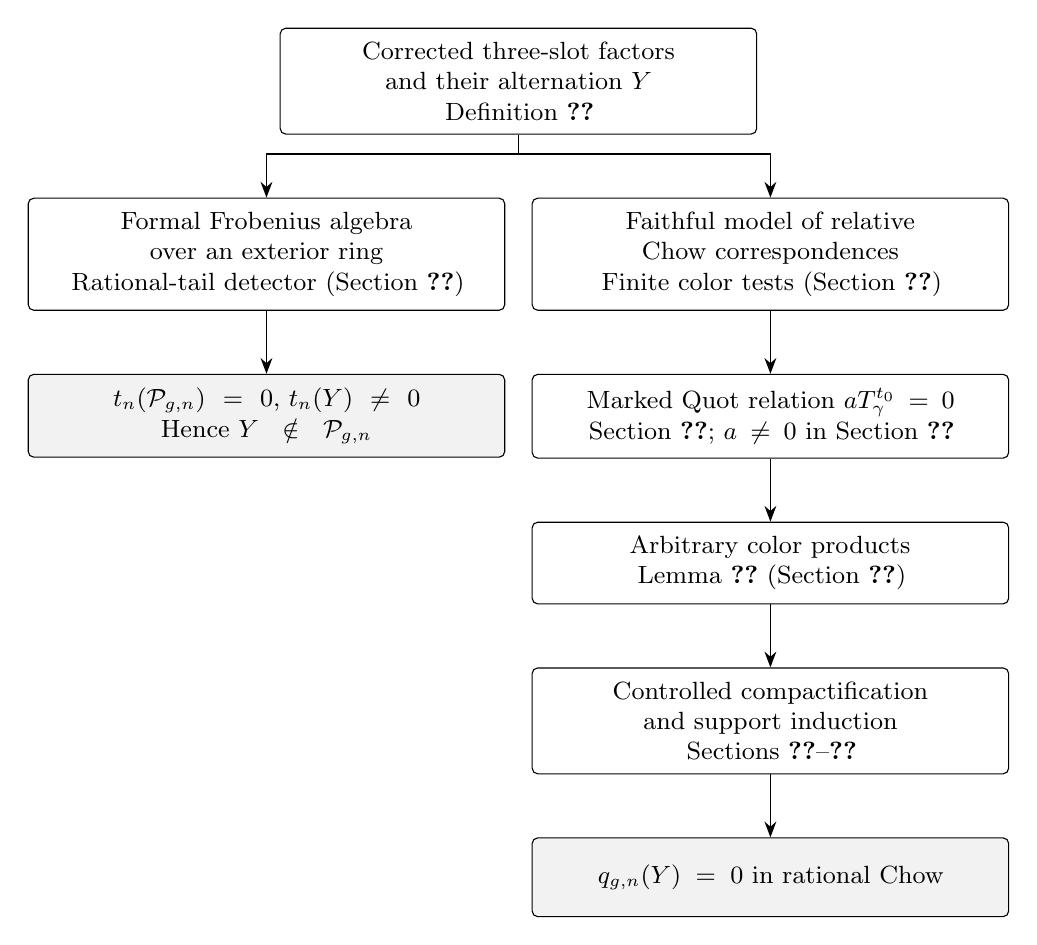
\begin{tikzpicture}[
 box/.style={draw,rounded corners=2pt,align=center,text width=5.7cm,
             minimum height=1.0cm,inner sep=5pt,font=\small},
 result/.style={box,fill=black!5},
 flow/.style={-{Stealth[length=2mm]},semithick},
 node distance=6mm]
\node[box] (candidate) {Corrected three-slot factors\\ and their alternation \(Y\)\\
 Definition~\ref{def:candidate}};
\node[box,below=8mm of candidate,xshift=-3.2cm] (formal) {Formal Frobenius algebra\\ over an exterior ring\\
 Rational-tail detector (Section~\ref{sec:detector})};
\node[box,below=8mm of candidate,xshift=3.2cm] (chow) {Faithful model of relative Chow correspondences\\
 Finite color tests (Section~\ref{sec:tensors})};
\node[result,below=8mm of formal] (outside) {\(t_n(\Pspan_{g,n})=0\), \(t_n(Y)\ne0\)\\
 Hence \(Y\notin\Pspan_{g,n}\)};
\node[box,below=8mm of chow] (surface) {Marked Quot relation \(aT_\gamma^{t_0}=0\)\\
 Section~\ref{sec:quot}; \(a\ne0\) in Section~\ref{sec:coefficient}};
\node[box,below=8mm of surface] (colors) {Arbitrary color products\\
 Lemma~\ref{lem:large-vertex-test} (Section~\ref{sec:coefficient})};
\node[box,below=8mm of colors] (boundary) {Controlled compactification\\ and support induction\\
 Sections~\ref{sec:compactification}--\ref{sec:support}};
\node[result,below=8mm of boundary] (zero) {\(q_{g,n}(Y)=0\) in rational Chow};
\draw[flow] (candidate.south) -- ++(0,-.25) -| (formal.north);
\draw[flow] (candidate.south) -- ++(0,-.25) -| (chow.north);
\draw[flow] (formal) -- (outside);
\draw[flow] (chow) -- (surface);
\draw[flow] (surface) -- (colors);
\draw[flow] (colors) -- (boundary);
\draw[flow] (boundary) -- (zero);
\end{tikzpicture}
\caption{The two assertions about the same class \(Y\). The formal
branch is independent of Chow vanishing. In the geometric branch,
the nonzero scalar completes the isotropic surface bound. The
exterior-ideal argument then gives arbitrary-color vanishing modulo base
support before the passage to the compactification.}
\label{fig:proof-map}
\end{figure}


\subsection{Conventions}

All varieties, stacks, and families are over \(\C\), and Chow groups
have rational coefficients. On a smooth space we identify Chow classes
with operational classes when pulling them to a test space.
Products of stacks are understood in rational Chow theory
\cite[Theorem~2.1.12]{Kresch}.
We use proper rational pushforward for relative Deligne--Mumford maps
and its compatibilities from \cite[Theorem~B.17 and
Propositions~B.18--B.19]{BaeSchmitt}. Smooth Deligne--Mumford stacks have
the operational identification in \cite[Theorem~C.6 and
Corollary~C.9]{BaeSchmitt}; for smooth quotient stacks, see also
\cite[Propositions~4 and~19]{EdidinGraham}.
Every formal series calculation is
truncated at a specified coefficient, so only finitely many terms occur.

Parity is distinct from Chow codimension. In a super tensor product,
interchanging homogeneous factors of parities \(p,q\) gives
\((-1)^{pq}\). In particular, on an odd vector space the
super-symmetric tensors are ordinary alternating tensors.
All finite averaging and polarization arguments take place in
characteristic zero.


\begin{table}[tb]
\centering
\small
\begin{tabular}{@{}p{.20\textwidth}p{.53\textwidth}p{.19\textwidth}@{}}
\toprule
Notation & Meaning & Definition\\
\midrule
\(\Salg_{g,n},q_{g,n},\Pspan_{g,n}\) & Formal strata algebra, Chow realization, original Pixton span & Section~\ref{sec:strata}\\
\(D_*,n,Y\) & Number of cubic factors, number of labels, candidate relation & Definition~\ref{def:candidate}\\
\(R,V,t_m\) & Exterior coefficient ring, formal Frobenius algebra, detector & Section~\ref{sec:detector}\\
\(e'_C,\eta,H_C\) & Corrected degree-one class, pure projector, complementary curve object & Section~\ref{sec:tensors}\\
\(\mathfrak B,W_b,\varphi\) & Faithful Chow coefficients, odd symplectic space, projected cubic & Proposition~\ref{prop:tensor-test}\\
\(t_0,T_\gamma,a_{N,t_0}\) & Nilpotence exponent, isotropic cubic contraction, localization scalar & Sections~\ref{sec:quot}--\ref{sec:coefficient}\\
\(F^0_{h,B},G_{h,B}\) & Corrected weighted cubic and its chosen pure lift & Section~\ref{sec:compactification}\\
\(X^\Gamma,\mathcal B_\Gamma,\mathcal S_\Gamma\) & Cut chart, compact heavy base, smooth-core open & Section~\ref{sec:compactification}\\
\bottomrule
\end{tabular}
\caption{Notation used across the proof. The formal coefficient ring
\(R\) and the faithful Chow coefficient algebra \(\mathfrak B\) have
different roles.}
\label{tab:notation}
\end{table}

\section{The strata algebra and the explicit class}\label{sec:strata}

This section fixes the relation space. The distinction between an
unnormalized gluing generator and an automorphism-weighted graph sum
will be used in both parts of the proof.

\subsection{Decorated graphs}

A stable graph \(\Gamma\) of type \((g,n)\) is a connected graph with
\(n\) labeled legs and genera \(g_v\geq0\) at its vertices, satisfying
\[
g=\sum_{v}g_v+|E(\Gamma)|-|V(\Gamma)|+1,
\qquad 2g_v-2+n_v>0.
\]
Here \(n_v\) counts all incident half-edges, including legs. Its gluing
map is
\[
\xi_\Gamma\colon\prod_{v\in V(\Gamma)}
\Mbar_{g_v,n_v}\longrightarrow\Mbar_{g,n}.
\]
At every half-edge let \(\psi\) denote the cotangent class. At a vertex
define
\[
\kappa_j=\pi_*(\psi_{n_v+1}^{j+1}),\qquad
\kappa_0=2g_v-2+n_v,
\]
where \(\pi\) forgets an additional marking.

The vector space \(\Salg_{g,n}\) is spanned by formal symbols
\([\Gamma,\gamma]\), modulo graph isomorphism, with \(\gamma\) a monomial
in the half-edge \(\psi\)'s and vertex \(\kappa_j\)'s for \(j\geq1\).
At each vertex its decoration degree is at most \(3g_v-3+n_v\).
The total degree is \(|E(\Gamma)|+\deg\gamma\), and
\[
q_{g,n}[\Gamma,\gamma]=\xi_{\Gamma*}(\gamma).
\]
There is no automorphism denominator in this definition of \(q_{g,n}\).
The per-vertex degree bound is the explicit convention in
\cite[Section~0.3]{PPZ}.

We use the usual decorated-graph intersection product. More explicitly,
take common refinements with specified contractions to fixed
representatives of the input graphs, requiring every refined edge to
survive in at least one contraction. Divide by the source symmetries
preserving those contractions. For each additional use of an overlapping
edge insert its normal factor \(-\psi-\psi'\); pull the leg and flag
decorations to their components and split kappa classes additively.
Specified contractions record the lifts to the gluing parameter spaces,
so this convention gives the product of the \emph{unnormalized}
pushforward generators. The construction is the transverse and
self-intersection rule for node cuts
\cite[Appendix~A, Proposition~9 and Equation~(11)]{GraberPandharipande2003}.

Terms exceeding any vertex dimension are set to zero. For multiplication
and restriction to a further graph splitting, an excessive decoration
remains excessive: the combined dimensions on the pieces decrease,
so at least one piece still exceeds its dimension.
Forgetting pullback of an undecorated graph is obtained by adding
the new leg successively at each vertex. These conventions lift the
corresponding Chow operations and do not impose any unproved relation.
The preceding dimension argument is not an assertion about forgetting,
which raises a vertex dimension. Compatibility of forgetting with the
formal detector is checked separately in Section~\ref{sec:detector}.

\subsection{The exact Pixton span}

Define
\[
A(T)=\sum_{m\geq0}\frac{(6m)!}{(3m)!(2m)!}T^m,\qquad
B(T)=\sum_{m\geq0}
\frac{6m+1}{6m-1}\frac{(6m)!}{(3m)!(2m)!}T^m.
\]
For a commuting parity variable \(\zeta^2=1\), put
\[
\widehat C_{3j}(T,\zeta)=T^jA(\zeta T),\qquad
\widehat C_{3j+1}(T,\zeta)=\zeta T^jB(\zeta T).
\]
Indices congruent to \(2\) modulo \(3\) are not used. For a series \(F\)
write
\[
\{F\}=\sum_{m\geq0,\ \epsilon\in\{0,1\}}
[F]_{T^m\zeta^\epsilon}K_{m,\epsilon}T^m.
\]
Give every vertex of \(\Gamma\) its own variable \(\zeta_v\), with
\(\zeta_v^2=1\). Define the operator
\[
\widehat\kappa_\Gamma
\left(\prod_{i=1}^{\ell}K_{e_i,\epsilon_i}\right)
=
\sum_{\tau\in\mathfrak S_\ell}
\prod_{\substack{c\text{ a cycle}\\\text{of }\tau}}
\left(
\sum_{v\in V(\Gamma)}
\kappa^{(v)}_{\sum_{i\in c}e_i}
\zeta_v^{\sum_{i\in c}\epsilon_i}
\right).
\]
The empty product maps to \(1\), and the operator acts coefficientwise
in \(T\). The permutation-cycle expression is Faber's formula, as
recorded in \cite[Equations~(1.12)--(1.13)]{ArbarelloCornalba1996}.

For an edge whose two half-edges lie at \(v,w\), with cotangent symbols
\(x,y\), set
\[
\Delta_e=
\frac{
A(\zeta_vxT)\zeta_wB(\zeta_wyT)
+\zeta_vB(\zeta_vxT)A(\zeta_wyT)
+\zeta_v+\zeta_w
}{(x+y)T}.
\]
This is a power series by
\[
A(T)B(-T)+A(-T)B(T)+2=0.
\]
The same rule applies to a loop.

\begin{definition}[Pixton's original span]\label{def:pixton-span}
Let \(\sigma=(\sigma_1,\ldots,\sigma_\ell)\) be a partition with no
part congruent to \(2\) modulo \(3\), possibly empty, and let
\(a_1,\ldots,a_n\geq0\) also avoid that residue class.
For \(0\leq r\leq3g-3+n\), require
\begin{equation}\label{eq:pixton-admissibility}
3r\geq g+1+|\sigma|+\sum_i a_i,\qquad
3r\equiv g+1+|\sigma|+\sum_i a_i\pmod2.
\end{equation}
Set
\begin{align}
P_\Gamma={}&
\left[
2^{-h^1(\Gamma)}
\widehat\kappa_\Gamma
\left(
\exp\{1-\widehat C_0\}
\prod_{j=1}^{\ell}\{\widehat C_{\sigma_j}\}
\right)\right.\notag\\
&\left.\hspace{12mm}\cdot
\prod_{i=1}^n\widehat C_{a_i}(\psi_iT,\zeta_{v(i)})
\prod_{e\in E(\Gamma)}\Delta_e
\right]_{T^{r-|E(\Gamma)|}\prod_v\zeta_v^{g_v+1}},
\label{eq:pixton-graph}
\end{align}
where \(h^1(\Gamma)=|E|-|V|+1\), \(v(i)\) carries the \(i\)-th leg,
and parity exponents are read modulo \(2\). In braces, the arguments
of \(\widehat C_i\) are \(T,\zeta\). A negative requested \(T\)-degree
means zero. The relation is
\[
\mathcal R(g,n,r;\sigma,a)=
\sum_\Gamma\frac{[\Gamma,P_\Gamma]}{|\Aut\Gamma|}.
\]

The space \(\Pspan_{g,n}\subseteq\Salg_{g,n}\) is the following
linear span in each degree. Choose an outer stable graph of type
\((g,n)\); put one such relation at one vertex, and arbitrary decorated
strata elements at all other vertices; then glue, using the
unnormalized gluing operation. Take the span over every choice,
including the graph with one vertex and no edges.
\end{definition}

\begin{proposition}[Known validity and stability]\label{prop:known-relations}
The span in Definition~\ref{def:pixton-span} is an ideal and is stable
under tautological gluing and forgetting pushforwards and pullbacks.
For gluing pullback to a product, the target relation space is the sum
of the spaces with a relation in one factor.
Moreover
\[
\Pspan_{g,n}\subseteq\ker q_{g,n}.
\]
\end{proposition}

\begin{proof}
The ideal and operation statements are
\cite[Proposition~1]{Pixton} for precisely this original span.
Chow validity of the \(a_i\in\{0,1\}\) seed relations follows from
\cite[Theorem~1 and its reconstruction]{Janda}.
The construction in \cite[Section~3.5]{PPZ} generates the higher
marking indices by psi multiplication, the partition insertions by
forgetting extra markings, and the outer-graph relations by gluing.
These are formal identities, so they apply to the Chow-valid seeds.
The parity condition in \eqref{eq:pixton-admissibility} converts the
strict seed inequality to the displayed admissibility inequality.
In Janda's reconstructed normalization, a degree-\(r\) seed is
\((-1)^{\sum_i a_i}(-1/1728)^r\) times the empty-partition recipe
above. This nonzero scalar does not change its vanishing or its span.
\end{proof}

No converse to Proposition~\ref{prop:known-relations} is used.
In particular, same-vertex multiplication of a relation does not enlarge
the span, whereas an arbitrary new Chow relation is not assumed to
belong to it.

\subsection{The corrected cubic and its alternation}

For the rest of the construction fix
\begin{equation}\label{eq:global-parameters}
g=10^{60},\qquad D_*=\binom g3,\qquad n=3D_*.
\end{equation}
Form a word \(\mathbf i\) in the colors \(1,\ldots,g\) by concatenating
all increasing triples of colors in lexicographic order. Its consecutive
three-slot blocks will be denoted \(J\). Each color occurs
\(\binom{g-1}{2}\) times.

For a set of labels \(T\) of size at least two, let \(D_T\) be the
one-edge class cutting off a genus-zero tail with precisely those
labels. For distinct labels \(a,b\), put
\[
\bar D_{ab}=\sum_{T\supseteq\{a,b\}}D_T.
\]
We also need a class supported on rational bridges, not tails.

\begin{definition}[The explicit counterexample]\label{def:candidate}
On three labeled slots \(J=(a,b,c)\), take every one-edge
\emph{unmarked} stable graph of genus \(g\), subdivide its edge by
a genus-zero vertex, and put all three labels at that new vertex.
Sum the resulting undecorated graphs, dividing each by its automorphism
order. Pull this sum back by forgetting all labels outside \(J\);
call the resulting class \(\beta_J^{\mathrm{st}}\).

Define
\begin{equation}\label{eq:candidate}
F_J^{\mathrm{st}}=
\bar D_{ab}\bar D_{ac}-\frac12\beta_J^{\mathrm{st}},
\qquad
Y=\sum_{\substack{\tau\in\mathfrak S_n\\\tau\mathbf i=\mathbf i}}
\operatorname{sgn}(\tau)\,
\tau\left(\prod_J F_J^{\mathrm{st}}\right).
\end{equation}
Here \(\tau\) relabels slots, and products and forgetting pullbacks
are the formal graph operations fixed above.
\end{definition}

Every operation in Definition~\ref{def:candidate} is finite.
Each cubic factor has codimension two, so
\[
\deg Y=2D_*<3g-3+n.
\]
The pair \((g,n)\) is stable. The automorphism weights in
\(\beta_J^{\mathrm{st}}\) specify coefficients of this particular
class; they do not change the unnormalized generators of
\(\Salg_{g,n}\).

The proof of Theorem~\ref{thm:main} now divides into two independent
claims. Proposition~\ref{prop:detector} proves formal nonmembership.
The remaining sections establish the geometric vanishing
in Theorem~\ref{thm:chow-vanishing}.

\section{A formal detector}
\label{sec:detector}

We first separate the candidate from the relation space.  Throughout this
section the genus \(g\) is fixed as in Definition~\ref{def:candidate},
but the number of labels is allowed to vary, including zero.
No Chow relation on a positive-genus vertex will be imposed in the
construction.

\begin{proposition}
\label{prop:detector}
There are a supercommutative \(\Q\)-algebra \(R\), a finite free
supermodule \(V\) over \(R\), and \(\Q\)-linear maps
\[
 t_m:\Salg_{g,m}\longrightarrow V^{\otimes_R m}
 \qquad(m\geq 0)
\]
such that \(t_m(\Pspan_{g,m})=0\) for every \(m\), whereas
\(t_n(Y)\neq0\).  In particular \(Y\notin\Pspan_{g,n}\).
\end{proposition}

The maps are tests on formal strata.  In particular, they are not
asserted to factor through the Chow ring.

\subsection{An isotropic cubic Frobenius algebra}

The state space has the curve pairing familiar from Frobenius-algebra
and CohFT constructions \cite{Abrams1996,PZ2019}. The exterior
coefficient ring below allows an independent cubic on every triple of
colors. We check associativity and the handle formula directly, since
these particular identities govern the graph test.

Let
\[
 R=\Lambda_{\Q}\bigl(\theta_{ijk}:1\leq i<j<k\leq g\bigr),
\]
with each generator odd.  Let \(W\) be a purely odd symplectic vector
space of dimension \(2g\), with complementary Lagrangians
\(W_+\) and \(W_-\).  Choose bases \(a_1,\ldots,a_g\) and
\(b_1,\ldots,b_g\) such that
\(\langle a_i,b_j\rangle=\delta_{ij}\).
Extend the symbols \(\theta_{ijk}\) alternately to all triples of
indices.  There is an alternating, odd-coefficient three-form
\(\Phi\) on \(W\) defined by
\[
 \Phi(a_i,a_j,a_k)=\theta_{ijk},
 \qquad
 \Phi(w_1,w_2,w_3)=0
 \quad\text{if some }w_i\in W_-.
\]

Consider the free supermodule
\[
 V=R\otimes_{\Q}\bigl(\Q1\oplus W\oplus\Q e\bigr),
\]
where \(1,e\) are even.  Its trace, denoted by \(\int\), takes \(e\)
to \(1\) and is zero on \(1,W\).  Give \(V\) the even pairing which
is hyperbolic on \(\Q1\oplus\Q e\), the prescribed symplectic pairing
on \(W\), and zero between these two summands.  Declare \(1\) to be
the unit, \(e^2=eW=0\), and determine the remaining products by
\[
 \int w_1w_2=\langle w_1,w_2\rangle,
 \qquad
 \int w_1w_2w_3=\Phi(w_1,w_2,w_3).
\]
Equivalently, the product of two standard odd vectors is its
symplectic pairing times \(e\), plus the vector dual to the cubic
functional in the third input.  The latter vector has odd
coefficients and belongs to \(R\otimes W_-\).

Write \(\mu\) for multiplication and \(\Delta\) for its adjoint
coproduct.

\begin{lemma}
\label{lem:detector-algebra}
These rules give a supercommutative associative Frobenius algebra.
The product of three standard odd vectors belongs to \(Re\), and
the product of four such vectors is zero.  Its handle element is
\[
 \mu\Delta(1)=(2-2g)e.
\]
\end{lemma}

\begin{proof}
The pairing is nondegenerate, so the rules determine the product.
Supercommutativity follows from alternation of the symplectic form
and of \(\Phi\), with coefficients moved using the super sign rule.
For example,
\[
 a_i a_j=-\sum_k\theta_{ijk}b_k,
 \qquad a_i b_j=\delta_{ij}e,
\]
and therefore \((a_i a_j)a_k=\theta_{ijk}e
=a_i(a_j a_k)\).

More generally, pair the associator of three vectors from \(W\)
with a fourth basis vector.  Pairing with \(1\) gives the cyclic
symmetry of the alternating cubic, and pairing with \(e\) gives
zero.  If the fourth vector is in \(W\), both expressions are
contractions of two pair-product tensors.  Their \(W\)-channel
contractions vanish because the cubic is supported on a
Lagrangian; their hyperbolic-channel contractions vanish because
\(e^2=eW=0\).  Nondegeneracy proves associativity.  Cases involving
\(1\) or \(e\) are immediate.  The same product description proves
the assertions about three and four odd inputs.

The hyperbolic channels contribute \(2e\) to the handle element,
and the \(2g\) odd channels contribute \(-2ge\).  The cubic
perturbation has zero internal trace, because a symplectic
contraction pairs the two different Lagrangians.  This gives the
displayed formula.
\end{proof}

Set
\[
 \lambda=(2g-2)e.
\]
For a nonempty finite label set \(L\), write
\(\Delta_L:V\to V^{\otimes L}\) for the coproduct adjoint to
iterated multiplication; for a singleton it is the identity.
Coproducts are coassociative and satisfy the projection formula.
In particular, writing \(\Delta_{ij}(1)\) with units in all other
slots, we have
\begin{align}
 \Delta_{ij}(1)\Delta_{ik}(1)&=\Delta_{ijk}(1), \label{eq:detector-diagonals}\\
 \Delta_{ij}(1)^2&=-\Delta_{ij}(\lambda). \label{eq:detector-self}\\
 \int_j\Delta_{ij}(v)&=v. \label{eq:detector-counit}
\end{align}
The minus sign in \eqref{eq:detector-self} will match the normal
bundle of a rational-tail boundary divisor.

\subsection{Compression of rational tails}

Call a graph a \emph{rational-tails graph} if it is a tree with one
genus-\(g\) vertex, called its root, and all other vertices rational.
Every branch away from the root has nonempty labeled descendants.
Such a graph has no automorphisms fixing the labels: the descendant
label sets distinguish its branches, recursively.

We initially work without the degree cutoff, discard all graphs
which are not rational-tails graphs, and allow genuine genus-zero
Chow identities on rational parameter factors.  This is only an
auxiliary computation; we will prove that its output respects the
cutoff in \(\Salg_{g,m}\). We use the genus-zero Chow boundary
presentation of \cite[Section~4, Theorem~1]{Keel1992}.

For each label \(i\), put
\[
 \bar\psi_i=\psi_i-\sum_{\substack{T\ni i\\ |T|\geq2}}D_T.
\]
If the labels are ordered \(1,\ldots,m\), let \(L_x\) be the
pullback of \(\psi_x\) from the space retaining just
\(1,\ldots,x\).  Thus
\[
 L_x=\psi_x-
 \sum_{\substack{T\ni x,\ |T|\geq2\\T\setminus\{x\}\subseteq\{x+1,\ldots,m\}}}
 D_T.
\]
For \(j\geq1\), define
\[
 \bar\kappa_j=\kappa_j-\sum_{x=1}^m L_x^j.
\]
The leading, graphless change of variables is
\(\bar\psi_i=\psi_i\) and
\(\bar\kappa_j=\kappa_j-\sum_i\psi_i^j\), which is an invertible
polynomial change.  Hence the bar monomials form a complement to
the boundary subspace before truncation.

Define \(t_m\) on that complement by
\begin{equation}
 t_m\left(\prod_i\bar\psi_i^{d_i}
                 \prod_{j\geq1}\bar\kappa_j^{c_j}\right)
 =
 \begin{cases}
   \lambda_1^{d_1}\cdots\lambda_m^{d_m},
      &\text{if every }c_j=0,\\
   0,&\text{otherwise}.
 \end{cases}
 \label{eq:detector-prescription}
\end{equation}
Here the tensor on the right has a unit in every unused slot.
For a nontrivial rational-tails graph, integrate each non-root
decoration on its genus-zero parameter space, retaining only its
top-degree integral.  Apply \(t_a\) to the decorated root with its
\(a\) incident slots.  Finally duplicate each root slot into the
descendant labels of its branch by \(\Delta_L\).
Every branch attached to the root has at least two descendant
labels, so \(a<m\); this is a recursive definition.  For \(m=0\),
the empty tensor is \(R\), the unit maps to \(1\), and positive
bar-kappa monomials map to zero.

\begin{lemma}
\label{lem:detector-cutoff}
The prescription is well defined modulo genuine relations on
rational parameter factors and induces a map on \(\Salg_{g,m}\).
For a homogeneous expression of degree \(r\), its image is a sum
of tensors indexed by partitions of the labels into nonempty
blocks, of the form
\begin{equation}
 \bigotimes_{L}\Delta_L(\lambda^{d_L}),
 \qquad
 r=\sum_L\bigl(|L|-1+d_L\bigr).
 \label{eq:detector-blocks}
\end{equation}
In particular \(t_m\) is zero in degrees \(r>m\).
\end{lemma}

\begin{proof}
Grafting a genus-zero graph amounts to composing coproducts and
multiplying the corresponding integrals.  Coassociativity shows
that the result is independent of the internal decomposition of
a rational parameter class.  In particular a zero class on such
a factor contributes zero.

For a rational subtree with \(k\) descendant labels, top
decoration degrees together with its edges, including the edge
attaching it to the root, add to \(k-1\).  Formula \eqref{eq:detector-blocks} follows by
induction, starting from the bar prescription.  Since
\(\lambda^2=0\), a nonzero term has \(d_L\leq1\), and hence \(r\leq m\).

An excessive decoration on a rational vertex has zero integral.
At a root with \(a\) incident slots, a decoration exceeding
\(3g-3+a\) also exceeds \(a\), and its recursive test is zero.
This applies since \(g\geq2\).  Finally, under refinement the sum
of the dimensions of the pieces of a vertex decreases by the
number of new edges.  Splitting a decoration additively between
those pieces cannot make an excessive total degree admissible
on every piece.  Thus discarded terms also remain invisible
under multiplication and refinement.  Forgetting operations
require a separate argument, supplied below.
\end{proof}

\subsection{Boundary operations and the test}

We first show how the test treats multiplication by bar classes and
rational-tail divisors.  We then prove the forgetting identities
that will reduce the number of labels in the relation argument.
All tensor products, contractions, and permutations below use
the super sign convention.

\begin{lemma}[Boundary operations]
\label{lem:detector-operations}
The maps \(t_m\) are equivariant for relabeling.  For every
strata expression \(b\), they satisfy
\begin{align}
 t(\bar\psi_i b)&=\lambda_i t(b),
 &t(\bar\kappa_j b)&=0, \label{eq:detector-bars}\\
 t(\bar D_{ij}b)&=\Delta_{ij}(1)t(b). \label{eq:detector-pair}
\end{align}
More generally, gluing along \(D_T\) integrates the entire
genus-zero input and duplicates the root-side attaching slot
into the labels of \(T\).
\end{lemma}

\begin{proof}
We first establish the boundary restrictions and the graph
compatibilities used in the calculation. The descendant and kappa
identities are the forgetting and gluing formulas in
\cite[Equations~(1.7)--(1.10)]{ArbarelloCornalba1996}.  At the gluing for
\(D_T\), let \(p\) be the root-side flag and \(p'\) the
rational-side flag.  The normal class is
\(-\psi_p-\psi_{p'}\).  On
\(\Mbar_{0,T\cup\{p'\}}\), the sum of boundary splits separating
\(i\) from \(p'\) equals \(\psi_i+\psi_{p'}\).  The sum whose
side away from \(p'\) contains two fixed labels \(i,j\) equals
\(\psi_{p'}\).  These are the genus-zero cotangent boundary
formulas; they also follow by successively forgetting to three
labels and applying the cotangent pullback formula.

Consequently, \(\bar\psi_i\) restricts to the modified cotangent
of its ancestor slot on the root side, using \(p\) if \(i\in T\).
The restriction of \(\bar D_{ij}\) is the analogous pair class
on the root side, except when both labels lie in \(T\), when it
is \(-\bar\psi_p\).

The class \(\bar\kappa_j\) is independent of the chosen ordering.
Indeed, for two consecutive labels made last, write
\(D=D_{\{i,j\}}\).  The identities
\(\psi_i|_D=\psi_j|_D=0\) and
\(D|_D=-\psi_p\) give, for \(d\geq1\),
\begin{equation}
  (\psi_i-D)^d-\psi_i^d=-D\psi_p^{d-1}
  =(\psi_j-D)^d-\psi_j^d.
 \label{eq:detector-order}
\end{equation}
After pulling to the remaining labels, this is precisely the
invariance under a consecutive transposition.  To restrict
\(\bar\kappa_j\) to \(D_T\), put the labels of \(T\) last.
The kappa class splits additively between the two vertices.
The first label of \(T\) gives the root-side cotangent at \(p\);
the remaining partial cotangents on the rational factor cancel
its kappa class by the forgetful kappa formula.  The result is
exactly \(\bar\kappa_j\) on the root side.

These restrictions and the coproduct projection formula prove
\eqref{eq:detector-bars} recursively, beginning with \eqref{eq:detector-prescription}.
For \eqref{eq:detector-pair}, only the two-label tail has a
nonzero undecorated integral.  If \(i,j\) are in different
branches, the root-side pair class joins their ancestor slots.
If they are in the same branch, its restriction is
\(-\bar\psi_p\), and the required identity is
\eqref{eq:detector-self}.  This proves the assertion for an
arbitrary boundary expression as well as for a bar monomial.
The gluing assertion follows directly by coassociativity and
the factorization of genus-zero integrals.

These calculations take place in the auxiliary formal graph space
modulo relations on rational parameter factors.  Simultaneous
compatible splits produce the same tree independently of their
order, with one normal factor for every repeated edge.  Hence the
polynomial multiplications used here commute and associate.
A genuine zero on a rational factor remains zero: restriction
there is a genuine genus-zero operation, and operations at another
factor retain that zero with relabeled flags.
Lemma~\ref{lem:detector-cutoff} permits the dimension truncations.
Graphs outside the rational-tails locus remain outside it under
refinement, so their products contribute zero as well.

Finally, independence of the bar-kappa ordering, the restriction
formulas, and the symmetric coproduct construction give
equivariance under arbitrary relabeling.
\end{proof}

\subsection{Forgetting markings}

The forgetting identities are needed in both directions: pullback
will remove a zero-index leg from the Pixton recipe, and pushforward
will test a tensor slot against the two even basis vectors.

\begin{lemma}[Forgetting operations]
\label{lem:detector-forgetting}
For every strata expression \(b\), the maps \(t_m\) satisfy
\begin{equation}
 t(\pi_y^*b)=t(b)\otimes1,
 \qquad
 t(\pi_{y*}b)=\int_y t(b).
 \label{eq:detector-forget}
\end{equation}
Here \(\pi_y\) forgets the label \(y\); the identities hold
in any order of the remaining labels.
\end{lemma}

\begin{proof}
We first calculate before the degree cutoff, modulo genuine
genus-zero relations, and check at the end that every discarded
term has zero test after forgetting.  No relation on a
positive-genus parameter factor enters the calculation.

\paragraph{Formal pullback and projection.}
Forget pullback adds
\(y\) at every possible vertex.  At that vertex it replaces
\begin{equation}
 \psi_h\longmapsto\psi_h-D_{\{h,y\}},
 \qquad
 \kappa_j\longmapsto\kappa_j-\psi_y^j.
 \label{eq:detector-vertex-pull}
\end{equation}
A tail divisor pulls back as \(D_T+D_{T\cup\{y\}}\).
Against a tree, an incompatible split remains incompatible;
a compatible new edge splits a vertex.  If the split edge
already occurs, the two pullback terms give its pulled normal
class: adding \(y\) at an endpoint adds the boundary term
cutting off that half-edge together with \(y\).  Thus pullback
commutes with multiplication by the indicated polynomial
classes.

The push-projection calculation is equally local.  At a stable
vertex, put
\[
 X_i=\pi_y^*\psi_i,\qquad k_j=\pi_y^*\kappa_j,\qquad
 d_i=D_{\{i,y\}},
\]
so that \(\psi_i=X_i+d_i\) and
\(\kappa_j=k_j+\psi_y^j\).  The relevant rules are
\begin{equation}
 d_i d_l=0\ (i\neq l),\qquad
 d_i^2=-X_i d_i,\qquad
 \psi_y d_i=0,
 \label{eq:detector-forget-products}
\end{equation}
and
\begin{equation}
 \pi_{y*}1=0,\qquad
 \pi_{y*}\psi_y^d=\kappa_{d-1}\ (d\geq1),\qquad
 \pi_{y*}d_i=1.
 \label{eq:detector-forget-push}
\end{equation}
They prove projection with graphless cotangent and kappa
polynomials by substitution.  For a tail multiplier, its two
pullback splits distribute the \(\kappa_{d-1}\) in \eqref{eq:detector-forget-push}
additively over the two vertices; for \(d_i\), exactly the
compatible split pushes to the original tail.  On a tree with
a stable \(y\)-vertex this reduces to the same vertex
calculation.  If forgetting contracts a three-point vertex
with a surviving terminal label, the compatible split places
\(y\) with that label.  If it contracts a bridge, the two
normal contributions add to the normal of the combined edge.
All other compatible splits lift uniquely.  This proves the
needed push projection on boundary graphs as well.

Forgetting also preserves the rational-factor relations used in
the auxiliary computation: its pullbacks and pushforwards on
those factors are actual genus-zero operations.  Operations at
another factor retain a rational-factor zero with relabeled flags.

\paragraph{Pullback of the test.}
Both bar classes
pull to themselves.  On a boundary graph, adding \(y\) to a
rational factor increases its dimension without increasing
the pulled decoration degree, so its integral is zero.
Adding \(y\) at the root uses the smaller recursive pull
identity.  This proves the pull assertion.

\paragraph{Pushforward of the test.}
For pushforward on a boundary graph, forgetting on a rational
factor commutes with its integral; a three-point contraction
uses the counit identity \eqref{eq:detector-counit}.
Forgetting at the root again uses the smaller recursive
assertion.  On the bar-monomial complement, projection reduces
the question to powers of \(\bar\psi_y\), since all other bar
classes are pulled back.  The zeroth power pushes to zero.
For \(d>0\), telescope
\begin{equation}
 \psi_y^d-\bar\psi_y^d
 =
 \sum_{\varnothing\neq S}
 D_{S\cup\{y\}}\sum_{a=0}^{d-1}
        \psi_y^{d-1-a}\bar\psi_y^a.
 \label{eq:detector-telescope}
\end{equation}
On the rational tail with labels \(S\cup\{y\}\), the dimension
is \(|S|-1\), and only the term \(a=d-|S|\) integrates.
Its integral is
\(\int_{\Mbar_{0,|S|+2}}\psi_y^{|S|-1}=1\).
After pushforward and application of the test, \eqref{eq:detector-telescope} is
therefore
\begin{equation}
 \sum_{1\leq |S|\leq d}\Delta_S(\lambda^{d-|S|}),
 \label{eq:detector-tail-sum}
\end{equation}
with units in all unused slots.

On the other hand,
\begin{equation}
 t_m(\kappa_{d-1})
 =
 \int\lambda^d+
 \sum_{1\leq |S|\leq d}\Delta_S(\lambda^{d-|S|}).
 \label{eq:detector-kappa}
\end{equation}
For \(d=1\) this is the scalar identity
\(\kappa_0=2g-2+m\).
For \(d>1\), expand
\(\kappa_{d-1}=\bar\kappa_{d-1}+\sum_xL_x^{d-1}\).
Before pulling from the stage with labels \(1,\ldots,x\),
write the exact polynomial identity
\begin{equation}
 \psi_x^{d-1}-\bar\psi_x^{d-1}
 =
 \sum_{\substack{T\subseteq\{1,\ldots,x\}\\x\in T,\ |T|\geq2}}
 D_T\sum_{a=0}^{d-2}
       \psi_x^{d-2-a}\bar\psi_x^a .
 \label{eq:detector-partial-telescope}
\end{equation}
On the tail for \(T\), the dimension is \(|T|-2\).
Thus its integral selects exactly \(a=d-|T|\), when that
exponent lies between \(0\) and \(d-2\), and the integral
of \(\psi_x^{|T|-2}\) is \(1\).  The remaining bar cotangent
is the root-side cotangent, so this term contributes
\(\Delta_T(\lambda^{d-|T|})\), with coefficient \(+1\).
The term \(\bar\psi_x^{d-1}\) gives the singleton \(T=\{x\}\).
Pulling through the later labels adds only unit tensor
slots, by the pull identity already proved.  Every block
therefore occurs once, indexed by its largest label, with
no binomial coefficient or normal self-intersection sign.
Subtracting \eqref{eq:detector-tail-sum}
from \eqref{eq:detector-kappa} proves
\(t_m(\pi_{y*}\bar\psi_y^d)=\int\lambda^d\), as required.

\paragraph{Compatibility with the cutoff.}
A non-rational-tails graph stays outside the test under forgetting:
its nontrivial unmarked stabilization persists.

We must also check forgetting on terms discarded by the
vertexwise cutoff; this does not follow from the refinement
dimension argument alone.  An excessive decoration on a
rational factor is an actual zero in its genus-zero Chow
ring.  Its genuine forget pullback or pushforward is still
zero, including the integral used when a three-point factor
contracts.  Operations on another factor preserve this
rational-factor zero.
For an excessive root decoration of degree \(d\) with
\(a\) root slots, we have \(d\geq3g-2+a\).  Adding a mark
at that root gives an expression of degree \(d>a+1\),
so the block bound kills its test with \(a+1\) slots.
Forgetting a root mark gives degree \(d-1>a-1\), killed
by the same bound with \(a-1\) slots.  The root stays stable
because \(g\geq2\).  Adding or forgetting on a rational
factor leaves the root decoration unchanged; a contracted
rational three-point vertex merely replaces an attaching
flag without changing the root arity.
Thus discarded terms have zero test before and after each
forget operation.  Together with
Lemma~\ref{lem:detector-cutoff}, this permits every cutoff
in the displayed test identities.  It does not assert that
untruncated pullback descends unchanged to the truncated
formal algebra.
Equivariance from Lemma~\ref{lem:detector-operations} allows
the forgotten label to be placed last in any chosen order.
\end{proof}

\subsection{The zero-leg identity}

We require one precise identity for the recipe in
Definition~\ref{def:pixton-span}.  Package the partition
insertions with formal variables \(s_\ell\), one for each
allowed positive part, using exponential coefficients for
repeated parts, and put
\[
 H(T,\zeta)=\widehat C_0(T,\zeta)
             -\sum_\ell s_\ell\widehat C_\ell(T,\zeta).
\]
The variables \(s_\ell\) are purely formal; all subsequent
coefficient extractions involve finitely many of them. The logarithm
below is expanded jointly in \(T\) and the \(s_\ell\), so its constant
term at \(T=s_\ell=0\) is defined even though \(H(0,\zeta)\) depends
on the partition variables.
The cycle exponential formula for \(\widehat\kappa_\Gamma\)
rewrites the vertex characteristic as
\begin{equation}
 \exp\{-\log H\}_{\kappa,\zeta_v}.
 \label{eq:detector-characteristic}
\end{equation}
Here a monomial \(T^d\zeta^\epsilon\) in \(-\log H\) is
replaced by \(\kappa_dT^d\zeta_v^\epsilon\), including \(d=0\).
For the edges use \(U(x,x')=T\Delta_e\), so the coefficient
of total degree \(T^r\) is the degree-\(r\) recipe.
Denote this packaged series, with its usual parity
extractions, by \(\mathcal R(s;a)\).

\begin{lemma}
\label{lem:detector-unit}
If all preceding leg indices \(a_j\) are zero or one, then,
in the untruncated rational-tails computation,
\begin{equation}
 \mathcal R(s;a,0)
 -\sum_\ell s_\ell\mathcal R(s;a,\ell)
 =\pi_y^*\mathcal R(s;a).
 \label{eq:detector-unit}
\end{equation}
\end{lemma}

\begin{proof}
The kappa pullback formula, including
\(\kappa_0^{\mathrm{old}}=\kappa_0^{\mathrm{new}}-1\),
multiplies the new characteristic \eqref{eq:detector-characteristic} by
\(H(\psi_yT,\zeta_v)\).  This is exactly the linear
combination of new leg factors on the left.

It remains to check bubbles introduced in pulling the old
leg and half-edge cotangents.  For a function \(f(x)\), this
pull gives the boundary correction
\((f(0)-f(x))/x\), where \(x\) is the stable-side cotangent.
At a new rational three-point vertex, its characteristic is
\(H(0,\epsilon)^{-1}\); the new \(H\)-leg cancels it.
Let \(\eta,\eta'\) be stable-side parity variables, and write
\[
 A_x=A(\eta xT),\quad B_x=B(\eta xT),
 \qquad
 A_{x'}=A(\eta'x'T),\quad B_{x'}=B(\eta'x'T).
 \]
The edge adjoining that bubble has factor
\begin{equation}
 \frac{\eta(B_x+1)+\epsilon(1-A_x)}{x}.
 \label{eq:detector-bubble-edge}
\end{equation}
If the bubble carries an old leg, its constant factor is
\(1\) or \(-\epsilon\).  Extracting \(\epsilon\) in \eqref{eq:detector-bubble-edge}
then gives \((1-A_x)/x\) or
\(-\eta(B_x+1)/x\), respectively.  These are exactly the
two divided differences.

If the bubble subdivides an old edge, the coefficient of
\(\epsilon\) in the product of its two edge factors is
\begin{equation}
 \frac{\eta(B_x+1)(1-A_{x'})
       +\eta'(B_{x'}+1)(1-A_x)}{xx'}.
 \label{eq:detector-bubble-product}
\end{equation}
Substituting the original edge numerator shows that \eqref{eq:detector-bubble-product}
equals
\begin{equation}
 \frac{U(0,x')-U(x,x')}{x}
 +\frac{U(x,0)-U(x,x')}{x'}.
 \label{eq:detector-edge-difference}
\end{equation}
Thus it also gives precisely the two cotangent pullback
corrections.  Bubbles for distinct slots at a vertex are
disjoint, and these are all possibilities for adding one
mark.  Finally, rational-tails graphs have \(h^1=0\) and
trivial automorphism groups, so neither the factor
\(2^{-h^1}\) nor unnormalized gluing introduces another
coefficient.  This proves the identity.
\end{proof}

\subsection{Annihilating the relation span}

\begin{lemma}
\label{lem:detector-annihilation}
For every \(m\geq0\), \(t_m(\Pspan_{g,m})=0\).
\end{lemma}

\begin{proof}
We induct first on arity.  At a fixed arity, the induction already
kills every nontrivial outer gluing and every relation multiplied
by a tail divisor.  With those terms disposed of, degree and
partition length reduce the basic recipes to the all-ones case,
where an alternating-form calculation finishes the argument.

Use the precise span and operation stability in
Proposition~\ref{prop:known-relations}, as established for the
original relation family in \cite[Proposition~1]{Pixton}.
For a basic recipe relation, use the lexicographic order
\((m,r,\ell(\sigma))\in\mathbb Z_{\geq0}^3\):
first the number of labels, then degree, then the number
of partition parts.  At a fixed arity, all relation spaces
at smaller arities, in every degree, have already been
treated.  At zero labels, every admissible basic relation
has positive degree, whereas \(t_0\) kills positive degrees.

Consider a generator obtained by a nontrivial outer gluing.
If that outer graph is not a rational-tails graph, all its
refinements have zero test.  Otherwise, a relation on a
rational factor has zero top integral, by its established
Chow validity.  A relation on the root is killed by the
smaller-arity induction, because that root has fewer labels.
Integration and coproducts then give zero for the entire
generator.

We will also use the following consequence, valid for any
\(b\in\Pspan_{g,m}\):
\begin{equation}
 t_m(D_Tb)=0.
 \label{eq:detector-tail-ideal}
\end{equation}
Indeed, write this product as the gluing pushforward of the
gluing pullback of \(b\).  The latter belongs to the sum of
the relation ideals in the two factors.  Integrate the
rational factor and use the smaller-arity induction on the
root factor, as above.  The root arity is
\(m-|T|+1<m\).  This argument needs no induction on the
degree of \(b\).

It remains to consider a basic recipe relation.  If
\(a_i=3k+h\), with \(k>0\) and \(h=0,1\), its defining
leg factor shows that the relation is \(\psi_i^k\) times
the degree-\((r-k)\) relation with \(a_i=h\).
The admissibility inequality and parity remain unchanged
after subtracting \(3k\) on both sides.  Expand
\(\psi_i=\bar\psi_i+\sum_{T\ni i}D_T\).
The term containing only \(\bar\psi_i\) uses the lower
triple \((m,r-k,\ell(\sigma))\) and is killed by
\eqref{eq:detector-bars}.  Every other term is \(D_Tb'\)
with \(b'\in\Pspan_{g,m}\), by the ideal property, and is
killed by \eqref{eq:detector-tail-ideal}.  That identity
uses smaller arity only, regardless of the degree of
the remaining multiplier.  We may therefore suppose that all
leg indices are zero or one.  We may also suppose \(r\leq m\),
by Lemma~\ref{lem:detector-cutoff}.

If a leg has index zero, extract its degree and partition
coefficient in Lemma~\ref{lem:detector-unit}.  The pullback
term uses \((m-1,r,\ell(\sigma))\) and is killed by
\eqref{eq:detector-forget}.  A remaining term moves a part
\(\ell\) to the zero leg and has order
\((m,r,\ell(\sigma)-1)\).  If \(\ell=1\), this is already
the required strict decrease.  Every other allowed positive
part is \(\ell=3k+h\) with \(k>0\) and \(h=0,1\).
Reducing that leg first gives a bar-multiplied relation
of order \((m,r-k,\ell(\sigma)-1)\), while its tail terms
are again covered by \eqref{eq:detector-tail-ideal}.
Thus every invocation is well founded.  These are legitimate recipe
relations: moving a part preserves its total weight, hence
both admissibility conditions, and removing the zero leg
does not change them.  Moreover
\(r\leq m\leq3g-3+(m-1)\), since \(g\geq2\), so the
pullback term fits the lower-arity dimension bound.
The identity can be used before cutoff, because the test
commutes with pullback and kills the excessive terms.

Only the all-ones case remains.  Its recipe is symmetric
under permutations of the labels, and the same is true of
its test tensor.  Contracting any one slot with \(1\)
gives the test of a forget pushforward, which vanishes by
operation stability and smaller arity.  Contracting with
\(e\) does also: multiply first by
\(\bar\psi_y/(2g-2)\), use the ideal property, and then
forget that slot.

It suffices, therefore, to test all slots on standard
vectors of \(W\).  In the block expansion \eqref{eq:detector-blocks}, a singleton
has zero pairing with an odd input, a positive power of
\(\lambda\) kills odd inputs, and a block of at least four
odd inputs has zero product.  Only undecorated pair and
triple blocks survive.  If there are \(s\) pairs and \(u\)
triples, then
\begin{equation}
 m=2s+3u,\qquad r=s+2u,\qquad
 s+3u=3r-m\geq g+1+|\sigma|>g.
 \label{eq:detector-lagrangian-count}
\end{equation}
The permutation symmetry of the tensor makes its pairing
an ordinary alternating form on the odd input vectors.
Each symplectic pair uses one dual coordinate of \(W_+\);
each cubic uses three such coordinates.  Thus every
alternated term in \eqref{eq:detector-lagrangian-count} uses more than \(g\) coordinates
from the \(g\)-dimensional space \(W_+^\vee\) and is zero.
All standard input tests vanish, so nondegeneracy of the
pairing proves that the tensor itself is zero.
\end{proof}

\subsection{The nonzero value on the candidate}

We finish the proof of Proposition~\ref{prop:detector}.
Every graph in a bridge correction
\(\beta_J^{\mathrm{st}}\) has nontrivial unmarked
stabilization and is not a rational-tails graph.
Its refinements, pullbacks, and products remain outside
the support of the test.  By
\eqref{eq:detector-pair} and \eqref{eq:detector-diagonals},
the remaining part of each factor of \(Y\) tests as
\[
 \Delta_{ab}(1)\Delta_{ac}(1)=\Delta_{abc}(1).
\]
Pair slot \(j\) with the first-Lagrangian vector
\(a_{i_j}\) prescribed by the color word in
Definition~\ref{def:candidate}.  A block with increasing
colors \(i<j<k\) gives \(\theta_{ijk}\).  The product of
the unsymmetrized factors therefore evaluates, up to one
fixed super sign, to
\[
 \Theta=\prod_{1\leq i<j<k\leq g}\theta_{ijk}\neq0,
\]
with the product ordered as the blocks.

Let \(G_{\mathbf i}\) be the stabilizer of the word.
For \(\tau\in G_{\mathbf i}\), transporting its super
permutation across the pairing of odd input slots
contributes \(\operatorname{sgn}(\tau)\); the input word
itself is unchanged.  This cancels the explicit sign of
that summand in \(Y\).  No reordering of the exterior
generators is required in this comparison: all summands
are compared with the same ordered evaluation.
Every color occurs \(\binom{g-1}{2}\) times, and hence
\begin{equation}
 \bigl\langle t_n(Y),
     a_{i_1}\otimes\cdots\otimes a_{i_n}\bigr\rangle
 =
 \pm\left(\binom{g-1}{2}!\right)^g\Theta\neq0.
 \label{eq:detector-candidate-value}
\end{equation}
Together with Lemma~\ref{lem:detector-annihilation}, this
proves the proposition.

\section{Faithful tensor tests in relative Chow}
\label{sec:tensors}

The formal detector and the Chow-vanishing argument use different
coefficient algebras.  For the latter we must retain all Chow
correspondences, including those not generated by the pairing.  We
construct such a tensor model in this section.  Its coefficient algebra
is generally large; the point is its faithfulness, not a presentation of
its generators.

Let
\[
 \pi\colon C\longrightarrow S
\]
be a smooth projective family of connected curves of genus \(b\), with a
section, over an irreducible smooth quasi-projective complex variety.
Fix a rational divisor class \(e_C\in\CH^1(C)\) of relative degree one.
The class \(e_C\) need not be the class of the section.  Set
\begin{equation}
 \label{eq:curve-projector}
 a_C=\pi_*(e_C^2),\qquad
 e'_C=e_C-\frac12\pi^*a_C,\qquad
 \eta=[\Delta_{C/S}]-e'_{C,1}-e'_{C,2}.
\end{equation}
Here and below products of curve families are over \(S\).

For an integer \(a>0\), we may work modulo classes that vanish after
restriction to \(S\setminus Z\), for some closed subset \(Z\subset S\)
of codimension at least \(a\).  This convention does not mean taking
numerical equivalence, nor does it mean testing individual geometric
fibers.

\begin{proposition}[Faithful Chow tensor test]
 \label{prop:tensor-test}
In the setup above, either in relative rational Chow or in the indicated
quotient by base support, there is a supercommutative rational algebra
\(\mathfrak B\) with the following properties.
\begin{enumerate}[label=\textup{(\roman*)}]
\item
The curve correspondence algebra has a faithful tensor model on
\[
 \mathfrak B\otimes
 \bigl(\Q 1\oplus W_b\oplus\Q e\bigr),
\]
where \(1,e\) are even and \(W_b\) is an odd symplectic space of dimension
\(2b\).  The classes \(1_C,e'_C\) correspond to \(1,e\), and \(\eta\)
projects onto \(W_b\).  Integration gives the hyperbolic pairing
\(\langle1,e\rangle=1\), \(\langle1,1\rangle=\langle e,e\rangle=0\)
on the two even summands and the symplectic pairing on \(W_b\).
All actual Chow correspondences between curve powers, not only pairing
diagrams, are included faithfully in this model.
\item
The projected small diagonal is an alternating three-form
\[
 \varphi\colon W_b^3\longrightarrow\mathfrak B_{\mathrm{odd}}.
\]
Cup product, integration, tensor products, permutations, and contractions
are computed in the model with the Koszul signs.
\item
Let \(U\) be a finite-dimensional ordinary rational color space.  A pure
colored tensor in
\begin{equation}
 \label{eq:colored-chow-space}
 \left(
   \eta^{\otimes k}\CH^*(C^k)
   \otimes U^{\otimes k}\otimes\mathrm{sgn}_k
 \right)_{\mathfrak S_k}
\end{equation}
is zero if and only if all its evaluations using the same ordinary
linear map \(z\colon U\to W_b\) in every slot are zero in \(\mathfrak B\).
Finitely many rational maps \(z\) suffice for each fixed \(U,k\).
The assertion holds in the base-support quotient as well.
\end{enumerate}
In particular, a product of projected cubic entries is tested by
products of
\(\varphi(z(i),z(j),z(k))\), with the fixed Koszul sign coming from the
ordering of the factors.  A vanishing established by these tests is a
vanishing in Chow, with the stated base-support bound.
\end{proposition}

\subsection{Correspondences and the curve projector}

We use the rational correspondence category whose objects are smooth
projective \(S\)-families and whose morphisms are
\[
 \Hom(P,Q)=\CH^*(P\times_S Q),
\]
with all codimensions allowed.  Composition is pullback to the triple
product, intersection, and pushforward.  Tensor product is relative
product.  Equivalently, this is the usual correspondence calculus with
Tate twists forgotten.  We take finite direct sums and split
idempotents.  The diagonal identifies every generating object with its
dual; the evaluation for the curve is its intersection pairing followed
by \(\pi_*\).

The morphisms that vanish away from a closed base subset of codimension
at least \(a\) form a tensor ideal.  Indeed, a finite union of such
subsets has the same codimension bound, and restriction to its
complement commutes with every operation just described.  We can
therefore first quotient by this ideal and then split idempotents.
Morphisms between the original objects are unchanged by the latter
completion.  Denote either the unquotiented category or this completed
quotient by \(\mathcal C\).
Its tensor unit is the base \(S\).  The endomorphisms of that unit are
\(\CH^*(S)\), or their base-support quotient; positive-degree base
classes remain part of the correspondence calculus unless the chosen
quotient kills them.

The projection formula gives
\begin{equation}
 \label{eq:hyperbolic-normalization}
 \pi_*1_C=0,\qquad
 \pi_*e'_C=1,\qquad
 \pi_*((e'_C)^2)=a_C-a_C=0.
\end{equation}
Thus \(1_C,e'_C\) span a nondegenerate hyperbolic plane in the curve
object.  The two corresponding projectors sum to
\(e'_{C,1}+e'_{C,2}\), so their orthogonal complement has the
self-transpose projector \(\eta\).  Write this complementary object as
\(H_C\).

The categorical trace of the curve identity is
\(\pi_*c_1(T_{C/S})=2-2b\), by diagonal self-intersection.  Each of the
two unit summands has trace one.  Consequently
\begin{equation}
 \label{eq:odd-curve-dimension}
 \dim_{\mathcal C}H_C=-2b.
\end{equation}
The remaining relation needed to model \(H_C\) by an odd symplectic
space holds already in relative Chow.

\begin{lemma}[Relative pairing relation]
 \label{lem:relative-pfaffian}
On \(C^{2b+2}\), one has
\begin{equation}
 \label{eq:relative-pfaffian}
 \sum_{\mathcal M}
   \prod_{\{i,j\}\in\mathcal M}\eta_{ij}=0,
\end{equation}
where \(\mathcal M\) ranges over the perfect matchings of
\(\{1,\ldots,2b+2\}\).
\end{lemma}

\begin{proof}
Let \(A\to S\) be the relative Jacobian. The section of \(C\) permits a
universal degree-zero line bundle on \(C\times_S A\), normalized along
that section \cite[Section~9.4, Proposition~4; Section~8.2,
Proposition~4]{BLR}. We use the Poincar\'e bundle and biduality for
abelian schemes in \cite[Section~8.4, Theorem~5]{BLR}.  If \(\ell_1,\ell_2\) are its two first Chern classes on
\(C\times_S A\times_S A\), put
\[
 P=(\pi_{A\times A})_*(\ell_1\ell_2)\in\CH^1(A\times_S A),
 \qquad u=\frac12\Delta_A^*P\in\CH^1(A).
\]
Base twists of the universal line do not affect \(P\), because its
relative degree is zero.  The class \(P\) is symmetric and biadditive.
In particular
\begin{equation}
 \label{eq:jacobian-eigenclass}
 [m]^*u=m^2u.
\end{equation}
We first prove \(u^{b+1}=0\) in relative rational Chow.

The Fourier method originates in the work of Mukai and Beauville
\cite[Theorem~2.2]{Mukai1981}, \cite[Section~2, Proposition~3]{Beauville1983}.
We give the argument with its relative base factor.
For the normalized Poincare line on \(A\times_S\widehat A\), write its
first Chern class as \(c\), and define on total Chow
\[
 \mathcal F(\alpha)=
 p_{\widehat A*}\bigl(p_A^*\alpha\,\exp(c)\bigr).
\]
All exponential expressions are finite in each Chow ring.  Convolution
with the analogous transform for \(\widehat A\) has kernel
\[
 (+)^*K,\qquad
 K=p_{A*}\exp(c),
\]
on \(A\times_S A\).  This follows by the biadditivity of the Poincare
class and flat base change.

The class \(K\) is supported on the zero section \(0_A\).  To see this,
apply Grothendieck--Riemann--Roch \cite[Section~7]{BorelSerre} to the Poincare line under
\(p_A\).  The relative tangent bundle of an abelian scheme is pulled
back from the base, so its Todd factor is an invertible base class.
The derived pushforward of the Poincare line vanishes away from
\(0_A(S)\): on a geometric fiber, a nontrivial degree-zero line on an
abelian variety has zero cohomology, and perfect direct image and derived base change give the assertion
\cite[Tags~0B91 and~068V]{Stacks}.  The fiber statement can
also be seen from the flat unitary-character description of
\(\Pic^0\): a nontrivial character has no harmonic Dolbeault forms on a
flat torus.

Chow localization now gives \(K=0_{A*}\delta\) for
\(\delta\in\CH^*(S)\).  This coefficient is unique: if
\(\pi_A\colon A\to S\), then \(\pi_{A*}0_{A*}=\id\), so
\(\delta=\pi_{A*}K\).  Its degree-zero component is nonzero.  It is
the fiber integral
\[
 \int_{A_s\times\widehat A_s}\frac{c^{2b}}{(2b)!},
\]
which is nonzero because the Poincare class is the full-rank evaluation
pairing between the two first cohomology spaces.  This computation
determines only a scalar, not a Chow class by its realization.
The positive-degree ideal of \(\CH^*(S)\) is nilpotent, so \(\delta\)
is invertible.  Flat base change along addition identifies
\((+)^*0_{A*}\delta\) with the graph of inversion carrying the
pullback of \(\delta\).  Convolution therefore gives inversion on
\(A\), times this invertible base class.  In particular
\(\mathcal F\) is injective.

The same biadditivity and projection formula show
\[
 \mathcal F\circ[m]_*
   =[m]^*\circ\mathcal F.
\]
Furthermore its component
\[
 \mathcal F_j(\alpha)=
 p_{\widehat A*}\left(p_A^*\alpha\,\frac{c^j}{j!}\right)
\]
has \([m]^*\)-eigenvalue \(m^j\), where \(j\ge0\).
On the other hand, \([m]\) is finite flat of degree \(m^{2b}\), and
\eqref{eq:jacobian-eigenclass} gives
\[
 [m]_*u^{b+1}=m^{-2}u^{b+1}.
\]
For a fixed integer \(m>1\), the number \(m^{-2}\) is distinct from
every eigenvalue \(m^j\) occurring in the finite sum
\(\mathcal F(u^{b+1})\).  Applying the product of the corresponding
linear polynomials in \([m]^*\) shows that this transform is zero.
Injectivity proves the claimed vanishing.

Choose \(N>0\) clearing the denominators of \(e_C\).  The maps
\[
 a_N\colon C\longrightarrow A,\qquad
 x\longmapsto[Nx-Ne_C]
\]
are defined relatively.  On an additional curve coordinate, the
pullback of the universal degree-zero line has class
\(N[\Delta]-Ne_C\), up to a twist from the parameter curve.
Integrating the product for two parameter positions gives
\begin{equation}
 \label{eq:abel-jacobi-cross-term}
 (a_N\times a_N)^*P
 =N^2\bigl([\Delta]-e_{C,1}-e_{C,2}+\pi^*a_C\bigr)
 =N^2\eta.
\end{equation}
The possible base twists contribute zero because the other line has
relative degree zero.

Pull back \(u^{b+1}=0\) along
\[
 (x_1,\ldots,x_{2b+2})
 \longmapsto\sum_i t_i a_N(x_i),
\]
where the \(t_i\) are independent integers.  Biadditivity gives a
polynomial identity in these integers.  The coefficient of
\(t_1\cdots t_{2b+2}\) is
\[
 (b+1)!\,N^{2b+2}
 \sum_{\mathcal M}\prod_{\{i,j\}\in\mathcal M}\eta_{ij}.
\]
Indeed, the self terms have a squared multiplier and cannot
contribute to this coefficient.  Rational polynomial interpolation
and division by the displayed nonzero scalar prove
\eqref{eq:relative-pfaffian}.
\end{proof}

\subsection{Retaining arbitrary Chow correspondences}

Let \(\mathcal R_b=\operatorname{Rep}^{\mathrm{odd}}(\Sp_{2b})\).
This is the usual semisimple rational representation category of the
split symplectic group, with parity prescribed by its central
involution.  Its standard representation \(W_b\) is odd.  The ordinary
alternating symplectic form is therefore a symmetric pairing in the
super sense; its closed loop has value \(-2b\).

The first and second fundamental theorems for symplectic tensors
present this category, after finite direct sums and idempotent
completion, by pairing diagrams with that loop value and the
sum-of-matchings relation on \(2b+2\) slots.  In this formulation
crossings on the standard odd space are minus the ordinary swap.
See \cite[Theorems~2.2 and~2.13]{RW15}, or
\cite[Theorems~4.6, 4.8, and~5.9]{LZ15}.
The diagram spaces and relations are rational, so the complex
formulation descends by faithful scalar extension to \(\Q\).
Complete reducibility, absolute simplicity, and tensor generation over
\(\Q\) follow from \cite[Theorems~4.14, 22.2, and~22.42, and
Paragraph~22.4]{Milne2022}. In particular, the irreducibles occur as
rational direct summands of tensor powers of the standard representation.
Equations
\eqref{eq:odd-curve-dimension} and \eqref{eq:relative-pfaffian} thus
give a symmetric tensor functor
\begin{equation}
 \label{eq:symplectic-chow-functor}
 F\colon\mathcal R_b\longrightarrow\mathcal C,
 \qquad F(W_b)=H_C.
\end{equation}
For \(b=0\), \eqref{eq:relative-pfaffian} says \(\eta=0\), which gives
the same conclusion with \(W_0=0\).

It is essential not to assume that \eqref{eq:symplectic-chow-functor}
is full.  The target contains the small diagonal and many other
correspondences.  We record them by enlarging the coefficient algebra.
The following reconstruction is a concrete split semisimple form of
O'Sullivan's tensor realization
\cite[Lemma~2.3.1\textup{(i)}]{OSullivan2011}.  It applies to a
symmetric tensor functor with this semisimple source and an arbitrary
rational tensor target; the endomorphism ring of the target unit need
not be a field.  We give its coefficient construction explicitly.

\begin{lemma}[Coefficient algebra]
 \label{lem:coefficient-algebra}
Let \(F\) be the functor in \eqref{eq:symplectic-chow-functor}, and put
\(H(X)=\Hom_{\mathcal C}(1,F(X))\).  There is a supercommutative
\(\Sp_{2b}\)-algebra \(\mathfrak B\) such that, naturally in \(X\),
\begin{equation}
 \label{eq:coefficient-invariants}
 H(X)\simeq(\mathfrak B\otimes X)^{\Sp_{2b}}.
\end{equation}
Under these identifications, tensor products of target morphisms
become multiplication of coefficients.  Arbitrary morphisms
\(F(X)\to F(Y)\) are represented faithfully by equivariant
\(\mathfrak B\)-linear maps
\(\mathfrak B\otimes X\to\mathfrak B\otimes Y\), and their composition
is the usual tensor contraction.
\end{lemma}

\begin{proof}
Choose one representative \(X_\lambda\) of each irreducible rational
symplectic representation and set
\begin{equation}
 \label{eq:coefficient-algebra-definition}
 \mathfrak B=
 \bigoplus_\lambda H(X_\lambda)\otimes X_\lambda^\vee.
\end{equation}
The multiplicity spaces \(H(X_\lambda)\) are ordinary vector spaces;
the parity on each summand comes from \(X_\lambda^\vee\).
Semisimplicity gives
\[
 H(X)\simeq
 \bigoplus_\lambda
 H(X_\lambda)\otimes\Hom_{\Sp_{2b}}(X_\lambda,X),
\]
which is exactly \eqref{eq:coefficient-invariants}.
Only finitely many summands enter for any fixed \(X\).

An element \(s\in H(X)\) corresponds equivalently to an equivariant
map \(i_s\colon X^\vee\to\mathfrak B\).  For
\(s\in H(X)\) and \(t\in H(Y)\), the target tensor product gives
\[
 s\otimes t\in H(X\otimes Y).
\]
Define multiplication on \(\mathfrak B\) by requiring the product of
\(i_s\) and \(i_t\) to be the map corresponding to this element,
using the natural super identification
\(X^\vee\otimes Y^\vee\simeq(X\otimes Y)^\vee\).
Explicitly, for homogeneous dual vectors \(f,g\) this identification
sends \(f\otimes g\) to
\[
 x\otimes y\longmapsto(-1)^{|g||x|}f(x)g(y).
\]
On the irreducible summands of
\eqref{eq:coefficient-algebra-definition} this specifies every
product; naturality and semisimplicity give the same rule for all
\(X,Y\).  Associativity, the unit, and supercommutativity follow from
the associativity, unit, and symmetry constraints for the target
tensor product.  Thus \eqref{eq:coefficient-invariants} respects
tensor products, including their Koszul signs.

Finally rigidity identifies
\[
 \Hom_{\mathcal C}(F(X),F(Y))
 \simeq H(X^\vee\otimes Y).
\]
Apply \eqref{eq:coefficient-invariants} and the usual tensor--Hom
identification for finite free supermodules:
\[
 H(X^\vee\otimes Y)
 \simeq(\mathfrak B\otimes X^\vee\otimes Y)^{\Sp_{2b}}
 \simeq
 \Hom^{\mathrm{even}}_{\mathfrak B,\Sp_{2b}}
   (\mathfrak B\otimes X,\mathfrak B\otimes Y).
\]
This gives the asserted faithful representation of every target
morphism.  Evaluation and
coevaluation are images of the corresponding representation
morphisms, so composition is precisely coefficient multiplication
and contraction.  Faithfulness here is the injectivity of an actual
vector-space isomorphism, not faithfulness of a cohomological
realization.
\end{proof}

Apply the lemma to
\[
 V_b=\Q1\oplus W_b\oplus\Q e,
 \qquad F(V_b)\simeq C.
\]
In particular, a pure Chow class on \(C^k\) is a morphism
\(1\to H_C^{\otimes k}\), so it is identified with an invariant in
\(\mathfrak B\otimes W_b^{\otimes k}\).  This identification retains
the class itself, including any component invisible to cohomology.
The small diagonal and the structure map supply multiplication,
unit, and integration.  Their correspondence identities give a
supercommutative Frobenius algebra on \(\mathfrak B\otimes V_b\).
The pairing is the one fixed by
\eqref{eq:hyperbolic-normalization}.  In particular
\begin{equation}
 \label{eq:actual-cubic-form}
 \varphi(w_1,w_2,w_3)=\int_C w_1w_2w_3
 \quad (w_i\in W_b)
\end{equation}
is the tensor of the small diagonal after projection by \(\eta\) in
all three slots.  Its coefficients are odd, and it is alternating
in the ordinary underlying vectors \(w_i\). For a pointed curve over a
field, this projection is the modified diagonal of Gross and Schoen
\cite[Equation~(0.1) and Sections~2--3]{GrossSchoen1995}. The normalization
here also incorporates the base corrections required for a family.

\begin{lemma}[Centering at a section]
 \label{lem:point-centered-algebra}
Work modulo positive-codimension base support, and suppose \(e_C\)
is the class of a section.  Then \(e'_C=e_C\) in the quotient.
In the model of Proposition~\ref{prop:tensor-test}, the functional
\[
 \epsilon(x)=\int_C e_Cx
\]
is multiplicative and satisfies
\[
 \epsilon(1)=1,\qquad
 \epsilon(e)=0,\qquad
 \epsilon(W_b)=0.
\]
Consequently the component of a product \(w_1w_2\), with
\(w_1,w_2\in W_b\), in the two even summands is
\(\langle w_1,w_2\rangle e\).
\end{lemma}

\begin{proof}
Every positive-degree base class vanishes after removing a suitable
positive-codimension subset.  In particular \(a_C\) vanishes, so
\(e'_C=e_C\).  Pairing with \(e_C\) is pullback along the section, by
the projection formula, and this pullback is multiplicative.
The displayed values follow from the hyperbolic splitting and the
orthogonality of \(H_C\).

The coefficient of \(1\) in \(w_1w_2\) is its pairing with \(e\),
namely \(\epsilon(w_1w_2)=0\).  The coefficient of \(e\) is its
pairing with \(1\), namely \(\langle w_1,w_2\rangle\).  These are
identities of actual correspondences, hence also identities in the
faithful coefficient model.
\end{proof}

\subsection{Colored operations and finite polarization}

For an ordinary rational color space \(U\), define
\[
 \mathcal A_k(U)=
 \left(
  \CH^*(C^k)\otimes U^{\otimes k}\otimes\mathrm{sgn}_k
 \right)_{\mathfrak S_k}.
\]
The product is pullback to disjoint curve slots followed by the
coinvariant projection.  With parity \(k\bmod2\) in arity \(k\), the
direct sum of these spaces is supercommutative: interchanging blocks
of \(k\) and \(\ell\) slots has sign \((-1)^{k\ell}\).
The same definition applies to a collection of configuration spaces
with equivariant forgetting maps, using their forgetting pullbacks
for the product.  We will use that version for weighted pointed
curves.

A symmetric three-slot class gives an odd alternating entry
\(f(i,j,k)\), multilinear in its colors.  For the pure small diagonal,
its scalar-color evaluation is
\(\varphi(z(i),z(j),z(k))\).  We use a fixed ordering of tensor factors
throughout; reordering several entries introduces exactly their
Koszul signs.

\begin{lemma}[Finite color polarization]
 \label{lem:color-polarization}
In the pure subspace
\(\eta^{\otimes k}\mathcal A_k(U)\), evaluations using the same scalar
map \(z\colon U\to W_b\) in every slot are jointly injective.
For fixed \(k,U\), a finite collection of rational maps is jointly
injective.  These statements hold after quotienting by base support
of any prescribed positive codimension.
\end{lemma}

\begin{proof}
By Lemma~\ref{lem:coefficient-algebra}, before taking color
coinvariants a pure class is an invariant tensor with coefficients
in \(\mathfrak B\) and \(k\) odd standard factors.  The super
permutation of those factors is the ordinary permutation multiplied
by \(\mathrm{sgn}_k\).  It cancels the explicit sign representation
in the definition of \(\mathcal A_k(U)\).
Writing \(W_{b,\mathrm{ord}}\) for the underlying ordinary vector
space, the invariant-tensor inclusion therefore induces an injection
\[
 \eta^{\otimes k}\mathcal A_k(U)
 \lhook\joinrel\longrightarrow
 \mathfrak B\otimes
 \Sym^k(W_{b,\mathrm{ord}}\otimes U).
\]
The symmetric group acts trivially on the single coefficient factor
\(\mathfrak B\) in this formula.

Using the nondegenerate symplectic pairing to identify a standard
factor with its dual, the colored tensor is therefore an ordinary
homogeneous polynomial tensor of degree \(k\) on
\(\Hom_\Q(U,W_b)\), with coefficients in \(\mathfrak B\).
The invariant-tensor identification is injective, and taking finite
symmetric-group coinvariants is exact over \(\Q\).  Hence no
additional kernel was introduced in obtaining this polynomial
tensor.

Evaluation at \(z\) is precisely polynomial evaluation.  A
homogeneous polynomial with coefficients in any rational vector
space is determined by its values on rational points.  More
explicitly, after choosing bases, interpolation on a finite rational
grid recovers every degree-\(k\) coefficient.  The interpolation
matrix has rational entries and a rational left inverse.  It
therefore works without requiring the coefficients to be reduced,
even, or finite-dimensional.  This proves both injectivity
assertions.

The proof can be carried out from the start in the quotient
correspondence category.  Alternatively, use the same finite
interpolation: take the union of the finitely many closed base
supports occurring in the evaluations and coefficient
identifications.  Its codimension is at least the prescribed bound.
Restriction to its complement makes every evaluation zero, and the
interpolation identity makes the original colored class zero
there.  This explains why a separate exceptional support for each
test does not weaken the conclusion.
\end{proof}

\begin{proof}[Proof of Proposition~\ref{prop:tensor-test}]
The hyperbolic decomposition, Lemma~\ref{lem:relative-pfaffian}, and
the symplectic diagram presentation construct the functor \(F\).
Lemma~\ref{lem:coefficient-algebra} supplies the faithful model for
all curve correspondences and therefore for the Frobenius algebra.
Equation~\eqref{eq:actual-cubic-form} identifies the projected small
diagonal.  Lemma~\ref{lem:color-polarization} supplies the
same-map test and its base-support assertion.  Tensor products
represent products of disjoint-slot operations, so the final
statement follows with their Koszul signs.
\end{proof}

\section{A surface relation from determinant-fixed Quot schemes}
\label{sec:quot}

The tensor formalism of Section~\ref{sec:tensors} does not by itself bound
products of the odd coefficients of a projected small diagonal. We obtain
the additional relation we need from the surface square of the curve.
The decisive features are a determinant constraint, which removes the
surface obstruction directions, and a marked Hilbert-scheme calculation,
which retains the Chow classes of all output positions.

\subsection{The surface bound}

Let \(\pi_C:C\to S\) be a smooth projective family of connected curves of
genus \(b\), with a section, over an irreducible smooth quasi-projective
complex variety. Choose a rational divisor \(e_C\) of relative degree one,
and use the corrected divisor \(e'_C\), projector \(\eta\), and odd
alternating cubic form \(\varphi\) of Proposition~\ref{prop:tensor-test}.
Set
\begin{equation}
\label{eq:surface-parameters}
 \chi=(b-1)^2,\qquad s_K=8\chi,\qquad d=3,\qquad
 t_0=\chi+\frac{d(d-1)}2s_K-1=25\chi-1,\qquad m=3t_0.
\end{equation}
Throughout this section, the support quotient is the quotient by Chow
classes that vanish after deleting a closed subset of \(S\) of codimension
at least \(b-1\). Its coefficient superalgebra will be denoted by
\(\mathfrak B=\mathfrak B_{S,b-1}\).

\begin{theorem}[Surface bound]
\label{thm:surface}
Suppose \(b\geq5\) and \(\dim S<\chi-1\).
Let \((w_\alpha)_{\alpha\in I}\) be any finite collection of vectors in the
odd symplectic standard space \(W_b\) whose span is isotropic. For any
matrix of scalars \(\gamma=(\gamma_{\alpha\beta})_{\alpha,\beta\in I}\),
put
\begin{equation}
\label{eq:surface-tensor}
 T_\gamma=
 \sum_{\substack{\alpha_1,\alpha_2,\alpha_3\in I\\
                  \beta_1,\beta_2,\beta_3\in I}}
 \left(\prod_{j=1}^3\gamma_{\alpha_j\beta_j}\right)
 \varphi(w_{\alpha_1},w_{\alpha_2},w_{\alpha_3})
 \varphi(w_{\beta_1},w_{\beta_2},w_{\beta_3}).
\end{equation}
Then
\begin{equation}
\label{eq:surface-bound}
 T_\gamma^{\,t_0}=0\qquad\text{in }\mathfrak B.
\end{equation}
The assertion remains valid after any characteristic-zero scalar
extension of the tensor formalism.
\end{theorem}

Isotropic tests alone do not separate arbitrary Chow tensors.
In Lemma~\ref{lem:large-vertex-test}, we first fix an arbitrary color
map, find a subspace of its domain with isotropic image, and use the
exterior-ideal argument to annihilate the entire sufficiently long
product, throughout modulo base support of codimension at least
\(b-1\). Only after doing this for every color map do we apply the
faithful test of Proposition~\ref{prop:tensor-test}.

We prove the localization relation underlying this theorem in the present
section. Section~\ref{sec:coefficient} proves that its scalar coefficient
is nonzero and thereby completes the proof.

Write
\[
 X=C\times_S C,\qquad \pi_X:X\longrightarrow S,\qquad
 K=K_{X/S}.
\]
We write line bundles additively. On every fiber, \(K\) is ample,
\(K^2=s_K\), and \(\chi(\mathcal O_X)=\chi\).
The curve section gives a section \(o:S\to X\).
The two summands of the target bundle and their torus weights are
\begin{equation}
\label{eq:quot-target}
 V=L_1\oplus L_2=K\oplus\mathcal O_X,\qquad
 (w_1,w_2)=(0,1),\qquad A_0=L_1-L_2=K.
\end{equation}
Here the use of \(w_1,w_2\) for weights is confined to formulas concerning
the target bundle; the tensor vectors retain their indices \(\alpha\).
Let \(\mathcal Q\) be the relative Quot scheme of rank-zero quotients
\[
 0\longrightarrow I'\longrightarrow V\longrightarrow Q
 \longrightarrow0
\]
with the following determinant and numerical data:
\begin{equation}
\label{eq:quot-data}
 D=dK,\qquad
 \det Q=D\text{ in }\Pic(X/S),\qquad
 \int_{X_s}\ch_2(Q_s)=\nu+L_1D-\frac{D^2}{2},
 \qquad \nu=t_0-1.
\end{equation}
All intersections in this display are fiber intersections.
One may use the relative polarization \(K\) to specify the Hilbert
polynomial. Projective representability and the Grassmannian construction
are supplied by Grothendieck's Quot theorem
\cite[Theorem~5.1 and Section~5]{Nitsure}. The determinant condition is a closed fiber of the separated relative
Picard scheme \cite[Theorem~4.8(1)]{KleimanPicard}, so \(\mathcal Q\)
is projective over \(S\).

\subsection{The derived obstruction theories}

The determinant constraint changes both the obstruction space and the
virtual dimension of \(\mathcal Q\).  We first construct its tangent
complex as the fiber of the determinant differential.  The surjectivity
of that differential on obstruction spaces will give a two-term theory.
The same construction on the torus-fixed factors will then express their
virtual classes as virtual pullbacks from one rank-one Quot scheme.

\subsubsection{Arrows and the Quot tangent}

The perfect-complex moduli theorem of
\cite[Corollaries~3.15, 3.17, and~3.19, Definition~3.18,
Lemma~3.27, and Corollary~3.29]{TV}
applies over every affine open of \(S\).
Indeed, the dg-category of perfect complexes on a smooth proper scheme
over an affine base is proper by perfection of relative derived Hom
and smooth by perfection of its diagonal. These smooth proper categories are saturated in the sense of
\cite[Lemma~3.27 and Corollary~3.29]{TV}. Their moduli of perfect objects
and perfect arrows are locally geometric and locally of finite
presentation. These constructions glue over \(S\).
The tangent of the object moduli at a perfect complex \(F\) is
\(\mathbf R\Hom(F,F)[1]\).
All Hom complexes in what follows are derived Hom on the surface,
followed by derived pushforward to the parameter scheme. Perfect direct
images and derived base change are used in the form of
\cite[Tag~0B91]{Stacks}, and relative duality in the form of
\cite[Tags~0BRT, 0A9Q, and~0B6I]{Stacks}.

\begin{lemma}[The open arrow enhancement]
\label{lem:quot-arrow}
The derived stack of arrows with target \(V\) has an open derived
substack whose classical truncation is the ordinary relative Quot scheme
with the prescribed Hilbert polynomial, before fixing determinant.
On this truncation its relative tangent complex is
\[
 \operatorname{Cone}\bigl(
 \mathbf R\Hom(I',I')\longrightarrow
 \mathbf R\Hom(I',V)\bigr)
 \simeq \mathbf R\Hom(I',Q).
\]
This is a perfect complex of Tor-amplitude \([0,1]\), compatible with
base change. The differential of forgetting the arrow and keeping its
source is the boundary map
\[
 \mathbf R\Hom(I',Q)\longrightarrow\mathbf R\Hom(I',I')[1].
\]
\end{lemma}

\begin{proof}
In the perfect-arrow stack take the locus where the source and cone are
degree-zero sheaves on surface fibers, with the prescribed Hilbert data.
For a perfect complex, relative Tor-amplitude zero is open.
Concretely, a locally free resolution can be truncated first at its
positive end; at its negative end, fiberwise injectivity and the local
flatness criterion successively give flat cokernels.
Properness of the surface family makes the condition open on the
parameter scheme. Thus on a classical base the selected arrows are
injections with flat sheaf quotients.

Conversely, the kernel and quotient of a flat quotient family are perfect
on the total surface family, including over a singular parameter scheme.
In a local free resolution the successive syzygies remain flat over the
parameters. Regularity of the surface fibers makes the second syzygy
fiberwise locally free; the local flatness criterion then makes it
locally free on the total space. Hence the resolution terminates.
These arguments commute with base change. An automorphism of the source
over its inclusion in \(V\) is the identity, and negative Ext groups of
the sheaves vanish. The classical moduli problem is therefore the Quot
scheme, not a gerbe over it.

For an arrow \(F\to G\) with both vertices variable, the endomorphism
complex of the diagram is
\[
 \operatorname{fib}\bigl(
 \mathbf R\Hom(F,F)\oplus\mathbf R\Hom(G,G)
 \longrightarrow\mathbf R\Hom(F,G)\bigr),
\]
where the map is the difference of pre- and postcomposition.
Its shift by \([1]\) is the tangent of the arrow moduli.
Taking the tangent fiber over the fixed target gives the displayed
cone and its boundary map. These identifications are identifications of
perfect relative complexes: they can be computed with a locally free
resolution of the one-arrow diagram and commute with derived base
change.

At a geometric point, surface Serre duality gives
\[
 \Ext^2(I',Q)^\vee=\Hom(Q,I'(K))=0,
\]
since \(Q\) is torsion and \(I'\) is torsion-free.
The other possible Ext degrees lie in \([0,1]\).
The geometric-fiber criterion for a perfect complex proves the asserted
Tor-amplitude.
\end{proof}

\subsubsection{Fixing the relative determinant}

Let \(\mathcal P_o^{\mathrm{der}}\) be the derived line stack
rigidified along \(o\), namely the fiber of evaluation along \(o\) over
the trivial line. For any line \(M\) on a base-changed surface, its
normalization is
\[
 M\otimes\pi_X^*(o^*M)^{-1}.
\]
It has its canonical trivialization along \(o\).
Because \((\pi_X)_*\mathcal O_X=\mathcal O_S\) universally, all
line automorphisms come from the base, and the normalization removes
them. The classical truncation of \(\mathcal P_o^{\mathrm{der}}\) is
therefore the relative Picard scheme, parametrizing lines modulo base
twists. Its tangent is
\begin{equation}
\label{eq:based-picard-tangent}
 \mathbf R\pi_{X*}\mathcal I_o[1],
\end{equation}
where constant functions split evaluation
\(\mathbf R\pi_{X*}\mathcal O_X\to\mathcal O_S\).
This complex has geometric-fiber cohomology \(H^1(\mathcal O_X)\)
in degree zero and \(H^2(\mathcal O_X)\) in degree one.

The determinant of perfect complexes is a functorial derived morphism
\cite[Section 3.1]{STV}. Its differential is trace
\cite[Proposition 3.2]{STV}. After normalization it maps the open
arrow enhancement to \(\mathcal P_o^{\mathrm{der}}\).
Take its derived fiber at the normalized line \(L_1+L_2-D\).
Its truncation is exactly \(\mathcal Q\): it fixes the Picard class
of \(\det I'\), not a trivialization of the unnormalized determinant
on a parameter scheme. The relative tangent restricted to \(\mathcal Q\)
is
\begin{equation}
\label{eq:quot-fixed-tangent}
 T_{\mathcal Q/S}^{\mathrm{vir}}=
 \operatorname{fib}\left\{
 \mathbf R\Hom(I',Q)
 \xrightarrow{\ \partial,\ \mathrm{tr},\ \mathrm{based}\ }
 \mathbf R\pi_{X*}\mathcal I_o[1]\right\}.
\end{equation}
Here the trace identification is an identity of relative complexes,
not an inference from equality at closed points.
Locally represent a perfect family by a bounded complex \(P^\bullet\)
of finite free modules. Its determinant is
\(\bigotimes_j(\det P^j)^{(-1)^j}\).
Differentiation on infinitesimal automorphisms gives the supertrace
\(\sum_j(-1)^j\mathrm{tr}_{P^j}\).
The same calculation with square-zero complex coefficients gives
the chain map \(\mathbf R\Hom(P^\bullet,P^\bullet)\to\mathcal O\);
it respects homotopies and change of perfect resolution.
Using the identification of object tangents with shifted loop
tangents gives its shift by \([1]\) as the determinant differential.
This construction glues and commutes with base change, and therefore
gives the relative trace in \eqref{eq:quot-fixed-tangent}, including
over nonreduced parameter schemes.

\begin{lemma}[The determinant obstruction map]
\label{lem:det-surjective}
Let \(0\to F\to V_0\to Q_0\to0\) be an exact sequence on a smooth
projective surface, where \(V_0\) is a vector bundle of rank \(r\)
and \(Q_0\) is torsion.
If \(K\) is ample and \(Kc_1(Q_0)>rK^2\), the map
\[
 \Ext^1(F,Q_0)\longrightarrow\Ext^2(F,F)
 \xrightarrow{\mathrm{tr}}H^2(\mathcal O_X)
\]
is surjective.
\end{lemma}

\begin{proof}
By duality, a canonical form \(\omega\) annihilating the image has the
property that \(\omega\id_F:F\to F(K)\) extends to a map
\(a:V_0\to F(K)\).
If \(i:F\to V_0\), the maps \(i(K)a\) and
\(\omega\id_{V_0}\) agree where \(F=V_0\), hence everywhere.
It follows that \(\omega Q_0=0\).
For nonzero \(\omega\), write \((\omega)=\sum a_jC_j\).
At the generic point of \(C_j\) a quotient of
\((\mathcal O/(\omega))^r\) has length at most \(ra_j\).
These generic lengths are the multiplicities of \(c_1(Q_0)\).
Thus \(c_1(Q_0)\leq r(\omega)\) as divisorial cycles, and ampleness
gives \(Kc_1(Q_0)\leq rK^2\), a contradiction.
The argument permits embedded points and nonreduced curve support.
\end{proof}

Applying Lemma~\ref{lem:det-surjective} with \(r=2\) and \(D=3K\)
shows that the only possible degree-two cohomology of
\eqref{eq:quot-fixed-tangent} vanishes. The complex is perfect of
Tor-amplitude \([0,1]\).
The canonical map from the cotangent of a derived enhancement to that
of its classical truncation has cone in degrees at most \(-2\)
\cite[Proposition 1.2 and Corollary 1.4]{STV}.
Consequently the dual of \eqref{eq:quot-fixed-tangent} is a relative
perfect obstruction theory in the sense of \cite[Definitions 4.4 and
5.1]{BF}. Adding the tangent of the smooth base by transitivity gives
the absolute theory. All constructions are torus equivariant.

\subsubsection{Virtual rank and compatible pullbacks}

Riemann--Roch gives the relative virtual rank
\begin{equation}
\label{eq:quot-rank}
 v=\chi(I',Q)+\chi-1
   =2\nu+(A_0-K)D+\chi-1
   =2t_0+\chi-3>2t_0.
\end{equation}
Indeed, if \(q_2=\int\ch_2Q\), then
\(\chi(V,Q)=2q_2-(K+L_1+L_2)D\) and
\(\chi(Q,Q)=-D^2\), while the rank of
\eqref{eq:based-picard-tangent} is \(1-\chi\).
Thus fixing determinant contributes the extra \(\chi-1\) in
\eqref{eq:quot-rank}.  The inequality \(v>2t_0\) will force the
marked localization relation.

To compare the fixed virtual class with simpler classes, we need
morphisms of obstruction theories, rather than only tangent classes
in K-theory.  The derived enhancements supply these morphisms as follows.
For a morphism of these derived enhancements, transitivity maps to the
transitivity triangle on truncations. If the two absolute comparison
cones are \(C_Y,C_Z\), the relative comparison cone fits into
\[
 Lf^*C_Z\longrightarrow C_Y\longrightarrow C_{Y/Z}
 \longrightarrow Lf^*C_Z[1].
\]
The absolute cones lie in degrees at most \(-2\); derived pullback
preserves this upper bound and \([1]\) lowers it.
Therefore \(C_{Y/Z}\) also lies in degrees at most \(-2\).
Whenever the relative derived cotangent has perfect amplitude
\([-1,0]\), this diagram supplies the compatible triple of obstruction
theories. Virtual-pullback functoriality then applies
\cite[Definition 4.5, Theorem 4.8, and Corollary 4.9]{Manolache};
see also \cite[Proposition 1.5]{STV}.

\subsection{Fixed loci and their virtual classes}

The equivariant embedding and resolution hypotheses of virtual
localization \cite[Section 1]{GP} hold here.
The Grassmannian construction of relative Quot is equivariant and
embeds the determinant fiber in a smooth scheme over the smooth base
\(S\). One can construct a global equivariant two-term presentation of
its perfect obstruction theory using a linearized ample line.
For completeness, over an affine base sufficiently positive twists
generate its degree-zero cohomology and kill the higher cohomology
of its degree-minus-one cohomology. Lifting generators gives a bundle
mapping to the complex and surjective on degree-zero cohomology;
its derived fiber is a bundle by the Tor-amplitude criterion.
Further Serre vanishing lifts the map to the two-term embedding
cotangent presentation. Torus linear reductivity makes the choices
equivariant.
For a nonaffine \(S\), the same argument may be made after a
Jouanolou affine-bundle pullback
\cite[Proposition~4.1.4(1)]{ADOJouanolou}. The resulting identity descends by
equivariant Chow homotopy invariance and smooth pullback of the
base-changed obstruction theories. Subsequent dimension arguments
are on the original base \(S\).

A torus-fixed subsheaf of \(L_1\oplus L_2\) splits into its two weight
subsheaves, also in families. Kernels and quotients in the two weights
are flat, since they are direct summands of flat families.
Thus a fixed point is a pair of rank-one arrows, subject to the total
determinant constraint. Their direct-sum morphism of derived
enhancements identifies its tangent triangle with the weight-zero part
of \eqref{eq:quot-fixed-tangent}, compatibly with the cotangent
comparison. Normalizing a determinant cancels all character lines
pulled from the base, so the based condition does not acquire a moving
term. The moving virtual normal complex is
\begin{equation}
\label{eq:moving-normal}
 \bigoplus_{i\ne j}\mathbf R\Hom(I'_i,Q_j)
\end{equation}
with weight \(w_j-w_i\).

We use the divisor-and-residual-point factorization established in the
relative setting by \cite[Theorem~1.4]{Fogarty}. We spell out its
compatibility with the determinant and nonreduced bases.
Each rank-one kernel has a unique factorization
\begin{equation}
\label{eq:fixed-factorization}
 I'_i=L_i(-\mathcal C_i)\mathcal I_{Z_i},
 \qquad D_i=[\mathcal C_i]\text{ in }\Pic(X/S),
 \qquad D_1+D_2=D.
\end{equation}
Here \(\mathcal C_i\) is a relative effective Cartier divisor and \(Z_i\)
is a finite-flat point family.
This holds over nonreduced parameter schemes. To see this, let \(T\)
be such a parameter scheme and untwist the target line.
The \(T\)-flat kernel ideal \(I\) has a length-one locally free
resolution, by the fiberwise projective-dimension bound.
Its determinant is a line bundle on \(X_T\), commuting with arbitrary
base change. The maximal-minor map \(I\to\det I\) restricts on every
surface fiber to the inclusion of a rank-one torsion-free sheaf into
its double dual. It is therefore fiberwise injective with
zero-dimensional cokernel. Since both its source and target are
\(T\)-flat, the local flatness criterion makes the map injective
and its cokernel \(\mathcal T\) \(T\)-flat. Properness and the fiber
support make \(\mathcal T\) finite over \(T\).

The inclusion into the original target line extends uniquely across
that finite support: on a smooth relative surface a finite-flat
module has grade at least two, as follows by lifting a fiber regular
sequence with flat successive quotients. Thus its Hom and first Ext
into the structure sheaf vanish. Applying Hom to
\(0\to I\to\det I\to\mathcal T\to0\) gives the extension.
The extension is fiberwise an injection of lines with Cartier
quotient; the local flatness criterion makes its divisor relative
Cartier. It gives the required point ideal and divisor, uniquely and
compatibly with base change.

Let the point lengths be \(r,s\). The Chern character of the two
quotients gives
\begin{equation}
\label{eq:fixed-lengths}
 r+s=\nu+(A_0-D_1)D_2.
\end{equation}
The fixed scheme has only finitely many numerical choices.
Its summand Hilbert polynomials are locally constant.
In addition, the determinant line of each perfect kernel is a
base-change-compatible line family, so its fiber Hilbert polynomial
is locally constant. The residual point length is the difference
between the Euler characteristics of this determinant and its
kernel, and is therefore locally constant as well.
Finite type now gives finiteness of these choices.
All divisor and Picard moduli
used in a choice may be restricted to the required finite-type
quasi-projective pieces. For instance, lines of a fixed Hilbert
polynomial form an open in the moduli of stable rank-one sheaves;
rigidification at \(o\) represents their Picard classes.

Choose a \emph{high} index with \(KD_i>K^2\), which exists since
\(KD_1+KD_2=3K^2\), and call the other index \emph{low}.
Write \(P=D_{\mathrm{low}}\).  For this numerical choice, denote the fixed locus by \(\mathcal F\)
and the unrestricted low rank-one Quot scheme by
\(\mathcal Q_{\mathrm{low}}\).  Forgetting the high arrow gives a map
\[
 f:\mathcal F\longrightarrow\mathcal Q_{\mathrm{low}}.
\]
Its relative derived tangent is
\[
 \operatorname{fib}\left\{
 \mathbf R\Hom(I'_{\mathrm{high}},Q_{\mathrm{high}})
 \longrightarrow\mathbf R\pi_{X*}\mathcal I_o[1]\right\}.
\]
Lemma~\ref{lem:det-surjective}, now with rank one, gives amplitude
\([0,1]\). The transitivity comparison above is therefore a compatible
triple.  Consequently
\begin{equation}
\label{eq:fixed-low-pullback}
 [\mathcal F]^{\mathrm{vir}}
   =f^![\mathcal Q_{\mathrm{low}}]^{\mathrm{vir}}.
\end{equation}
Here \(f^!\) is a bivariant virtual pullback.  We will use its action
on cycle representatives of the low virtual class, including cycles
supported on special divisor loci.

Obstruction Euler factors of point Hilbert schemes also enter the
surface Quot calculations of Oprea and Pandharipande
\cite[Lemma~34 and Section~5.2]{OPQuot}. We establish the relative
comparison with varying determinant and arbitrary irregularity needed
here.

\begin{lemma}[Point excess]
\label{lem:point-excess}
The unrestricted low rank-one Quot scheme is classically
\[
 \operatorname{Div}_{P}(X/S)\times_S X^{[r_{\mathrm{low}}]}_{/S},
\]
where the divisor scheme permits its line to vary in the prescribed
Picard data. Its virtual class is the divisor virtual class times the
smooth relative point-Hilbert class, capped with
\begin{equation}
\label{eq:point-obstruction}
 e(F_{\mathrm{low}}),\qquad
 F_i=\left(\pi_*\mathcal O_{Z_i}(K-\mathcal C_i)\right)^\vee.
\end{equation}
\end{lemma}

\begin{proof}
The divisor enhancement parametrizes invertible-source arrows.
Its tangent is
\(\mathbf R\pi_*\mathcal O_{\mathcal C}(\mathcal C)\), of amplitude
\([0,1]\).
Tensoring its universal source with the universal point ideal gives
a morphism from this enhancement times the smooth relative Hilbert
scheme to the rank-one arrow enhancement, with identity truncation.
The smoothness of the relative point Hilbert scheme follows from the
smooth surface Hilbert theorem \cite[Theorem 2.4]{Fogarty}.
Indeed, choose disjoint etale surface charts around the finite support,
with etale maps to the relative affine plane. Finite-subscheme
deformations lift uniquely through these etale maps. Thus locally on
the Hilbert functor the question is the product of the corresponding
plane Hilbert functors over \(S\), which is smooth over \(S\).

Compare first the source objects of the arrows. The scalar trace
summand of \(\mathbf R\Hom(\mathcal I_Z,\mathcal I_Z)\) splits off.
Writing \(A=\mathbf R\pi_*\mathcal O_X\) and denoting the trace-free
summand by \(B_Z\), the source-object tangent is therefore
\(A[1]\oplus B_Z[1]\). The following calculation identifies
\(B_Z[1]\) with the relative Hilbert tangent, while retaining the
entire Picard summand \(A[1]\).
The trace-free Ext groups in degrees zero and two vanish: an
endomorphism extends to the determinant line, and surface duality
gives the degree-two assertion. Riemann--Roch leaves a trace-free
degree-one space of dimension \(2r_{\mathrm{low}}\).
The point-ideal boundary injects
\(\Hom(\mathcal I_Z,\mathcal O_Z)\) into this space, since every
map \(\mathcal I_Z\to\mathcal O_X\) is a scalar inclusion with zero
composite into \(\mathcal O_Z\).
This boundary is the Hilbert Kodaira--Spencer map; its trace is zero
because the point ideal has trivial determinant. Smoothness and the
dimension \(2r_{\mathrm{low}}\) make it an isomorphism.
The family complexes are perfect, so the fiberwise isomorphism is an
isomorphism of complexes after including the scalar line-moduli
tangent.

For the arrow directions, the comparison is
\[
 \mathbf R\Hom(\mathcal O_X,\mathcal O_X(\mathcal C))
 \longrightarrow
 \mathbf R\Hom(\mathcal I_Z,\mathcal O_X(\mathcal C)).
\]
Its cone is
\[
 \mathbf R\Hom(\mathcal O_Z,\mathcal O_X(\mathcal C))[1]
 \simeq F_{\mathrm{low}}[-1]
\]
by relative Serre duality. The latter is a genuine vector bundle in
degree one: \(Z\) is finite flat and its direct image has no higher
cohomology.
We have therefore obtained a morphism of tangent theories whose cone
is this excess obstruction bundle.

Because it comes from the morphism of enhancements, the dual
comparison commutes with both obstruction morphisms to the same
classical cotangent complex.
The smaller obstruction bundle stack embeds in the larger with
quotient \(F_{\mathrm{low}}\), and the intrinsic-cone embedding
factors through the smaller stack. Zero-section excess intersection
therefore multiplies the smaller virtual class by
\(e(F_{\mathrm{low}})\). This proves the assertion, including when
the divisor scheme is singular.
\end{proof}

Let
\[
 \rho:\mathcal Q_{\mathrm{low}}
   =\operatorname{Div}_{P}(X/S)\times_S X^{[r_{\mathrm{low}}]}_{/S}
   \longrightarrow\operatorname{Div}_{P}(X/S)
\]
be the smooth projection.  Combining point excess with
\eqref{eq:fixed-low-pullback} gives the fixed-cycle formula
\begin{equation}
\label{eq:fixed-cycle-formula}
 [\mathcal F]^{\mathrm{vir}}
 =f^!\left(
   e(F_{\mathrm{low}})\cap
   \rho^*[\operatorname{Div}_{P}(X/S)]^{\mathrm{vir}}
       \right).
\end{equation}
This formula separates the two remaining tasks.  We first determine
where the low divisor virtual cycle can be supported.  Over the
surviving support, the high map \(f\) becomes smooth, and its virtual
pullback will supply the second point Euler factor.

\subsection{Support of the low divisor class}

Put \(y=KP/s_K\).
The virtual relative dimension of the divisor scheme is
\begin{equation}
\label{eq:divisor-virtual-dimension}
 \frac{P(P-K)}2.
\end{equation}
If \(0<y<1\), this is at most \(-(b-1)\).
To check the integer bound, put \(q=b-1\).
The positive intersection \(p=KP\) is a multiple of \(2q\):
each of the two canonical divisors on the product has this fiber
degree. Thus
\[
 2q\leq p\leq8q^2-2q,\qquad
 \frac{P(P-K)}2
 \leq\frac{p^2/(8q^2)-p}{2}
 \leq-q+\frac14
\]
by Hodge index and convexity in \(p\).
The left side is integral, proving the claim.
The absolute divisor virtual cycle consequently has a representative
of dimension at most \(\dim S-(b-1)\).  The image of its support in
\(S\) has codimension at least \(b-1\).  In
\eqref{eq:fixed-cycle-formula}, smooth pullback by \(\rho\) and cap
product with \(e(F_{\mathrm{low}})\) preserve this base support.
So does \(f^!\): it is bivariant and commutes with restriction and
proper pushforward \cite[Theorems 4.1 and 4.4]{Manolache}.
Although these pullbacks can increase the dimension of a cycle, they
do not enlarge the locus over which it lies in \(S\).  Every marked
fixed contribution above this low cycle therefore vanishes in our
support quotient.

On the Picard open where \(H^2(P)=0\), consider instead the morphism
from the divisor enhancement to the derived based Picard scheme.
The divisor exact sequence shows that its obstruction map surjects
onto \(H^2(\mathcal O_X)\). Hence its relative tangent has amplitude
\([0,1]\), and the transitivity construction again gives a compatible
virtual-pullback triple.
The absolute virtual dimension of that Picard theory is
\[
 \dim S+1-\chi<0.
\]
Its virtual class is zero, so the restricted divisor virtual class
is zero as well.
For \(y>1\), the condition \(H^2(P)=0\) is automatic: otherwise
duality makes \(K-P\) effective, contrary to ampleness.
For \(y=1\), a nonzero section of \(K-P\) has zero intersection with
\(K\), and therefore has empty divisor. Thus the exceptional line is
exactly \(K\). Chow localization expresses the divisor virtual class
as a pushforward from the canonical linear system \(|K|\).
For \(y=0\), an effective divisor is empty; its tangent complex is
zero and its class is the base fundamental class.

We have reduced the low divisor support to \(0\) or \(K\), and hence
the high line to \(3K\) or \(2K\). On a neighborhood of either support
the high direction is smooth: Kodaira vanishing gives its projective
bundle of sections, together with its smooth point Hilbert scheme.
The relative virtual tangent class there is
\begin{equation}
\label{eq:high-tangent}
 [\mathbf R\pi_*\mathcal O(\mathcal C_{\mathrm{high}})]
 -1-[F_{\mathrm{high}}]+[T_{X^{[r_{\mathrm{high}}]}/S}].
\end{equation}
Indeed, the unrestricted rank-one arrow class subtracts
\(\mathbf R\pi_*\mathcal O_X\), while fixing the based determinant
subtracts \(\mathbf R\pi_*\mathcal I_o[1]\); together these subtract
exactly one. The remaining point-ideal calculation is that in
Lemma~\ref{lem:point-excess}.
The projective Euler sequence identifies actual tangent minus
\eqref{eq:high-tangent} with \([F_{\mathrm{high}}]\).

For a smooth morphism with a relative perfect obstruction theory,
the obstruction sheaf is locally free and its virtual pullback is
smooth pullback capped with its top Chern class. This follows by
locally splitting the cotangent comparison onto the locally free
relative cotangent; equivalently, the intrinsic cone is
\([0/T_{\mathrm{rel}}]\) and zero-section excess gives the Euler
factor. The argument works on arbitrary base cycles, not just the
fundamental cycle; compare \cite[Proposition 7.3]{BF} and
\cite[Theorem 4.4]{Manolache}.
Here the obstruction bundle has K-class \([F_{\mathrm{high}}]\),
so its Euler class is \(e(F_{\mathrm{high}})\).  Let
\(\mathcal D\subset\operatorname{Div}_{P}(X/S)\) be the empty-divisor
locus \(S\) or the canonical linear system \(|K|\).
Base-change \(f\) to
\(\mathcal D\times_S X^{[r_{\mathrm{low}}]}_{/S}\), and use the
same letters \(f,\rho\) for the resulting maps.  For every cycle
\(\alpha\) on this product, the high virtual pullback is therefore
\begin{equation}
\label{eq:high-smooth-pullback}
 f^!(\alpha)=e(F_{\mathrm{high}})\cap f^*(\alpha).
\end{equation}
In particular, apply it to
\(\alpha=e(F_{\mathrm{low}})\cap\rho^*\beta\), where \(\beta\)
is a cycle on \(\mathcal D\) supplied by Chow localization for the
low divisor virtual class.  Bivariant proper-pushforward compatibility
then returns the result to \(\mathcal F\).  All operational
insertions restrict to the actual linear systems on those cycles;
no formula for the low cycle supported on \(|K|\) is needed.
These linear systems are smooth over \(S\): for \(K\), constant
cohomology dimensions follow from the product of curves and base
change, and for \(2K,3K\) from Kodaira vanishing.
Their universal divisor classes are \(D_i+x_i\), where \(x_i\) is
the hyperplane class.

\subsection{Marked localization and the short-length exclusion}

Adjoin \(m=3t_0\) independent surface positions to \(\mathcal Q\).
At each position insert \(\ch_2^{\mathbb G_m}(Q)\), cap with the
smoothly pulled virtual class, and push to \(X^m_{/S}\).
This push is proper. The torus acts trivially on the output.
Before localization the total codimension is \(2m-v\).
An ordinary output component of codimension \(4t_0\) would therefore
have equivariant exponent
\[
 (2m-v)-4t_0=2t_0-v<0.
\]
It is absent. Thus the ordinary codimension-\(4t_0\) part of the
localized fixed sum is zero after setting the equivariant parameter
equal to one.

On a fixed branch the insertion is a sum, for \(i=1,2\), of
\begin{equation}
\label{eq:fixed-insertion}
 [Z_i]+(L_i+w_i)(D_i+x_i)-\frac{(D_i+x_i)^2}{2}.
\end{equation}
Here \([Z_i]\) denotes the incidence cycle on the corresponding
surface position.
Test every surface slot by the even tensor
\begin{equation}
\label{eq:surface-test}
 z_\gamma=\sum_{\alpha,\beta}\gamma_{\alpha\beta}
 w_\alpha\otimes w_\beta.
\end{equation}
This is a tensor test in the coefficient algebra, not a numerical
intersection test alone.
Since a unit curve class pairs to zero with a pure \(W_b\) input,
a line-only insertion that survives this test uses a positive divisor
degree on both curve axes. Hence each such position supplies at least
two ordinary codimensions, from powers of the two curve canonical
classes.

Suppose \(k\) of the positions use line-only insertions.
Extract these \(2k\) divisor codimensions by the projection formula.
The remaining \(m-k\) incidence positions lie in the union of the two
point subschemes, of total length \(r+s\). Their pushed support
therefore has at most \(r+s\) distinct surface positions and has
codimension at least
\[
 2(m-k-r-s)
\]
in those factors. Operational incidence classes vanish away from
their incidence supports, so this support assertion applies to
successive caps with arbitrary low cycle multipliers.
If \(r+s<t_0\), the displayed codimension is strictly larger than
the available \(4t_0-2k\), and the tested contribution is zero.

By \eqref{eq:fixed-lengths}, the four remaining ordered divisor pairs
have lengths
\[
\begin{array}{c|cccc}
 (D_1,D_2)&(0,3K)&(3K,0)&(K,2K)&(2K,K)\\ \hline
 r+s&\nu+3s_K&\nu&\nu&\nu-s_K .
\end{array}
\]
Only \((D_1,D_2)=(0,D)\) survives.
On this branch the low divisor is empty and its virtual class is the
base class. The calculation is on the product of the two point
Hilbert schemes and \(|D|\), with both point Euler factors and the
ordinary fundamental cycle. We have
\begin{equation}
\label{eq:surviving-branch}
 N=r+s=\nu+ds_K,\qquad
 \dim(|D|/S)=\chi+\frac{d(d-1)}2s_K-1=t_0,\qquad
 x_1=0,\quad x_2=x.
\end{equation}

\subsection{A relative marked Hilbert-scheme recursion}

The surviving fixed contribution must be expanded as a Chow class on
\(X^m_{/S}\), with every output retained.  Relative EGL recursion for
surface pushforwards to a base appears in
\cite[Section~2.1, Lemma~2.1 and Proposition~2.2]{Kong2026};
the same work also treats one and two marked curve outputs
\cite[Section~3.3, Lemma~3.4]{Kong2026}.
The construction below retains an arbitrary finite set of surface
outputs.  This is the form that lets the codimension bound identify
the Chow tensor left by localization.

\begin{lemma}[Marked universality]
\label{lem:marked-universality}
Fix finitely many marked output surface factors.
Push forward, over relative point Hilbert schemes and any additional
surface factors, a finite polynomial in Chern characters of universal
point ideals, their derived duals, line classes, relative tangent Chern
classes, and equality diagonals.
The resulting Chow class is a universal finite sum of decorated
equality diagonals among the outputs, multiplied by relative
characteristic pushes from closed surface components.
One fixed polynomial procedure chooses the expression, independently
of the surface family. No marked output is integrated in the procedure.
\end{lemma}

\begin{proof}
For a positive point length \(r\), use the consecutive nested scheme
\[
 \mathcal N_r=X^{[r-1,r]}_{/S}
 \xrightarrow{\ \psi\ }X^{[r]}_{/S},\qquad
 \sigma=(\phi,\rho):\mathcal N_r\longrightarrow
 X^{[r-1]}_{/S}\times_S X .
 \]
It is the quotient projectivization of the smaller universal ideal
\(\mathcal I_{r-1}\). The universal quotient line \(\mathcal L\)
and the residual graph \(j\) give
\begin{equation}
\label{eq:nested-ideal-sequence}
 0\longrightarrow\psi_X^*\mathcal I_r
 \longrightarrow\phi_X^*\mathcal I_{r-1}
 \longrightarrow j_*\mathcal L\longrightarrow0.
\end{equation}
The consecutive nested scheme and point Hilbert schemes are smooth
over \(S\). These are the smooth-surface facts underlying
\cite[Section 1]{EGL}. For the relative assertion, choose disjoint
etale charts about the finite support. Deformations of a finite
subscheme, and of an inclusion of two such subschemes, lift uniquely
under an etale map to the relative plane. The resulting local
deformation functors are products of the plane functors, base-changed
from the ground field to \(S\); their smoothness gives the assertion.
Over the distinct-point locus \(\psi\) has degree \(r\), so
\(\psi_*[\mathcal N_r]=r[X^{[r]}_{/S}]\).
Pullback followed by pushforward and division by \(r\) therefore
preserves the original calculation with all other factors present.

Put \(\zeta=c_1(\mathcal L)\).
In every surface slot, replace the ideal by
\eqref{eq:nested-ideal-sequence} in K-theory.
GRR for the residual graph gives
\[
 \ch(j_*\mathcal L)
 =j_*\bigl(e^\zeta\rho^*\td(T_{X/S})^{-1}\bigr).
\]
The graph is a regular codimension-two embedding with the indicated
normal bundle. Thus its only new ingredients are an equality
diagonal to the residual surface coordinate, \(\zeta\), and relative
tangent classes.
Derived duals give no new ingredients, since
\(\ch_j(E^\vee)=(-1)^j\ch_j(E)\).

Choose a two-term locally free resolution
\[
 0\longrightarrow V_-\longrightarrow V_+
 \longrightarrow\mathcal I_{r-1}\longrightarrow0 .
\]
The resolution exists by the fiberwise projective-dimension bound
and an ample locally free presentation.
The quotient projectivization is the zero locus of
\(V_-^\vee(1)\) on \(\mathbb P(V_+)\).
Its codimension is \(\rk V_-\), by the dimension of the consecutive
nested scheme, so the section is regular.
The projective bundle formula then gives
\begin{equation}
\label{eq:nested-segre}
 \sigma_*(\zeta^k\cap[\mathcal N_r])
 =\left[\frac{c(V_-^\vee)}{c(V_+^\vee)}\right]_k
 \cap[X^{[r-1]}_{/S}\times_S X].
\end{equation}
This is the resolution Segre rule of
\cite[Section 1, Lemma 1.1]{EGL}.
After substituting the universal sequence, the integrand is a
polynomial in \(\zeta\) with coefficients pulled from the smaller
Hilbert scheme, the residual point, and the unchanged factors.
Formula~\eqref{eq:nested-segre} lowers the total Hilbert length.
Repeated application ends at length zero.

Products of surface pushes are first rewritten using separate surface
slots, by flat base change and the projection formula.
The same applies to GRR expressions for point-ideal Hom complexes
and tautological bundles, so it covers all the Euler factors that
will occur here after the finite Chow-degree truncation.
At length zero only equality diagonals and the specified decorations
remain. An equality edge connecting two previously distinct
components identifies their coordinates transversely.
An edge within an already connected component contributes the excess
class \(c_2(T_{X/S})\).
Each connected component meeting outputs gives their equality
diagonal with all its decorations on the common coordinate;
a component meeting no output is integrated relatively over \(X\).
Fixing the order of reductions and equality edges gives one universal
polynomial procedure throughout.
\end{proof}

Apply Lemma~\ref{lem:marked-universality} to the surviving fixed
branch. For the surface product of curves,
all the allowed output decorations expand into powers of the two
curve canonical classes.
Consider a connected equality block containing \(k\) outputs.
For \(k=1\), pure-slot testing requires at least two decorating
codimensions, one on each axis.
For \(k=2\), a bare diagonal on either curve axis pairs two isotropic
inputs and is zero. Decorations are therefore needed on both axes,
in addition to the codimension-two surface diagonal.
For \(k\geq3\), the equality block already costs \(2(k-1)\)
codimensions.
These lower bounds are summarized in Table~\ref{tab:block-costs}.
Every surviving block costs at least \(4/3\) codimensions per output,
with equality only for an undecorated three-output block.

\begin{table}[tb]
\centering
\begin{tabular}{@{}clc@{}}
\toprule
Outputs & Requirement under isotropic testing & Codimension at least\\
\midrule
\(1\) & A divisor on each curve axis & \(2\)\\
\(2\) & Equality diagonal and a divisor on each axis & \(4\)\\
\(k\geq3\) & Surface equality diagonal & \(2(k-1)\)\\
\bottomrule
\end{tabular}
\caption{The codimension budget with all output positions retained.
Only a bare triple attains cost \(4/3\) per output.}
\label{tab:block-costs}
\end{table}

The total selected codimension is \(4t_0\) on \(3t_0\) outputs.
It follows that only undecorated triple blocks occur.
No line-only insertion survives.
There is no remaining positive horizontal codimension: every closed
surface component must have top relative degree, and every base
bundle contributes only its scalar characteristic term.
Integration over \(|D|\) therefore extracts exactly \(x^{t_0}\).
In particular, the scalar multiplying the triple blocks can be
computed over a point with the same numerical characteristic data,
using the fixed polynomial procedure of
Lemma~\ref{lem:marked-universality}.

\subsection{The scalar interface}

To specify this scalar without an independence assumption on diagonal
classes, use the polynomial procedure just fixed.
For a formal surface input \(z\), write a connected component carrying
\(k\) marked inputs and decoration \(\alpha\) as the moment
\[
 M_k(\alpha)=\int_X z^k\alpha.
\]
Give unmarked moments their actual top intersection numbers.
Give marked moments value zero except for \(M_3(1)=1\).
Thus this evaluation retains precisely bare triple blocks.
In the generating series of Section~\ref{sec:coefficient}, the
variable \(q\) records total point length, \(p\) is the exponential
variable for marked positions, and \(x\) is the high hyperplane class.
Let \(a_{N,t_0}\) be the coefficient defined in
\eqref{eq:scalar-coefficient}, with the moments evaluated in this
way and \(N\) as in \eqref{eq:surviving-branch}.
Equivalently, \((3t_0)!\,a_{N,t_0}\) is the sum of the coefficients
of all bare triple partitions in the labeled marked pushforward.
The polynomial procedure is fixed before imposing relations among
the diagonal classes of a particular surface.  Section~\ref{sec:coefficient}
evaluates this same representative: its moment-additivity argument
is what permits numerical surface calculations to determine the
selected scalar.  Thus the passage to those calculations does not
replace the marked Chow identity by numerical universality.

\begin{proposition}[Localization relation]
\label{prop:localization}
Under the hypotheses of Theorem~\ref{thm:surface}, the scalar
\(a_{N,t_0}\) satisfies
\[
 a_{N,t_0}\,T_\gamma^{\,t_0}=0
 \qquad\text{in }\mathfrak B_{S,b-1}.
\]
\end{proposition}

\begin{proof}
The codimension-\(4t_0\) marked localization sum is zero.
The low-divisor and short-length arguments discard every fixed
contribution except the branch \((0,D)\), in the stated support
quotient. Marked universality and the output-degree bound leave only
its bare triple partitions, with total coefficient
\((3t_0)!\,a_{N,t_0}\).

Test each surface position with \(z_\gamma\) from
\eqref{eq:surface-test}. A bare surface triple diagonal is the
product of the two curve triple diagonals, hence evaluates to
\(T_\gamma\) up to the Koszul sign from grouping the two curve axes.
This sign is the same for every block and every triple partition:
each whole surface input is even, so permuting those inputs
introduces no further sign. Thus every partition evaluates to the
same signed \(T_\gamma^{t_0}\).
Dividing the resulting equality by its common sign and by
\((3t_0)!\) proves the assertion.
All equalities were Chow equalities or tensor tests in the faithful
coefficient formalism of Proposition~\ref{prop:tensor-test}.
\end{proof}

\section{The triple coefficient and arbitrary color products}
\label{sec:coefficient}

We first compute the scalar left by Proposition~\ref{prop:localization},
completing the surface bound. We then convert that bound on isotropic
tests into vanishing for sufficiently long products with arbitrary color
inputs. For the coefficient calculation, put
\[
 t=t_0,\qquad N=t-1+ds_K,\qquad
 A_0=K,\qquad D=dK,\qquad d=3,
 \qquad B=-A_0-D.
\]
The letter \(q\) in the generating series below is a formal variable.
It is unrelated to the realization maps \(q_{g,n}\).

\begin{proposition}\label{prop:scalar}
The bare-triple scalar \(a_{N,t_0}\) in
Proposition~\ref{prop:localization} is nonzero.
Consequently Theorem~\ref{thm:surface} holds.
\end{proposition}

The calculation belongs to the study of tautological Hilbert-scheme
integrals developed by Lehn and Ellingsrud--G\"ottsche--Lehn
\cite[Section~4.3]{Lehn99}, \cite{EGL}. For the symmetric-power and
residue methods used below, compare
\cite[Equation~(9), Theorem~2, and Lemma~3]{MOPCombinatorics}.
The coupling of two Hilbert factors, all marked moments, and the
Euler-shift derivative will be retained explicitly.

We first identify a generating series for this scalar. We then compute
its first nonzero hyperplane coefficient and prove that the resulting
one-variable coefficient cannot vanish.

\subsection{The moving factor}

For a vector bundle \(E\), write \(e_a(E)\) for its Euler class after
adding \(a\) to each Chern root. If \(a\) has invertible constant term,
this convention extends multiplicatively to virtual bundles and
perfect complexes. Inverses are expanded in positive Chow degree.
Let
\[
 M_{r,s}=X^{[r]}\times X^{[s]},
\]
with universal finite subschemes \(Z_1,Z_2\) on \(M_{r,s}\times X\).
Derived Hom expressions in this subsection include pushforward along
the surface \(X\).

On the surviving fixed component, the two kernels are
\[
 I'_1=L_1\mathcal I_{Z_1},\qquad
 I'_2=L_2(-D-x)\mathcal I_{Z_2},
\]
where \(x\) is the hyperplane class of \(|D|\).
Apart from the factor \((1-x)^{\chi(B)}\), the inverse moving Euler
class is
\begin{equation}\label{eq:moving-ratio}
 \begin{aligned}
 R(x)={}&
 \frac{e_1\bigl(((K+A_0)^{[r]})^\vee\bigr)}
 {e_{1-x}\bigl(((K-B)^{[r]})^\vee\bigr)\,
  e_{1-x}(B^{[s]})\,e_{-1+x}((-B)^{[r]})}\\
 &{}\times
 e_{1-x}\bigl(R\Hom(\mathcal O_{Z_1},\mathcal O_{Z_2}(B))\bigr)\,
 e_{1-x}\bigl(R\Hom(\mathcal O_{Z_1},\mathcal O_{Z_2}(K+B))\bigr).
 \end{aligned}
\end{equation}
Here and below only scalar terms of bundles pulled from the original
base can contribute, by Proposition~\ref{prop:localization}.
In particular the omitted inverse Euler factor of
\(R\pi_*(-A_0)\), at weight one, has scalar term one.

To check \eqref{eq:moving-ratio}, the forward moving arrow has
virtual tangent
\[
 R\Hom(\mathcal I_{Z_1},-A_0)
 -
 R\Hom(\mathcal I_{Z_1},\mathcal I_{Z_2}(B)),
\]
at weights \(1\) and \(1-x\), respectively.
Expand each point ideal as \(\mathcal O-\mathcal O_Z\).
The constant term of the second Hom gives
\((1-x)^{\chi(B)}\). Surface duality identifies
\[
 R\Hom(\mathcal O_{Z_1},B)
 \quad\text{with}\quad
 ((K-B)^{[r]})^\vee[-2]
\]
in the convention relevant to the Euler class, and likewise for
\(-A_0\). This gives the first numerator and the first two denominator
factors of \eqref{eq:moving-ratio}.
The reverse moving arrow is
\[
 R\Hom(\mathcal I_{Z_2},\mathcal O_{Z_1}(-B))
\]
at weight \(-1+x\). Its point term gives the final denominator.
Duality changes its cross term to the remaining numerator term.
The cross Hom has virtual rank zero, so changing both its dual and
the sign of its weight introduces no rank sign.

The fixed obstruction Euler classes on this component are
\[
 e\bigl((K^{[r]})^\vee\bigr),
 \qquad
 e_x\bigl(((K-D)^{[s]})^\vee\bigr).
\]
The sign of the second shift is worth recording: the line in the
obstruction bundle is \(K-D-x\) before taking the dual, and hence
has twist \(+x\) afterwards.

\subsection{Marked moments and shifted additivity}

Temporarily replace \(K\) and \(K-D\) in these two fixed Euler
classes by independent divisor variables \(L,H\). Also separate the
Euler shift \(x_e\) from the moving shift \(x_m\). For a surface
class \(z\), let
\[
 \mu_r(z)=
 (\operatorname{pr}_{X^{[r]}})_*
 \bigl([Z_1]\operatorname{pr}_X^*z\bigr),
\]
and define \(\mu_s(z)\) similarly. Consider
\begin{equation}\label{eq:theta-series}
 \Theta(q,p,x_e,x_m)
 =
 \sum_{r,s\geq0}q^{r+s}
 \int_{M_{r,s}}
 e\bigl((L^{[r]})^\vee\bigr)\,
 e_{x_e}\bigl((H^{[s]})^\vee\bigr)\,
 R(x_m)\,
 \exp\bigl(p(\mu_r(z)+\mu_s(z))\bigr).
\end{equation}
The exponential records labeled output insertions with their usual
factorial denominators.

We use the fixed marked recursion of
Proposition~\ref{prop:localization} to regard each finite coefficient
of \eqref{eq:theta-series} as a polynomial in decorated moments
\[
 M_k(\alpha)=\int_X z^k\alpha.
\]
Here \(\alpha\) is a monomial in
\(L,H,A_0,D,K,c_2(T_X)\).
More precisely, carry out the nested-Hilbert recursion while retaining
the marked output slots. Each connected component of the final
equality graph is integrated over one copy of \(X\); if it contains
\(k\) marked slots and decoration \(\alpha\), replace that integration
by \(M_k(\alpha)\). This fixes a polynomial representative before
imposing numerical relations between moments. The recursion and its
projective-bundle signs are those of
\cite[Sections 1 and 3]{EGL}.
The version with arbitrary retained outputs used here is proved in
Lemma~\ref{lem:marked-universality}. This is the interface that keeps
the calculation in relative Chow throughout.

Let \(\mathcal E\) denote the following evaluation:
\begin{equation}\label{eq:bare-moments}
 \mathcal E(M_0(\alpha))=\int_X\alpha,\qquad
 \mathcal E(M_3(1))=1,\qquad
 \mathcal E(M_k(\alpha))=0
 \quad(k>0,\ (k,\alpha)\neq(3,1)).
\end{equation}
Unmarked integrations in this formula are their top-degree numerical
integrals; other degrees give zero.
The scalar normalization agreed with
Proposition~\ref{prop:localization} is
\begin{equation}\label{eq:scalar-coefficient}
 a_{N,t_0}
 =
 [q^N p^{3t}x^t]\,
 (1-x)^{\chi(B)}
 \mathcal E\bigl(\Theta(q,p,x,x)\bigr)
 \big|_{L=K,\ H=K-D}.
\end{equation}
Indeed, \(\mathcal E\) retains precisely the partitions into bare
triples. Passing from the exponential series to labeled outputs
multiplies by the nonzero common factor \((3t)!\).
Every such partition has the same tested value, up to the common
Koszul sign for grouping the two curve axes. Those factors have
already been divided out in Proposition~\ref{prop:localization}.

The next observation allows us to compute \eqref{eq:scalar-coefficient}
using ordinary numerical surface calculations, without assuming that
all formal moments are independent.

\begin{lemma}\label{lem:moment-additivity}
There is a series \(c(q,x_e,x_m)\) such that
\begin{equation}\label{eq:theta-exponential}
 \mathcal E(\Theta)
 =
 \mathcal E(\Theta|_{p=0})
 \exp\bigl(c(q,x_e,x_m)p^3/3!\bigr).
\end{equation}
Moreover, let \(c_H(q)\) be the coefficient of \(M_3(H)\), with the
factor \(p^3/3!\) removed, in the one-moment part of
\(\log\Theta(q,p,0,0)\). Then
\begin{equation}\label{eq:shift-derivative}
 [x_e]c(q,x_e,0)=-c_H(q).
\end{equation}
\end{lemma}

\begin{proof}
Fix a finite coefficient cutoff, so that all polynomials and moment
spaces in this argument are finite-dimensional. On genuine numerical
data, allowing any even inhomogeneous cohomology class \(z\),
\(\Theta\) is multiplicative under disjoint union of surfaces.
The Hilbert schemes split according to the lengths on the components;
all bundles and Hom complexes split; shifted Euler classes are
multiplicative on direct sums; and the incidence exponentials
multiply. These statements hold with both \(x_e\) and \(x_m\)
retained.

Consequently the polynomial for \(\log\Theta\) is additive on
nonnegative integral combinations of genuine moment vectors.
For any finite collection of those vectors, polynomial interpolation
on the nonnegative integer grid extends additivity to their rational
linear span. In particular, its homogeneous components of
moment-count at least two vanish on that span. This is the
disjoint-union argument underlying \cite[Theorem 4.2]{EGL}, applied
coefficientwise to the specified marked polynomial.

The vector in \eqref{eq:bare-moments} belongs to this span.
Start with the genuine unmarked vector obtained by setting \(z=0\).
On a fixed connected surface compare \(z=u+c_0[\mathrm{pt}]\)
with \(z=u\), for rational \(u,c_0\).
The difference changes only the undecorated marked moments, by
\[
 M_k(1)\longmapsto k u^{k-1}c_0.
\]
For every positive-degree decoration the change is zero.
Varying \(u\) and using a finite Vandermonde matrix isolates
\(M_3(1)\) among all the moments within the cutoff.
The logarithm therefore has, at this vector, only an unmarked term
and a term proportional to \(p^3\), proving
\eqref{eq:theta-exponential}.

We next justify differentiating in the Euler shift.
Use the universal polynomial before discarding decoration degrees
larger than the dimension of the surface. In this representative,
the substitution
\[
 H\longmapsto H-x_e
\]
computes the shifted Euler class, since
\[
 e_{x_e}\bigl((H^{[s]})^\vee\bigr)
 =(-1)^s e\bigl((H-x_e)^{[s]}\bigr).
\]
This notation means a base-line twist, not subtraction of a
numerical surface divisor. To realize it, use the constant surface
family over \(\mathbb P^a\), with \(a\) larger than the coefficient
cutoff, and twist \(H\) by \(\mathcal O(-x_e)\).
GRR for the tautological bundle uses \(\exp(H-x_e)\);
the nested-Hilbert recursion and every projection formula commute
with this twist and with moving powers of \(x_e\) out of the
pushforward. It thus gives exactly the substitution in the
 unsimplified moment polynomial. The moving factor is independent of
 the auxiliary \(H\), so its degree cutoff is unaffected.
 More explicitly, an output consisting of \(j\) bare triples requires
 total intrinsic Euler-and-ratio degree \(2(r+s)-2j\) on the Hilbert
 factors. The Euler factors have nonnegative intrinsic degrees.
 Thus moving terms of degree greater than \(2(r+s)\) contribute
 neither to genuine integrals nor to the desired formal coefficient,
 before or after the twist.

It is important to apply additivity to the shifted invariant itself.
The substitution is linear on the moment symbols and preserves their
number in a monomial. For each \(x_e\), the resulting polynomial
still computes the genuine shifted invariant and is additive after
taking its logarithm. Hence every shifted component of moment-count
at least two vanishes on the original genuine span, and in
particular at \(\mathcal E\).
There is no claim that shifting the evaluation vector preserves
that span. For example, an individual term involving \(M_0(H^3)\)
can acquire a nonzero derivative after shifting, but the nonlinear
terms cancel collectively by this additivity.

In the one-moment part of \(p\)-degree three, the derivative followed
by \(\mathcal E\) can only come from
\[
 M_3(H-x_e)=M_3(H)-x_eM_3(1).
\]
Other positive decorations remain positive after a single derivative,
unless the decoration was \(H\) itself. Thus the derivative is
\(-c_H(q)\), proving \eqref{eq:shift-derivative}.
\end{proof}

\subsection{Restriction to two curves}

We first claim that
\begin{equation}\label{eq:zero-unshifted-c}
 c(q,0,x_m)=0.
\end{equation}
Represent very ample \(L,H\) by smooth transverse curves.
At \(x_e=0\), the two Euler classes in
\eqref{eq:theta-series} restrict the integral to
\(L^{(r)}\times H^{(s)}\), with sign \((-1)^{r+s}\).
These are the regular zero loci of the tautological sections:
the zero schemes are the Hilbert schemes of points on the two smooth
curves, of the expected codimensions \(r,s\).
A point-class perturbation of the constant \(z=u\) restricts to zero
on both curves. The Vandermonde test in the preceding proof therefore
annihilates the bare marked coefficient.
The coefficient of the single moment \(M_3(1)\) is a universal scalar,
independent of the numerical line classes, so this proves
\eqref{eq:zero-unshifted-c} identically.

To determine \(c_H\), set both shifts to zero and take
\[
 z=u+\tau Z
\]
for a divisor \(Z\) on the surface. Write \(x',y'\) for the numerical
point divisors on \(L^{(r)},H^{(s)}\).
After the Euler restrictions, the one-body factors of
\eqref{eq:moving-ratio}, including their signs, are
\begin{equation}\label{eq:curve-one-body}
 c_{-1}\bigl((A_0+2D)^{[r]}\bigr)^{-1}
 \,(-1)^s c_{+1}(B^{[s]})^{-1}.
\end{equation}
Here \(c_a(E)=\sum_j a^j c_j(E)\).
For verification, on the ordered cover of a symmetric power,
a tautological line bundle \(M^{[r]}\) has a filtration with roots
\[
 M_i-\delta_i,\qquad
 \delta_i=\sum_{j<i}[\Delta_{ij}].
\]
Two line classes pulled from the same curve position multiply to
zero. Applying this to the low ratio in
\eqref{eq:moving-ratio} reduces its factor at position \(i\) to
\[
 \frac{1}{1+\delta_i-(A_0+2D)_i},
\]
which gives the first term in \eqref{eq:curve-one-body}.

Put \(I=LH\). At each of the \(I\) transverse intersections, the two
universal finite subschemes meet by independently imposing their
point-containment divisors. Their derived Hom has the class of the
structure sheaf of the product of those divisors, twisted by the
determinant normal of the first universal subscheme.
Numerically its class is
\[
 e^{x'}(1-e^{-x'})(1-e^{-y'}).
\]
Its Euler class at weight one is therefore
\[
 \frac{(1+x')(1-y')}{1+x'-y'}.
\]
The two cross Hom terms give the combined factor
\begin{equation}\label{eq:curve-cross}
 \left(\frac{(1+x')(1-y')}{1+x'-y'}\right)^{2I}.
\end{equation}
This calculation also follows by resolving the two transverse
containment divisors and taking their tensor-product resolution;
the twists by surface lines have numerical degree zero at the
fixed intersection point.
The incidence exponential becomes
\begin{equation}\label{eq:curve-incidence}
 \exp\bigl(pu(r+s)+p\tau(ZL\,x'+ZH\,y')\bigr).
\end{equation}

We recall the symmetric-power integral needed to sum these terms.
For a curve of genus \(h\), a line of degree \(d_1\), and its
tautological bundle on the \(r\)-th symmetric power,
\begin{equation}\label{eq:symmetric-chern}
 c_a(\mathrm{line}^{[r]})
 =(1-a x')^{r-d_1-1+h}
 \exp\left(\frac{a\vartheta}{1-a x'}\right),
 \qquad
 \int (x')^{r-j}\frac{\vartheta^j}{j!}=\binom hj.
\end{equation}
Here \(\vartheta\) is the pulled-back Jacobian polarization.
For completeness, the universal divisor sequence and GRR give
\[
 \ch(\mathrm{line}^{[r]})
 =d_1+1-h+
   (r-d_1-1+h+\vartheta)\exp(-x').
\]
Indeed the universal divisor class has terms
\(r[\mathrm{pt}]+x'+\ell\), where the mixed class satisfies
\(\int_{\mathrm{curve}}\ell^2/2=-\vartheta\).
Converting this Chern character to the total Chern class gives the
first formula in \eqref{eq:symmetric-chern}.
For the second, pull to the ordered cover and expand the polarization
in a symplectic basis. Intersecting the point divisors first leaves
\(j\) factors; choosing \(j\) distinct symplectic pairs contributes
one after the factorials, giving \(\binom hj\).

Let
\[
 d_1=(A_0+2D)L,\qquad d_2=BH,\qquad
 2h_1-2=L(L+K),\qquad 2h_2-2=H(H+K).
\]
By \eqref{eq:symmetric-chern}, low-curve integration of the first
factor in \eqref{eq:curve-one-body}, times any series in \(x'\),
is coefficient extraction against
\begin{equation}\label{eq:curve-integration}
 [ (x')^r]\,
 (1+x')^{d_1+1-2h_1-r}(1+2x')^{h_1}.
\end{equation}
High-curve integration has the analogous expression after replacing
\(y'\) by \(-y'\), which absorbs the sign \((-1)^s\).
Accordingly \eqref{eq:curve-cross} becomes
\[
 \left(\frac{(1+x')(1+y')}{1+x'+y'}\right)^{2I},
\]
and the nonconstant part of \eqref{eq:curve-incidence} becomes
\(\exp(p\tau(ZL\,x'-ZH\,y'))\).

The elementary Lagrange identity used for each variable is
\begin{equation}\label{eq:lagrange-hilbert}
 \sum_{r\geq0}Q^r [x^r]\frac{F(x)}{(1+x)^r}
 =F(w)\frac{1+w}{1+2w},
 \qquad w(1+w)=Q,\quad w(0)=0.
\end{equation}
One proof is to express coefficient extraction as the formal residue
at zero: summing the geometric series gives
\(F(x)(1+x)/(x(1+x)-Q)\), whose small root is \(w\);
its residue there is the right side.
The identity holds with other formal variables in the coefficients,
so it can be applied successively to \(x'\) and \(y'\).
Using \(Q=q\exp(pu)\), both small roots equal \(w\).
Equations \eqref{eq:curve-integration}--\eqref{eq:lagrange-hilbert}
therefore give
\begin{align}
 \log\Theta(q,p,0,0)
 ={}&
 (d_1+d_2+4-2h_1-2h_2+4I)\log(1+w) \notag\\
 &+(h_1+h_2-2-2I)\log(1+2w)
   +p\tau(ZL-ZH)w .
 \label{eq:theta-curves}
\end{align}
This equation is the genuine numerical evaluation with
\(z=u+\tau Z\). It determines the universal coefficients used below.

\subsection{The first hyperplane coefficient}

Let \(w_0(1+w_0)=q\), with \(w_0(0)=0\), and let
\(\mathcal D=q\partial_q\).
By Lemma~\ref{lem:moment-additivity}, the numerical evaluation of
\(\log\Theta\) on a genuine moment vector equals that of its
one-moment part: every component with at least two moment factors
vanishes there. Its term of \(p\)-degree three is a universal scalar
combination of the moments \(M_3(\alpha)\). The term involving
\(M_3(H)\) is \(c_H(q)M_3(H)p^3/3!\).
Since
\[
 [u^2\tau]M_3(H)=3ZH,
\]
we can identify \(c_H\) by varying the very ample \(H\), with the
other divisor classes fixed. Only degree-one decorations can
contribute to \(u^2\tau\), and \(H\) is the only varying such
decoration. For example, one may take arbitrarily large integral
multiples of a fixed ample line for \(H\), with \(Z\) fixed ample.
The first two terms of \eqref{eq:theta-curves} contain no \(\tau\).
The coefficient of \(p^3u^2\tau(ZH)\) in its last term is
\(-\mathcal D^2w_0/2\). Comparing factorials yields
\[
 c_H(q)=-\mathcal D^2w_0.
\]
Together with \eqref{eq:shift-derivative} and
\eqref{eq:zero-unshifted-c}, this proves
\begin{equation}\label{eq:first-c-coefficient}
 [x]c(q,x,x)
 =\mathcal D^2w_0
 =\frac{q(1+2q)}{(1+4q)^{3/2}}.
\end{equation}
There is no contribution from differentiating \(x_m\), because
\(c(q,0,x_m)\) is identically zero.

The unmarked calculation is equally explicit.
Set \(p=0\) in \eqref{eq:theta-curves}.
Every finite coefficient is polynomial in the intersection numbers
of \(L,H,A_0,D,K\), so the formula continues from very ample
\(L,H\) to \(L=K,\ H=K-D\).
This can also be seen by varying sufficiently large multiples of
\(K\) in both variables and then using polynomial identity.
The adjunction expressions for \(h_1,h_2\) are polynomial
expressions in this continuation, not assertions that a negative
line has a smooth effective representative.
Substitution gives
\begin{equation}\label{eq:unmarked-theta}
 \mathcal E(\Theta(q,0,0,0))
 \big|_{L=K,\ H=K-D}
 =
 (1+w_0)^{ds_K}
 (1+2w_0)^{d(d+1)s_K/2}.
\end{equation}

\subsection{A residue with a definite sign}

We now prove Proposition~\ref{prop:scalar}.
By \eqref{eq:theta-exponential}, the \(p^{3t}\)-coefficient is
\(c(q,x,x)^t/(6^t t!)\) times the unmarked series.
The series \(c(q,x,x)\) has zero constant term in \(x\).
Thus the coefficient of \(x^t\) uses its linear term in every factor,
and uses only the constant terms in \(x\) of the unmarked series and
of \((1-x)^{\chi(B)}\).
Equations \eqref{eq:scalar-coefficient},
\eqref{eq:first-c-coefficient}, and \eqref{eq:unmarked-theta} give
\begin{equation}\label{eq:scalar-final-series}
 a_{N,t_0}
 =
 \frac{1}{6^t t!}
 [q^{ds_K-1}]
 (1+w_0)^{ds_K}(1+2q)^t(1+4q)^E,
 \qquad
 E=\frac{d(d+1)s_K}{4}-\frac{3t}{2}.
\end{equation}

Put \(v=1+2w_0\), so that \(q=(v^2-1)/4\).
The coefficient residue in \eqref{eq:scalar-final-series} becomes
\begin{equation}\label{eq:scalar-residue}
 2^{ds_K-t-1}
 \operatorname*{Res}_{v=1}
 \frac{(1+v^2)^t v^{2E+1}}{(v-1)^{ds_K}}\,dv.
\end{equation}
For the present parameters,
\[
 ds_K=24\chi,\qquad
 t=25\chi-1,\qquad
 E=\frac{3-27\chi}{2},\qquad
 \chi=(b-1)^2\geq16.
\]
Hence the rational differential in \eqref{eq:scalar-residue} has
finite poles only at zero and one.
Its rational coefficient has degree \(2-\chi\leq-14\) at infinity,
so its residue at infinity is zero.
The residue at zero is
\[
 [v^{27\chi-5}]
 (1+v^2)^{25\chi-1}(1-v)^{-24\chi}.
\]
This is strictly positive: the second factor has positive
coefficients in every nonnegative degree, the first has nonnegative
coefficients and constant term one, and \(27\chi-5\geq0\).
The residue at one is its negative and therefore is nonzero.
Both scalar prefactors in
\eqref{eq:scalar-final-series}--\eqref{eq:scalar-residue} are nonzero.
This proves \(a_{N,t_0}\neq0\).

Finally, Proposition~\ref{prop:localization} gives
\(a_{N,t_0}T_\gamma^{t_0}=0\) for the isotropic cubic contraction
\(T_\gamma\) appearing in Theorem~\ref{thm:surface}.
The scalar is a nonzero rational number and is invertible in the
coefficient algebra. Thus \(T_\gamma^{t_0}=0\), which completes
the proof of that theorem.

\subsection{From isotropic tests to arbitrary color products}

The surface theorem now gives nilpotence for every isotropic tensor
test. To use it in the product defining the
counterexample, we need a vanishing statement for arbitrary color
inputs. We return to a smooth genus-$b$ curve family, choosing a rational
divisor of relative degree one and its pure projector as in
Proposition~\ref{prop:tensor-test}. We use the operation algebra $\mathcal A_k(E)$ of
Section~\ref{sec:tensors} for an ordinary rational color space $E$.
A \emph{pure cubic entry} is the class of the projected small diagonal
in $\mathcal A_3(E)$ with a specified triple of color inputs; products
use disjoint curve slots.

We will fix an arbitrary color map $E\to W_b$, apply the surface theorem
to a subspace with isotropic image, and use the following exterior-algebra
lemma to annihilate every sufficiently long product. The final
application of faithful polarization will then give a Chow identity
with the same base-support bound.

\begin{lemma}[An exterior ideal]
\label{lem:exterior-ideal}
Let \(F\subset H\) be vector spaces of dimensions \(2r\) and \(D\), and
let \(\Omega\in\bigwedge^2F\) be nondegenerate.  If \(0\le t\le r\), then
the ideal generated by \(\Omega^t\) in \(\bigwedge H\) contains
\(\bigwedge^qH\) for every \(q\ge D-r+t\).
\end{lemma}

\begin{proof}
The linear symplectic Lefschetz decomposition gives surjectivity of
\[
 \Omega^t\wedge-:
 \bigwedge^{k-2t}F\longrightarrow\bigwedge^kF
 \qquad(k\ge r+t).
\]
Equivalently, decompose the exterior algebra into primitive Lefschetz
strings; every term in those degrees is at least \(t\) positions up its
string.  Split \(H=F\oplus F'\).  A nonzero summand of
\(\bigwedge^qH\) has \(F'\)-degree at most \(D-2r\), hence \(F\)-degree
at least \(q-(D-2r)\ge r+t\).  It therefore lies in the stated ideal.
\end{proof}

\begin{lemma}[Arbitrary color products]
\label{lem:large-vertex-test}
Let a smooth curve family of genus \(b\ge5\), with a section, be over a
smooth irreducible quasi-projective base \(S\) satisfying
\(\dim S<(b-1)^2-1\).  Put
\[
 t_b=25(b-1)^2-1.
\]
Let \(E\) be an \(m\)-dimensional color space, and let \(e\) be an even
integer with \(e\ge m/2-2\) and \(e\le m/2\).
Write \(D_E=\binom m3\) and \(d_e=\binom e3\).
If \(t_b\le d_e/2\), every product of
\[
 q\ge D_E-d_e/2+t_b
\]
pure cubic entries whose colors lie in \(E\) vanishes modulo support in
base codimension at least \(b-1\).
\end{lemma}

\begin{proof}
Fix a color test \(z:E\to W_b\).  The pullback to \(E\) of the symplectic
form has a totally isotropic subspace of dimension at least \(m/2\):
its radical together with a Lagrangian in its symplectic quotient has
that dimension.  Choose an \(e\)-dimensional subspace \(E'\) of it.
Its image under \(z\) is isotropic.

Choose an invertible skew matrix \(\gamma\) in a basis of \(E'\).
Grouping the ordered triples in Theorem~\ref{thm:surface}, the coefficients
of the resulting quadratic expression in cubic generators are a
nonzero common scalar times the three-by-three minors of \(\gamma\).
Thus this expression is a nondegenerate bivector
\[
 \Omega\in\bigwedge^2\bigl(\bigwedge^3E'\bigr)
\]
up to a nonzero scalar.  Indeed, the third compound matrix is invertible,
and its transpose is its negative because three is odd.
In particular \(d_e\) is even.  Theorem~\ref{thm:surface} says that the
map from the exterior algebra on \(\bigwedge^3 E\) to the odd cubic
coefficients sends \(\Omega^{t_b}\) to zero in the specified support
quotient.

Lemma~\ref{lem:exterior-ideal}, with
\(F=\bigwedge^3E'\) and \(H=\bigwedge^3E\), now kills every element of
the asserted degree.  This holds for every \(z\); although \(E'\) can
depend on \(z\), the degree threshold does not.
Proposition~\ref{prop:tensor-test} therefore proves the Chow statement.
Its finite coefficient test also ensures that the resulting support
still has codimension at least \(b-1\).
\end{proof}


The smooth-family argument now gives vanishing of long products of
pure cubic entries for arbitrary color inputs, modulo the stated
base-support bound. The remaining task is
to compare the compact candidate with these pure entries and control
the errors along the boundary.

\section{A cubic class on weighted compactifications}
\label{sec:compactification}

Lemma~\ref{lem:large-vertex-test} gives vanishing of long products of
projected small diagonals over smooth curve families, modulo the stated
base support.  To apply it on the entire moduli space, we construct a
compact cubic operation whose restriction to a boundary chart differs
from these pure diagonals by controlled terms.  Weighted stable curves
and reduction morphisms are due to Hassett
\cite{Hassett}. The smooth-core configurations below are related to the
blowup compactifications of Fulton--MacPherson \cite{FultonMacPherson}
and their weighted relative versions \cite{Routis}. For rational tails,
Tavakol's proposed comparison with powers of the universal curve
\cite{TavakolRT} was established by Petersen
\cite[Proposition~2.11]{PetersenWonderful}.
Here we also need control under cuts of nodal heavy cores.
The correction at a rational bridge is essential: without it, a codimension-two exceptional class would
remain on a three-light-point configuration space.

We distinguish three cubic objects.  The formal class
$F_J^{\mathrm{st}}$ belongs to the strata algebra and enters the
definition of $Y$.  For the empty heavy set, the corrected weighted
cubic $F^0_{g,\varnothing}$ pulls back under weight reduction to
$q(F_J^{\mathrm{st}})$, with the corresponding label-forgetting pull.
We also use its flagged versions $F^0_{h,B}$, called raw only to
distinguish them from the auxiliary pure lifts $G_{h,B}$.
Each $G_{h,B}$ is obtained from $F^0_{h,B}$ by controlled corrections:
it agrees with the
projected small diagonal over the smooth-core open, not globally
on the compactification.

\subsection{Weighted configurations and cut charts}

Let $(h,B)$ be stable heavy data: $B$ is a finite ordered set and
$2h-2+|B|>0$.  Write
\[
 X_{h,B}(k)=
 \overline{\mathcal M}_{h,(1^B,\epsilon^k)},
 \qquad 0<k\epsilon\leq1,
\]
with $X_{h,B}(0)=\Mbar_{h,B}$.  Here and below any positive rational
weights of total at most one give the same moduli problem for the light
labels.  Lights can coincide with one another, but not with a heavy
marking.  A rational component with one node and only light markings
cannot be stable; a rational component with two nodes and positive light
mass is stable.  These observations also show the independence from the
individual light weights.

The stacks $X_{h,B}(k)$ are smooth and proper, and reduction of weights
and forgetting labels give the usual stabilization morphisms
\cite[Theorem~2.1, Proposition~3.8, Theorems~4.1 and~4.3]{Hassett}.
The one-light space is the universal curve over $\Mbar_{h,B}$:
when its coarse position is a node or a heavy marking, a unique
three-special-point rational component is inserted.  Thus sections and
the relative dualizing line define natural one-light classes.

Fix a stable graph $\Gamma$ of the heavy type.  At its vertex $v$ let
$h_v$ be the genus and let $B_v$ comprise the original heavy markings
and the incident half-edges, all ordered.  Put
\[
 \mathcal B_\Gamma=\prod_v\Mbar_{h_v,B_v},
 \qquad
 \mathcal S_\Gamma=\prod_v\M_{h_v,B_v}.
\]
The \emph{cut chart} with $k$ lights is the disjoint union
\begin{equation}\label{eq:cut-chart}
 X^\Gamma(k)=
 \coprod_{a:\{1,\ldots,k\}\to V(\Gamma)}
 \prod_{v\in V(\Gamma)}X_{h_v,B_v}\bigl(a^{-1}(v)\bigr).
\end{equation}
It has a proper gluing map to the weighted space of the original heavy
type.  Assignments are part of the indexing, so a class supported on
the assignment of specified labels to a vertex means zero on the other
components of \eqref{eq:cut-chart}.

Refining a graph gives further proper cut charts.  These charts cover
the preimage of the corresponding heavy boundary.  Indeed, a node of
the light-forgotten curve may have a chain above it before stabilization.
Choose a node on that chain and cut it, replacing its branches by heavy
flags.  The resulting pieces remain weighted stable; gluing recovers
the original curve.  Several prescribed nodes can be cut independently.
The map on heavy bases is finite, as for the ordinary gluing of stable
curves.

Cutting and light forgetting commute.  The heavy flag replacing a
node branch retains exactly the stability contribution of that branch.
Thus stabilizing on the separate pieces and then gluing gives the same
curve as forgetting and stabilizing after gluing.  This compatibility
will permit operations on unconsumed light labels to pass through any
later cut.

We use rational Chow classes operationally on these smooth stacks.
For an ordinary color space $U$, the arity-indexed operation algebra is
\begin{equation}\label{eq:weighted-operation-algebra}
 \bigoplus_{k\geq0}
 \left(
   \CH^*(X^\Gamma(k))\otimes U^{\otimes k}
                    \otimes\operatorname{sgn}_k
 \right)_{\mathfrak S_k}.
\end{equation}
The product pulls operations to disjoint sets of labels by forgetting
and then multiplies them.  Successive stabilization proves
associativity; exchanging the two sets of labels gives the sign
$(-1)^{k\ell}$.  In particular, cubic and singleton operations are odd
and pair operations are even.  All expressions below are first
identities of labeled classes and then identities in
\eqref{eq:weighted-operation-algebra}.

\subsection{The corrected cubic}

For three light labels define
\begin{equation}\label{eq:weighted-cubic}
 F^0_{h,B}
   =[1=2=3]-\frac12\beta_{h,B}
             +\frac12\sum_{p\in B}\delta_{p,123}\psi_p
       \ \in\CH^2(X_{h,B}(3)).
\end{equation}
The coincidence class is the product of the divisors $[1=2]$ and
$[1=3]$.  The class $\beta_{h,B}$ is defined by taking each stable
one-edge graph of the heavy type, subdividing its edge by a genus-zero
vertex carrying exactly the three lights, and summing the resulting
gluing classes divided by their graph automorphism orders.
The divisor $\delta_{p,123}$ has a tail containing exactly the heavy
mark $p$ and the three lights; $\psi_p$ is the heavy cotangent class on
the weighted space.  Each term in \eqref{eq:weighted-cubic} is symmetric
in the three light labels.

\begin{figure}[tb]
\centering
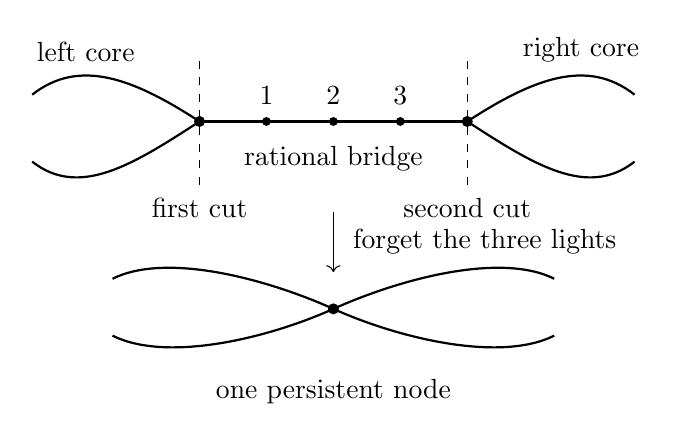
\begin{tikzpicture}[x=.85cm,y=.85cm]
  \draw[thick] (-4.5,.65) .. controls (-3.8,1.2) and (-3,.9) .. (-2,.25);
  \draw[thick] (-4.5,-.35) .. controls (-3.8,-.9) and (-3,-.4) .. (-2,.25);
  \draw[thick] (2,.25) .. controls (3,.9) and (3.8,1.2) .. (4.5,.65);
  \draw[thick] (2,.25) .. controls (3,-.4) and (3.8,-.9) .. (4.5,-.35);
  \draw[thick] (-2,.25) -- (2,.25);
  \fill (-2,.25) circle (2pt);
  \fill (2,.25) circle (2pt);
  \foreach \x/\lab in {-1/1,0/2,1/3}{
    \fill (\x,.25) circle (1.6pt);
    \node[above] at (\x,.36) {$\lab$};
  }
  \draw[dashed] (-2,-.7) -- (-2,1.2);
  \draw[dashed] (2,-.7) -- (2,1.2);
  \node[above] at (-3.7,1.0) {left core};
  \node[above] at (3.7,1.0) {right core};
  \node[below] at (0,.02) {rational bridge};
  \node[below] at (-2,-.75) {first cut};
  \node[below] at (2,-.75) {second cut};
  \draw[->] (0,-1.1) -- (0,-2.0);
  \node[right] at (.15,-1.55) {forget the three lights};
  \draw[thick] (-3.3,-2.1) .. controls (-2.5,-1.7) and (-1,-2.1) .. (0,-2.55);
  \draw[thick] (-3.3,-2.95) .. controls (-2.5,-3.35) and (-1,-3) .. (0,-2.55);
  \draw[thick] (0,-2.55) .. controls (1,-2.1) and (2.5,-1.7) .. (3.3,-2.1);
  \draw[thick] (0,-2.55) .. controls (1,-3) and (2.5,-3.35) .. (3.3,-2.95);
  \fill (0,-2.55) circle (2pt);
  \node[below] at (0,-3.45) {one persistent node};
\end{tikzpicture}
\caption{The two bounding nodes of a light-supported bridge.
After forgetting the lights the bridge contracts.  On a cut chart the
two node conditions contribute two normal cotangent factors.  The same
calculation applies when the two core branches belong to one component.
On the full exceptional surface, coincidence and the bridge class
have integrals $1$ and $2$, respectively, giving
$1-\tfrac12\cdot2=0$.}
\label{fig:bridge-cuts}
\end{figure}



\begin{lemma}\label{lem:weighted-pullback}
Let $g\geq2$, let the heavy set be empty, and pull the three-light
operations to any larger number of light labels by forgetting.
Under weight reduction from ordinary stable pointed curves,
$[i=j]$ pulls back to $\bar D_{ij}$ and $\beta_{g,\varnothing}$
pulls back to the normalized two-edge bridge sum used to define
$\beta_J^{\mathrm{st}}$.
Consequently the coefficient of the prescribed color word in the
signed product of all $F^0_{g,\varnothing}$ pulls back to $q(Y)$,
up to a nonzero rational scalar.
\end{lemma}

\begin{proof}
In codimension one, the inverse image of coincidence consists of
exactly the rational tails containing both labels.  At the generic
point of each tail, the difference of the two coarse positions is a
node-smoothing parameter times a nonzero difference of coordinates on
the tail.  Every multiplicity is therefore one.

Consider next the two bounding nodes of a weighted bridge.  Weight
reduction retaining all labels contracts light-only tails, not a bridge
with positive light mass.  Thus both bounding nodes exist already in
the source, and all the light labels assigned to the bridge originate
between those cuts.  The inverse image is supported on the
corresponding ordinary strata of codimension at least two.  At the
generic two-edge stratum the three labels are distinct on the bridge
and no component is contracted, so the pullback multiplicity is one.
Further collisions add edges and have higher codimension.  Normalized
graph sums count these local cut choices once, including for a loop.
This proves the supported codimension-two pullback assertion.

Forgetting commutes with reduction.  Finally, extracting a fixed color
word from signed averaging retains exactly the permutations preserving
that word, with their signs.  Depending on the averaging convention
there is a positive factorial denominator, but no zero scalar.
\end{proof}

\subsection{The local three-position calculation}

Over $\mathcal S_\Gamma$ let $C_v$ denote the smooth core curve at
vertex $v$.  For a fixed assignment of three labels, there is a coarse
position map
\begin{equation}\label{eq:coarse-positions}
 c:X^\Gamma(3)|_{\mathcal S_\Gamma}
       \longrightarrow
       C_{a(1)}\times_{\mathcal S_\Gamma}
       C_{a(2)}\times_{\mathcal S_\Gamma} C_{a(3)}.
\end{equation}
All products in this subsection are over the indicated heavy base.

\begin{lemma}\label{lem:three-position-blowup}
The map \eqref{eq:coarse-positions} is the iterated blowup obtained,
at each flag $p$, by first blowing up the locus where all three
assigned positions equal $p$, when present, and then the strict
transforms of the loci where two assigned positions equal $p$.
The latter centers are disjoint after the first blowup.
\end{lemma}

\begin{proof}
Extra components above a smooth pointed core are chains attached at
its flags.  A branch with no heavy endpoint and only light markings
would have a terminal light-only tail and is impossible.  Every level
of a chain carries positive light mass.

Choose a local parameter at a flag and write $x_i$ for the corresponding
coarse coordinate of label $i$.  The zero divisor of $x_i$ on the
configuration space is the sum, with multiplicity one, of the cuts
moving that label onto the expanded chain.  The multiplicity follows
from a one-node smoothing $xy=t$.  At a fixed point of the
configuration space these cuts form an initial segment of the
ordered chain.  Hence the products of smoothing parameters occurring
in the different $x_i$ are ordered by divisibility.  In particular,
each relevant pair or triple ideal is principal after pullback.
This gives a morphism to the first blowup and then to the successive
pair blowups; after the first step the pulled pair ideal is its strict
transform ideal times the exceptional line.

The blowup ratios recover the expanded configuration.  On a level
put its outward endpoint at infinity and its inward endpoint at zero.
The leading ratios of coarse coordinate differences are the ratios
of the light coordinates on that level, modulo common scaling.
Labels on separate levels give the limiting ratios zero or infinity.
Forgetting to pairs gives all these ratios compatibly, so the ratios
determine the levels and their configurations.  Automorphisms fixing
the core and the marked lights are trivial.  The resulting
representable map to the iterated blowup is therefore quasi-finite.
It is also proper and birational.  The target is smooth, and the
source is smooth by weighted deformation theory; working on
an etale chart of the core data, a proper birational quasi-finite map
to this normal target is an isomorphism
\cite[Tags~02LS and~0AB1]{Stacks}.

In the first exceptional plane, the strict pair centers meet at the
three distinct coordinate points, proving their disjointness.
The constructions at distinct flags have disjoint centers.
\end{proof}

Denote the total first exceptional divisor at a triple flag locus by
$E_{p,123}$.  Denote pair exceptional divisors, preferably pulled back
from the corresponding two-light spaces, by $E_{p,ij}$.
The blowup formula for Chow groups \cite[Proposition~6.7(e)]{Fulton} shows that a
codimension-two class on \eqref{eq:coarse-positions} has, in addition to
its main pullback, terms of the following forms:
\begin{equation}\label{eq:blowup-components}
 E_{p,ij}\,A_{p,ij},\qquad
 E_{p,123}\,D_p,\qquad
 a_p E_{p,123}^{\,2}.
\end{equation}
Here $A_{p,ij}$ is a divisor class on the remaining curve over the
base, $D_p$ is a base divisor class, and $a_p$ is a scalar on each
connected component of the base.  For clarity, if \(E_{p,ij}^{\mathrm{str}}\) is the strict pair
exceptional divisor and \(E_{p,ij}^{\mathrm{pull}}\) is pulled back
from two labels, then
\[
 E_{p,ij}^{\mathrm{pull}}
   =E_{p,ij}^{\mathrm{str}}+E_{p,123}.
\]
Multiplying the difference by a divisor on the remaining curve
restricts that divisor, on \(E_{p,123}\), to the flag section.
It is therefore a pulled base divisor. Replacing the strict version
by the pulled version changes only the
triple-exceptional-times-base-divisor term, and introduces no new
scalar multiple of \(E_{p,123}^2\).  Formula
\eqref{eq:blowup-components} includes assignments to different
vertices, in which some of the centers are simply absent.

When a raw class $F^0$ is pulled from an ancestor chart, its main
component is the small diagonal if all three labels are assigned to
one relevant descendant vertex, and is zero otherwise.  Away from
flags this is immediate.  The coincidence, bridge, and heavy-tail
corrections not seen there project to loci where all three coarse
positions are flags, of codimension three; they cannot alter a main
codimension-two class.

For the same pulled raw class, the divisor coefficients $A_{p,ij}$ in
\eqref{eq:blowup-components} are supported on flag sections of the
remaining curve, up to base divisor terms.  To see this, remove all
flags from that remaining curve.  Neither the raw class nor its main
diagonal pullback meets the pair exceptional locus over this open.
Intersecting with the exceptional divisor and pushing to its center
recovers its coefficient, with the usual negative self-intersection
sign for a codimension-two blowup center.  The coefficient is
therefore zero on this open.  Chow localization on the curve over the
base gives the assertion.

\begin{lemma}\label{lem:triple-exceptional-cancellation}
For the pullback of a raw cubic class $F^0$ from an ancestor chart, the
coefficient $a_p$ in \eqref{eq:blowup-components} is zero at every
triple flag locus.
\end{lemma}

\begin{proof}
Work first over a field point of the smooth heavy base.  The full
fiber over three positions at one flag is the weighted chain space
with two heavy endpoints and three lights, the Losev--Manin surface
\cite[Theorems~2.2 and~2.6.3]{LosevManin},
\cite[\S6.4]{Hassett}. By
Lemma~\ref{lem:three-position-blowup}, it is the first exceptional
$\mathbb P^2$ blown up at its three pair-collision points.
The total class $E_{p,123}$ restricts to the pullback of
$\mathcal O_{\mathbb P^2}(-1)$; hence
\begin{equation}\label{eq:exceptional-square}
 \int E_{p,123}^{\,2}=1.
\end{equation}
Main pullbacks, pair terms multiplied by a remaining-position divisor,
and base terms have integral zero on this fiber.  Thus this integral
detects exactly $a_p$.

The coincidence term gives one: its locus is the single transverse
configuration in which the three lights coincide away from the
endpoints.  We distinguish new and inherited flags relative to the
ancestor supplying the raw cubic.  Suppose first that $p$ is a new cut
flag.  There is one pair of bounding nodes isolating the chain carrying
the three lights.
This remains true on the boundary of the chain space.  Indeed, a
subcurve contracted upon forgetting the lights has two endpoint flags
and no persistent heavy marking; every component has at least two
incident branches before counting lights, so the component tree must
be a chain, with positive light mass on every level.  Its extreme
bounding nodes are uniquely determined.

With these cuts distinguished, as in Figure~\ref{fig:bridge-cuts},
the bridge locus is a regular
two-node condition in a versal deformation chart.  Its two normal
lines are the tensor products of the corresponding branch tangent
lines.  The core factors are constant on our fiber, so its
self-intersection restricts to
\begin{equation}\label{eq:bridge-normal}
 (-\psi_0)(-\psi_\infty)=\psi_0\psi_\infty.
\end{equation}
The normalized bridge sum counts this local branch once.  This
argument also treats a self-node: one distinguishes the two branches
before applying the normal formula, and the graph automorphism factor
removes the duplicate ordering.

Reduction from $\Mbar_{0,5}$ to the chain space preserves both heavy
cotangent lines.  A rational component carrying a heavy mark cannot
be contracted when the other three weights are decreased but remain
positive.  The genus-zero string recurrence gives
\begin{equation}\label{eq:chain-cotangent-integral}
 \int_{\Mbar_{0,5}}\psi_0\psi_\infty
   =\int_{\Mbar_{0,4}}\psi_0
     +\int_{\Mbar_{0,4}}\psi_\infty
   =2.
\end{equation}
The last equality follows by forgetting once more to
$\Mbar_{0,3}$.  Equivalently,
\eqref{eq:chain-cotangent-integral} is the degree-two case of the
genus-zero cotangent integral formula.  The bridge contribution to
$F^0$ is therefore $-\tfrac12\cdot2=-1$, canceling coincidence.

If instead $p$ is an inherited heavy flag, the relevant term is the
unique outer tail with that heavy marking and all three lights.
Its normal factor is $-\psi_0$ on the chain and the inserted
$\psi_p$ is $\psi_\infty$.  Thus
$\delta_{p,123}\psi_p$ has integral $-2$, and its coefficient
$+\tfrac12$ again cancels coincidence.  No other bridge or heavy-tail
type meets this fiber: after the lights are forgotten its contracted
locus is this specified node or this specified heavy mark.

We have shown that the scalar coefficient in
\eqref{eq:blowup-components} is zero on every connected smooth-core
base component.  This proves the result over that base.
\end{proof}

\subsection{Controlled pure lifts}

For a smooth heavy core $\pi:C\to S$, choose a degree-one rational
class
\[
 e_C=
 \begin{cases}
 [p],&\text{if a heavy flag $p$ has been chosen},\\
 c_1(\omega_{C/S})/(2h-2),&\text{if $B=\varnothing$}.
 \end{cases}
\]
The second case occurs only for $h\geq2$.  As in the curve tensor
construction, put
\begin{equation}\label{eq:compact-centering}
 e_C'=e_C-\frac12\pi^*\pi_*(e_C^2),
 \qquad
 \eta_C=[\Delta_C]-e'_{C,1}-e'_{C,2}.
\end{equation}
Write $\Delta_C^{\mathrm{pure}}$ for the small diagonal projected by
$\eta_C$ in each of its three slots.  Expanding the three projectors
shows that
\begin{equation}\label{eq:nonpure-pair-singleton}
 \begin{gathered}
 [\Delta_{123}]-\Delta_C^{\mathrm{pure}}
 \quad\text{is a sum of pair--singleton products},\\
 \text{with singleton factors }1_C\text{ or }e_C'.
 \end{gathered}
\end{equation}
No numerical equivalence is used in this expansion: it is the
decomposition of the diagonal correspondence into the pure projector
and the two hyperbolic projectors.

\begin{proposition}[Controlled pure lifts]
\label{prop:controlled-lifts}
For every stable heavy type $(h,B)$ one can choose a symmetric class
$G_{h,B}\in\CH^2(X_{h,B}(3))$ with the following properties.
\begin{enumerate}[label=\textup{(\roman*)}]
\item
Over the smooth heavy base, $G_{h,B}$ is exactly the pullback of
$\Delta_C^{\mathrm{pure}}$ by the coarse-position map.
\item
Pull a raw cubic $F^0$, or one of these chosen pure lifts $G$, from any
ancestor chart to a compact descendant cut chart.  Its operation is
a sum of the chosen pure lifts at the relevant descendant vertices,
with all three labels assigned to that vertex, together with
pair-times-singleton operations and a residual cubic operation.
\item
The singleton operations in \textup{(ii)}, and all their further
pullbacks through cuts and light forgetting, are controlled as
follows.  Over fixed smooth core data their restrictions lie
componentwise in the span of the unit, the canonical class, and the
flag points.  On any smooth test family the same statement holds
modulo classes supported over positive base codimension.
\item
On the current smooth-core open the residual operation in
\textup{(ii)} is a finite sum of classes containing a pulled base
divisor factor.  The base divisor may come from the current heavy
base or from a compact ancestor base.  Consequently its pullback to
every smooth test family is zero operationally after removing a
positive-codimension subset of that test base.
\end{enumerate}
All expansions preserve the color multiset.  They may always use one
and the same chosen $G$ and centering at a given current vertex,
regardless of which ancestor supplied the operation.
\end{proposition}

\begin{proof}
First work on the smooth heavy base of the class itself.  The blowup
decomposition \eqref{eq:blowup-components} and
Lemma~\ref{lem:triple-exceptional-cancellation} express $F^0$ as the
pullback of the small diagonal, plus pair-exceptional-times-singleton
terms and triple-exceptional-times-base-divisor terms.  Subtract these
terms, and also subtract \eqref{eq:nonpure-pair-singleton}.

These subtractions have compact extensions with the required
structure.  A pair exceptional divisor extends as the heavy-flag
tail boundary on the two-light space; a triple exceptional divisor
extends as its three-light counterpart.  Divisor coefficients on
the heavy base extend by Chow localization.  Pair coefficients may
also be extended by Chow localization on the smooth compact
two-light stack.  The singleton factors have specific extensions:
use units, the heavy sections, the relative dualizing line on the
one-light universal curve, and base classes.  In particular we do
not choose an arbitrary compact extension of the pure diagonal.
Define $G$ by making these structured subtractions from $F^0$, and
average over the three labels.  This gives \textup{(i)}.

Now pull to a deeper cut chart.  The raw $F^0$ has the decomposition
just proved there.  Its main component is the sum of the small
diagonals of the relevant descendant vertices.  Replace each by the
corresponding chosen $G$ plus its structured corrections.
Inherited pair-times-singleton subtractions retain that form:
forgetting commutes with cutting, so the pair coefficient remains a
two-label operation and the singleton remains a one-label operation.
The former is allowed to be arbitrary.  For the latter, the
normalization formula for the dualizing line gives the canonical
class plus the new branch points on each component.  A section
either lies on the relevant component or has zero restriction there;
base terms remain base terms.  This proves the asserted span and its
stability under further cuts.

The only other corrections are exceptional divisors multiplied by
base divisor classes.  On pulling an inherited correction, the
exceptional factor need not have a special form, but its base
divisor factor remains pulled from the ancestor heavy base.
The same description applies to the new corrections on the current
chart.  Thus the residual over its smooth-core open is of the form
\begin{equation}\label{eq:controlled-residual}
 \sum_j H_j\cdot\rho_j^*D_j,
\end{equation}
where $H_j$ is a one-codimensional three-label operation and $D_j$
is a divisor class on a current or ancestor heavy base, with the
natural induced map $\rho_j$.
Extending this decomposition to the compact chart can also leave a
difference supported over its heavy boundary, by Chow localization.
Include that difference in the residual operation.  Its restriction to
the smooth-core open is zero, so the residual there still has precisely
the form \eqref{eq:controlled-residual}.

To verify the last assertion after an arbitrary smooth test base
change $S$, represent each pulled rational divisor class by the
first Chern class of a rational line bundle.  A rational
trivialization makes it zero off a divisor of $S$.  After removing
the finite union of these divisors, every summand of
\eqref{eq:controlled-residual} is zero as an operational class.
This remains true if the image of $S$ lies inside a divisor on an
ancestor base: it is the pulled line bundle on $S$, not a presumed
transverse pullback of its original supporting cycle, that is used.
The base corrections in $e_C'$ are covered by the same argument.

Finally, if a previous operation used a different centering or a
different inherited presentation, expand it through its raw $F^0$
and the structured subtractions defining that presentation.  The
preceding argument again leaves the same allowed pair and singleton
terms, and a residual of the stated form on the smooth-core open.
We may therefore re-expand to
the fixed choice of $G$ at every current vertex.  Assignment
conditions can be imposed separately on the pair and singleton
factors by making their operations zero on the other components of
the disjoint union \eqref{eq:cut-chart}.  All steps occur before
inserting colors, and so preserve their multiset.
\end{proof}

\begin{remark}\label{rem:family-not-fiber}
The conclusion in Proposition~\ref{prop:controlled-lifts}\textup{(iv)}
is stronger than vanishing on individual geometric fibers.  It gives
operational vanishing on an open of every smooth test family,
including families mapping into a special locus of the heavy base.
This is the form needed when the remaining operation is multiplied
by an arbitrary cycle and Chow localization is used to lower its
base support.  Likewise, on the smooth-core open the equality in
\textup{(i)} is an equality of relative Chow correspondences.
Smooth proper base change for their pull, intersection, and push
operations identifies it with the centered tensor construction on
any such test family.
\end{remark}

\section{Support induction and Chow vanishing}
\label{sec:support}

We now combine the arbitrary-color bound of
Lemma~\ref{lem:large-vertex-test} with the compact lifts of
Proposition~\ref{prop:controlled-lifts}.  We will make successive parts
of the complete product of three-color entries vanish over dense opens
of its base support, until no support remains.  Throughout this section,
\[
 g=10^{60},\qquad D_*=\binom g3,\qquad n=3D_*,
 \qquad U_0=\Q^g.
\]
The basis of \(U_0\) is the set of colors.  An \emph{entry} is one factor
with three specified color inputs.  Initially there is one entry for each
increasing triple of distinct basis colors.  Products and their
factorizations are taken in the sign-coinvariant operation algebra of the
weighted spaces from the preceding section.

The graph charts, their compact heavy bases, and their smooth-core opens
will be denoted by
\[
 X^\Gamma(k),\qquad \mathcal B_\Gamma,\qquad
 \mathcal S_\Gamma\subset\mathcal B_\Gamma,
\]
respectively.  Every graph in this section has unmarked type \((g,0)\);
its vertex flags are heavy marks.  An operation supported on a vertex is
zero on assignment components on which its active labels are not all at
that vertex.

\subsection{Advancing support with an arbitrary multiplier}

Boundary-support methods also appear in tautological vanishing results
such as \cite[Theorem~1.1]{GraberVakil}, where support is measured by
rational components. Here we lower the dimension of the image in the
heavy base, using operational vanishing over smooth test families.
We first make this induction precise.  A term in it consists of
active operations, pulled to disjoint sets of light labels, acting on a
cycle on the full labeled chart.  The cycle need not factor over the
labels or over the vertices.

\begin{lemma}[Support advancement]
\label{lem:support-advancement}
Let a cycle multiplier on \(X^\Gamma(n)\) have base image contained in an
irreducible closed subspace \(Z\subset\mathcal B_\Gamma\).  After passing
to a refinement if necessary, suppose that its generic base image lies
in \(\mathcal S_\Gamma\).  Let \(L\) be a factor involving a specified
subset of the active entries.

Suppose that the pull of \(L\) vanishes operationally over a dense open
of a smooth test family dominating \(Z\cap\mathcal S_\Gamma\).  Then its
action can be written as a finite sum of cycles with strictly smaller
base-image dimension.  Only the entries in \(L\) are consumed.

More precisely, take a smooth test base \(S\), proper and generically
finite over \(Z\cap\mathcal S_\Gamma\).  If the vanishing holds off base
codimension at least \(a\), the terms remaining over \(\mathcal S_\Gamma\)
have base-image dimension at most \(\dim Z-a\).  The other terms lie over
\(Z\setminus\mathcal S_\Gamma\) and require a strict graph refinement.
If one first replaces \(S\) by the total space of one of its curve
families to obtain a section, the corresponding bound is
\(\dim Z-a+1\).
\end{lemma}

\begin{proof}
The proper cut-chart maps cover the preimages of boundary strata.
Consequently a cycle whose generic heavy curve has a finer dual graph
can be lifted to a chart of that graph.  These lifts do not increase the
dimension of its base image: heavy gluing is finite.

We use the following elementary property of rational Chow groups.  If
\(T'\to T\) is proper and surjective, every integral cycle on \(T\) has,
after multiplication by a nonzero rational number, a proper lift
generically finite over it.  Indeed, choose a closed point of the fiber
over its generic point, take its finite residue-field extension, and
close up that point.  The pushforward is the original cycle multiplied
by the generic degree.  The same property holds for the finite-type Deligne--Mumford charts
here with rational coefficients \cite[Proposition~B.19]{BaeSchmitt}.

For the test base, take a finite level cover of the smooth heavy-curve
stacks and resolve the appropriate component over
\(Z\cap\mathcal S_\Gamma\)
\cite[Theorems~1.0.2 and~1.0.3]{Wlodarczyk}.  This gives a smooth quasi-projective scheme
proper and generically finite over that space.  A full level of order at least three removes automorphisms in positive
genus \cite[Sections~5.3--5.4 and~5.14]{DeligneMumford},
\cite[IV.2.7--2.9 and IV.3.1--3.2]{DeligneRapoport}; the genus-one
vertices here have flags, and smooth genus-zero factors are already
schemes.  Lift the cycle multiplier properly to the resulting family by
the preceding argument.

Let \(A\subset S\) have codimension at least \(a\), and suppose that \(L\)
is zero operationally over \(S\setminus A\).  Its action on the lifted
multiplier restricts to zero there.  Chow localization expresses the
result as a pushforward of cycles lying over \(A\).  Projection formula
and proper pushforward return this equality to the original family.
Because \(\dim S=\dim Z\), these cycles have base-image dimension at most
\(\dim Z-a\).  Closing up inside the inverse image of \(Z\) can introduce
additional cycles only over \(Z\setminus\mathcal S_\Gamma\), a proper
closed subset of \(Z\).  Refining their generic dual graphs places them
on the required cut charts.

To obtain a section of a smooth curve family \(C\to S\), pull that
family back along \(C\to S\), where it has its diagonal section.
The new test base is smooth and has dimension \(\dim Z+1\).
Although this base change is not generically finite, the cycle multiplier
still admits a proper lift generically finite over itself: apply the
same generic-point argument to its pullback.  A support of codimension
at least \(a\) in the new base has image dimension at most
\(\dim Z+1-a\), proving the last assertion.

These operations concern the chosen factor \(L\).  All remaining
operations are carried along by pullback and projection formula and can
be applied afterwards to the resulting cycle multipliers.
\end{proof}

The operational hypothesis in this lemma is essential.  In its
applications below, it follows from identities over smooth test
families, rather than from identities separately on geometric fibers.
For a pure operation, Proposition~\ref{prop:controlled-lifts} identifies
its restriction with a pullback from a smooth curve power.  Vanishing
of its Chow class on that power is therefore operational vanishing and
can be pulled further to any cycle multiplier.  The formation of the
projector and the projected diagonal commutes with these base changes:
the relative diagonals and the integrations along smooth proper curve
powers have the requisite flat or refined-Gysin base-change identities.
For residual operations, the explicit base-divisor factors in
Proposition~\ref{prop:controlled-lifts} give the required open vanishing.
The same is true of the controlled singleton relations below.

There is also no restriction on the multiplier hidden in our use of
sign coinvariants.  In characteristic zero, signed averaging identifies
coinvariants with the corresponding signed invariant subspace.  A
factorization \(L*H\) of operations becomes a sum over shuffles of
products of the separately averaged \(L\) and \(H\), pulled to disjoint
slot sets.  In each summand, apply \(L\) first to the multiplier.
The factor \(H\) remains an averaged operation on its own active slots;
it is pulled equivariantly through later cuts before it acts.
This proves that the lemma applies repeatedly, even after the multiplier
has become an arbitrary cycle produced by an earlier step.
More explicitly, every later factorization of \(H\) is first an equality
of its signed-average representatives on its own active slots.  Pull
that equality to the full chart and only then cap with the multiplier.
No permutation is applied to the multiplier, and no invariance of the
multiplier is required.  Restriction to an assignment component or
pullback through a further cut preserves this equality.

Initially the heavy base has dimension \(3g-3\).  Every advancement
strictly lowers the base-image dimension.  Thus on any branch of the
finite expansions there can be at most
\begin{equation}
\label{eq:advancement-number}
 3g-2
\end{equation}
advancements before the support is empty.

\subsection{The elementary vanishing tests}

On a current chart, Proposition~\ref{prop:controlled-lifts} expands an
ancestor entry into pure entries at current vertices, products of a pair
operation with a controlled singleton, and residual cubic operations.
Call the pair-times-singleton terms \emph{noise entries}.
Perform these expansions one entry at a time.  If a residual summand is
chosen, apply Lemma~\ref{lem:support-advancement} to it immediately, at
the cost of that one entry.  We therefore never retain residual entries
while counting the pure and noise entries.

The pure entries at any one vertex always use the same chosen symmetric
class \(G_{h,B}\).  This is important both for the finite coefficient
bound and for the common-color test below.

\begin{lemma}[Noise and small-genus tests]
\label{lem:elementary-entry-tests}
Set
\[
 R_\Gamma=2|V(\Gamma)|+2|E(\Gamma)|.
\]
If \(R_\Gamma+1\) noise entries have their singleton at the same color,
their product advances support while consuming those entries.
If a genus-\(h\) vertex has more than \(\binom{2h}{3}\) pure entries,
the product of any \(\binom{2h}{3}+1\) of them advances support.
\end{lemma}

\begin{proof}
Over smooth generic core data, the one-light space at a vertex is its
curve.  The permitted singleton classes lie in the span of its unit,
canonical class, and flag points.  Over all vertices this gives a space
of dimension at most
\[
 \sum_v(2+|B_v|)=2|V|+2|E|=R_\Gamma.
\]
A one-slot operation is odd in the sign-coinvariant algebra.
At a fixed color, a product of \(R_\Gamma+1\) such elements is zero by
multilinearity and alternation.  The accompanying pair operations have
even arity and can be grouped separately.  This proves the first
vanishing, and it holds on an open of each smooth test family by the
controlled singleton descriptions and Chow localization.

For the second assertion apply Proposition~\ref{prop:tensor-test}.
Every tested pure entry is a value of the same odd-coefficient form
\(\varphi\in\mathfrak B\otimes\bigwedge^3 W_h^\vee\).
Its values belong to the span of at most \(\binom{2h}{3}\) odd
coefficients.  A longer product vanishes by supercommutativity.
The faithful same-map tensor test proves vanishing of the operation
modulo positive base support.  Only finitely many coefficient tests are
needed in a fixed arity, so their supports can be combined without
losing positive codimension.  Apply
Lemma~\ref{lem:support-advancement}.
\end{proof}

\subsection{A repeated-color test at a flagged vertex}

The surface test of Lemma~\ref{lem:large-vertex-test} is needed only
while one vertex has almost all the genus.  On every other chart a less expensive advancement follows
from the flag-centered curve algebra.

\begin{lemma}[Repeated-color advancement]
\label{lem:repeated-color}
Suppose that a vertex of genus \(h\) has a flag and that
\(k>\binom{h+1}{2}\) pure entries contain one common color \(i\).
Their product is a finite linear combination of products \(L*H\) with
the following properties:
\begin{enumerate}[label=\textup{(\roman*)}]
\item \(L\) involves at most \(h+2\) entries and vanishes modulo positive
base support;
\item \(H\) is still a product of individual pure entries at that vertex;
\item before removing the entries in \(L\), each term has the same color
multiset as the original product.
\end{enumerate}
Consequently each term admits a support advancement consuming at most
\(h+2\) entries.
\end{lemma}

\begin{proof}
A symmetric cubic class defines an alternating three-color operation.
Put the common color first in each entry.  The product, as a function of
the other \(2k\) inputs, factors through
\[
 \bigwedge^k\bigl(\bigwedge^2 U_0\bigr).
\]
This holds already on the compact chart: alternation inside a pair comes
from cubic symmetry, and interchange of two cubic entries has sign
minus because their arity is odd.

Let \(p\in\Q[\mathfrak S_{2k}]\) be the corresponding projector on the
input slots.  The exterior functor displayed above is zero on a vector
space of dimension \(h+1\).  By the Schur--Weyl decomposition and its row cutoff
\cite[Theorems~5.12.2, 5.18.4, and~5.22.1]{EtingofEtAl2011},
\(p\) lies in
the two-sided ideal generated by the alternator on \(h+2\) slots:
the quotient of the group algebra by that ideal acts faithfully on
tensor powers in dimension \(h+1\).  Indeed, its simple blocks are
indexed by partitions; precisely those with at most \(h+1\) rows
survive in that tensor power, and the \((h+2)\)-alternator generates
all the other blocks.  Thus \(p\) is a finite sum of
operators of the form
\[
 c\,\sigma\,\operatorname{Alt}_{h+2}\,\tau,
 \qquad c\in\Q,\quad \sigma,\tau\in\mathfrak S_{2k}.
\]
In one such term, first permute the color inputs by \(\tau\), and
interpret \(\sigma\) as their assignment to the pairs of entries.
Only entries meeting the \(h+2\) alternated positions vary during the
alternation.  There are at most \(h+2\) of them.  Group their alternated
product into \(L\), leaving the other entries in \(H\).
This proves the asserted factorization and the color-multiset statement.

It remains to prove the vanishing of \(L\).  Work on a smooth test base
modulo positive base support and center the curve projector at the chosen
flag section.  By Lemma~\ref{lem:point-centered-algebra}, its class \(e\)
has
\[
 \int e=1,\qquad \int e^2=0.
\]
Evaluation at the section is pairing with \(e\), is multiplicative, and
kills the pure odd space \(W_h\).  Hence for standard odd vectors \(u,v\),
their product in the coefficient Frobenius algebra has the form
\begin{equation}
\label{eq:point-centered-pair}
 uv=\omega(u,v)e+(uv)_{\mathrm{pure}}.
\end{equation}
There is no unit component, since its coefficient is the value of \(uv\)
at the section.

Test the colors by \(z:U_0\to W_h\), and write \(a=z(i)\).  Each entry
becomes
\[
 T_a(u,v)=\varphi(a,u,v),
\]
an alternating two-form with odd coefficients.  Contracting a variable
slot between two such entries gives zero.  To see this, the full
Frobenius contraction is, up to its fixed Koszul sign,
\[
 \int (au)(av)=0,
\]
because \(a\) is odd and \(a^2=0\).
The removed hyperbolic contraction in
\eqref{eq:point-centered-pair} is a multiple of \(\int e^2=0\);
orthogonality eliminates its mixed contractions.
The remaining symplectic contraction of the pure products is exactly
the stated contraction of the two cubic tensors.

An internal contraction of the two variable slots in a single \(T_a\)
is one and the same odd scalar, say \(\ell(a)\), up to the orientation
sign.  Two internal contractions in distinct entries therefore give
zero, because \(\ell(a)^2=0\).

After alternation, \(L\) is an ordinary alternating
\((h+2)\)-form on \(W_h\), with coefficients in the supercommutative
algebra.  Every summand of its double symplectic contraction is zero:
if one contraction joins distinct entries, perform that external
contraction first; otherwise the two contractions are internal in
distinct entries and give the square just considered.  All other
variables can be held arbitrary in the external identity, so this
reasoning also covers chains of contractions.

For \(h\ge2\), double contraction
\[
 \bigwedge^{h+2}W_h^\vee
 \longrightarrow \bigwedge^{h-2}W_h^\vee
\]
is injective by symplectic Lefschetz decomposition.  For \(h=0,1\),
the source alternation is already zero.  Thus every color test of \(L\)
vanishes.  Proposition~\ref{prop:tensor-test} and
Lemma~\ref{lem:support-advancement} finish the proof.
\end{proof}

\subsection{The finite color budget}

Set
\begin{equation}
\label{eq:color-constants}
 K=10^5,\qquad m_0=2000g^{2/3},\qquad
 C_K=\binom{2K}{3}.
\end{equation}
These are integers.  Reserve \(4K+20\) disjoint sets of \(m_0\) basis
colors each, and let \(S_0\) be all the remaining colors.  This is possible
because
\[
 \frac{(4K+20)m_0}{g}
   =8.0004\cdot10^{-12}<0.1;
 \qquad |S_0|>0.9g.
\]
For a current graph put
\[
 b=\max_v h_v,\qquad l=g-b.
\]
Under refinement the maximum vertex genus cannot increase, so \(l\)
cannot decrease.  The number of edges cannot decrease either.
Unmarked stability gives
\begin{equation}
\label{eq:global-noise-bound}
 |V|\le2g-2,\qquad |E|\le3g-3,\qquad R_\Gamma\le10g.
\end{equation}

An advancement by a residual entry, by a noise test, by a small-genus
test, or by Lemma~\ref{lem:repeated-color} will be called
\emph{ordinary}.  These are descriptions of the cost in entries, not
additional geometric assumptions.

The two regimes below use different information about the remaining
colors.  While \(l<K\), we remove whole entries without changing the
three colors of any retained entry; the reserved blocks can therefore
be counted by their original triples.  We use the repeated-color
rewrites only once \(l\ge K\).  They can change which colors occur
together in an entry, but preserve the total multiset of color
occurrences before the advancing factor is removed.  In that regime
we count occurrences in \(S_0\).  Since \(l\) cannot decrease, we never
need an original-triple count after making such a rewrite.

\paragraph{Small genus deficit: \(l<K\).}
There is a unique vertex of genus \(b\), since \(b>g-K>g/2\).
The total genus of all the others is at most \(l\), and stability gives
\begin{equation}
\label{eq:small-graph-size}
 |V|-1\le2l,\qquad |E|\le3l,\qquad R_\Gamma\le10K+2.
\end{equation}
For completeness, sum \(2h_v-2+\operatorname{val}(v)\ge1\) over all
vertices except the large one.  The sum equals
\(2l-\operatorname{val}(v_{\mathrm{large}})\), proving the first
inequality.  The genus formula then gives the second.

After expanding the active entries, use a residual immediately.
If a color occurs as a singleton in more than \(R_\Gamma\) noise entries,
use Lemma~\ref{lem:elementary-entry-tests}.  Otherwise there are at most
\(g(10K+2)\) noise entries.  If a small vertex has more than \(C_K\)
pure entries, use the same lemma there.  Otherwise the number of pure
entries off the large vertex is at most \(2K C_K\).
Each ordinary advancement in this regime costs at most
\[
 M_K=\max\{10K+3,C_K+1\}=C_K+1.
\]
As specified above, retained entries in this regime still have their
original triples, including those internal to each unused reserved
block.

Suppose none of these ordinary tests applies.  Choose a reserved color
block \(E_0\) that has not been used for a large-vertex test.  Let
\(D_0=\binom{m_0}{3}\).  Among its original \(D_0\) entirely internal
entries, the number that are no longer active pure entries at the large
vertex is at most
\begin{equation}
\label{eq:small-loss}
 3gM_K+g(10K+2)+2K C_K
 <10^{17}g<0.01D_0.
\end{equation}
Here \eqref{eq:advancement-number} bounds all preceding ordinary losses.
Earlier large-vertex tests used only entries internal to different,
disjoint reserved blocks, so they removed none of these entries.
The numerical inequalities follow from
\[
 C_K<1.334\cdot10^{15},
 \qquad D_0>10^9g^2,
 \qquad g=10^{60}.
\]
Thus more than \(0.99D_0\) internal entries remain pure at the large
vertex.

Consume the product of all those entries.  On a smooth test base,
obtain a section if necessary as in
Lemma~\ref{lem:support-advancement}.  Its dimension is at most \(3g-2\);
since \(b>g-K\),
\[
 3g-2<(b-1)^2-1.
\]
We may therefore use Lemma~\ref{lem:large-vertex-test}.
Choose an even integer \(e\) between \(m_0/2-2\) and \(m_0/2\).
For \(d_e=\binom e3\) and \(t_b=25(b-1)^2-1\), the explicit bounds are
\[
 d_e>D_0/10,\qquad t_b<25g^2,\qquad t_b<d_e/2,
\]
and consequently
\begin{equation}
\label{eq:large-test-threshold}
 D_0-d_e/2+t_b
   <(0.95+2.5\cdot10^{-8})D_0<0.99D_0.
\end{equation}
For the first bound, \(m_0\ge128\) and
\[
 \frac{\binom e3}{\binom{m_0}3}
 \ge \left(\frac12-\frac4{m_0}\right)^3>\frac1{10}.
\]
The selected product thus vanishes modulo base support of codimension
at least \(b-1\).  Applying
Lemma~\ref{lem:support-advancement}, it either lowers the base-image
dimension by at least \(b-2>g-K-2\), or gives a boundary remainder
requiring a strict refinement.  Call this an \emph{expensive}
advancement and mark \(E_0\) as used.

There are enough fresh blocks for every such advancement.
Those that require a refinement start with fewer than \(3K\) edges by
\eqref{eq:small-graph-size}; along a branch there are at most \(3K+1\)
of them.  Every other expensive advancement lowers the base-image
dimension by at least \(g-K-2\).  There can be at most three such
advancements with nonempty resulting support, because
\[
 4(g-K-2)>3g-3.
\]
A fourth can be terminal, making the support empty.
In total at most \(3K+5<4K+20\) blocks are needed.
No expensive advancement consumes an occurrence of a color in \(S_0\).

\paragraph{Large genus deficit: \(l\ge K\).}
Once this regime is reached it persists.  We continue to expand
ancestors using the same pure lift at each current vertex and peel
residuals immediately.  A noise test consumes at most \(10g+1\) entries.
If no such test applies, at most \(10g^2\) noise entries remain.

All ordinary advancements on the entire preceding path, including
those in the small-deficit regime, cost at most \(11g\) entries each:
\[
 C_K+1<11g,\qquad 10g+1<11g,\qquad h_v+2<11g.
\]
There have been at most \(3g-2\) advancements in total.
Each consumed entry has three color occurrences.  The cumulative
ordinary loss of occurrences in \(S_0\) is therefore less than
\(99g^2\).  The unpeeled noise accounts for at most another \(30g^2\).
Expensive advancements used no \(S_0\) colors.  Hence the number of
pure occurrences of colors from \(S_0\) is at least
\begin{equation}
\label{eq:remaining-pure-occurrences}
 |S_0|\binom{g-1}{2}-140g^2.
\end{equation}
The allowance \(140g^2\) is larger than the sum \(129g^2\) of the
two losses just obtained.
The permutations used in Lemma~\ref{lem:repeated-color} preserve the
color multiset before its advancing factor is removed, so the same
bound remains valid after any number of those rewrites.

Discard any identically zero product, in particular a product containing
a pure entry with a repeated color.  Suppose that every color
\(i\in S_0\), at every vertex \(v\), belongs to at most
\(\binom{h_v+1}{2}\) pure entries.  The total number of pure occurrences
would then be at most
\[
 |S_0|\sum_v\binom{h_v+1}{2}
 \le \frac{|S_0|}{2}(b+1)\sum_v h_v
 \le \frac{|S_0|g(b+1)}2.
\]
This contradicts \eqref{eq:remaining-pure-occurrences}.  Indeed, the
lower bound minus this upper bound is
\[
 \frac{|S_0|}{2}\bigl(g(l-4)+2\bigr)-140g^2
 >\bigl(0.45(K-4)-140\bigr)g^2>0.
\]
There is therefore a color and vertex to which
Lemma~\ref{lem:repeated-color} applies.
Every vertex in this regime has a flag: a connected graph without any
flags at one of its vertices could only be the one-vertex, no-edge
graph, for which \(l=0\).
The lemma supplies another ordinary advancement, at the claimed cost.

\subsection{Completion}

\begin{theorem}
\label{thm:chow-vanishing}
The class \(Y\in\Salg_{g,n}\) constructed above satisfies
\[
 q_{g,n}(Y)=0
 \quad\text{in }\CH^*(\Mbar_{g,n};\Q).
\]
\end{theorem}

\begin{proof}
Begin on \(X_{g,\varnothing}(n)\) with the product of the cubic
operations \(F^0_{g,\varnothing}\), one for each increasing color triple,
and with the fundamental cycle as multiplier.  Apply
Proposition~\ref{prop:controlled-lifts} and the preceding induction.
At every stage, each nonzero branch admits an advancement: use a
residual or noise test when available, the small-vertex and reserved-block
tests if \(l<K\), and otherwise the repeated-color test.
The counts show that all required active entries and unused blocks are
available at the moment they are needed.

Each individual expansion and localization involves finitely many
cycles.  Each branch has length at most \(3g-2\), by
\eqref{eq:advancement-number}.  Thus the process ends with empty
support and proves that the full product is zero in the sign-coinvariant
Chow group of the weighted space.

The weighted-to-unweighted comparison in
Lemma~\ref{lem:weighted-pullback} identifies the pullback of the
raw cubic with \(q(F_J^{\mathrm{st}})\).  After signed averaging, the
coefficient of the ordered color word \(\mathbf i\) is a nonzero
rational scalar times
\[
 q_{g,n}\!\left(
 \sum_{\tau:\,\tau\mathbf i=\mathbf i}
   \operatorname{sgn}(\tau)\,
   \tau\!\left(\prod_J F_J^{\mathrm{st}}\right)
 \right)=q_{g,n}(Y).
\]
Pulling back the zero weighted class proves the theorem.
\end{proof}

\begin{proof}[Proof of Theorem~\ref{thm:main}]
Theorem~\ref{thm:chow-vanishing} places \(Y\) in the Chow kernel.
Proposition~\ref{prop:detector} supplies a linear map annihilating the
specified Pixton span and taking a nonzero value on \(Y\).  Thus
\[
 Y\in\ker q_{g,n}\setminus\Pspan_{g,n}.
\]
The stable pair \(g=10^{60}\), \(n=3\binom g3\) is a counterexample to
the proposed equality for all stable pairs.
\end{proof}

\begin{thebibliography}{Stacks}

\bibitem[Abr]{Abrams1996}
L.~Abrams,
\emph{Two-dimensional topological quantum field theories and Frobenius algebras},
J. Knot Theory Ramifications \textbf{5} (1996), no.~5, 569--587.
\href{https://doi.org/10.1142/S0218216596000333}{doi:10.1142/S0218216596000333}.

\bibitem[AC]{ArbarelloCornalba1996}
E.~Arbarello and M.~Cornalba,
\emph{Combinatorial and algebro-geometric cohomology classes on the moduli spaces of curves},
J.\ Algebraic Geom.\ \textbf{5} (1996), no.~4, 705--749.
\href{https://arxiv.org/abs/alg-geom/9406008}{arXiv:alg-geom/9406008}.

\bibitem[ADO]{ADOJouanolou}
A.~Asok, A.~Dubouloz, and P.~A.~{\O}stv{\ae}r,
\emph{Geometric models for algebraic suspensions},
Int.\ Math.\ Res.\ Not.\ \textbf{2023} (2023), no.~20, 17788--17821.
\href{https://doi.org/10.1093/imrn/rnad094}{doi:10.1093/imrn/rnad094}.
\href{https://arxiv.org/abs/2112.08241v2}{arXiv:2112.08241v2}.

\bibitem[BSch]{BaeSchmitt}
Y.~Bae and J.~Schmitt, with an appendix jointly with J.~Skowera,
\emph{Chow rings of stacks of prestable curves I},
Forum Math. Sigma \textbf{10} (2022), e28.
\href{https://doi.org/10.1017/fms.2022.21}{doi:10.1017/fms.2022.21}.

\bibitem[Bea]{Beauville1983}
A.~Beauville,
\emph{Quelques remarques sur la transformation de Fourier dans l'anneau de Chow
d'une vari\'et\'e ab\'elienne},
in \emph{Algebraic Geometry (Tokyo/Kyoto, 1982)},
Lecture Notes in Math. \textbf{1016}, Springer, 1983, 238--260.
\href{https://doi.org/10.1007/BFb0099965}{doi:10.1007/BFb0099965}.

\bibitem[BF]{BF}
K.~Behrend and B.~Fantechi,
\emph{The intrinsic normal cone},
Invent.\ Math.\ \textbf{128} (1997), 45--88.
\href{https://doi.org/10.1007/s002220050136}{doi:10.1007/s002220050136}.
Preprint version:
\href{https://arxiv.org/abs/alg-geom/9601010v1}{arXiv:alg-geom/9601010v1}.

\bibitem[BS]{BorelSerre}
A.~Borel and J.-P.~Serre,
\emph{Le th\'eor\`eme de Riemann--Roch},
Bull.\ Soc.\ Math.\ France \textbf{86} (1958), 97--136.
\href{https://doi.org/10.24033/bsmf.1500}{doi:10.24033/bsmf.1500}.

\bibitem[BLR]{BLR}
S.~Bosch, W.~L\"utkebohmert, and M.~Raynaud,
\emph{N\'eron Models},
Ergebnisse der Mathematik und ihrer Grenzgebiete (3), vol.~21,
Springer-Verlag, Berlin, 1990.

\bibitem[Can]{Canning2025}
S.~Canning,
\emph{The tautological ring of $\overline{\mathcal M}_{g,n}$ is rarely Gorenstein},
Geom.\ Topol.\ \textbf{29} (2025), no.~7, 3905--3919.
\href{https://doi.org/10.2140/gt.2025.29.3905}{doi:10.2140/gt.2025.29.3905}.
Numbered statements refer to
\href{https://arxiv.org/abs/2406.10516v1}{arXiv:2406.10516v1}.

\bibitem[CLS]{CanningLarsonSchmitt2026}
S.~Canning, H.~Larson, and J.~Schmitt,
\emph{The Gorenstein property and Pixton's conjecture for compact type moduli},
\href{https://arxiv.org/abs/2607.02249v2}{arXiv:2607.02249v2}, 2026.

\bibitem[DM]{DeligneMumford}
P.~Deligne and D.~Mumford,
\emph{The irreducibility of the space of curves of given genus},
Publ.\ Math.\ IH\'ES \textbf{36} (1969), 75--109.
\href{https://www.numdam.org/item/PMIHES_1969__36__75_0.pdf}{Original article}.

\bibitem[DR]{DeligneRapoport}
P.~Deligne and M.~Rapoport,
\emph{Les sch\'emas de modules de courbes elliptiques},
in \emph{Modular Functions of One Variable II},
Lecture Notes in Mathematics \textbf{349}, Springer, 1973, 143--316.
\href{https://publications.ias.edu/sites/default/files/Number22.pdf}{Original article}.

\bibitem[EG]{EdidinGraham}
D.~Edidin and W.~Graham,
\emph{Equivariant intersection theory},
Invent.\ Math.\ \textbf{131} (1998), no.~3, 595--634.
Numbered statements refer to
\href{https://arxiv.org/abs/alg-geom/9609018v3}{arXiv:alg-geom/9609018v3}.

\bibitem[EGL]{EGL}
G.~Ellingsrud, L.~G\"ottsche, and M.~Lehn,
\emph{On the cobordism class of the Hilbert scheme of a surface},
J.\ Algebraic Geom.\ \textbf{10} (2001), no.~1, 81--100.
\href{https://arxiv.org/abs/math/9904095v1}{arXiv:math/9904095v1}.

\bibitem[EGH+]{EtingofEtAl2011}
P.~Etingof, O.~Golberg, S.~Hensel, T.~Liu, A.~Schwendner,
D.~Vaintrob, and E.~Yudovina,
\emph{Introduction to Representation Theory},
Student Mathematical Library \textbf{59}, American Mathematical Society, 2011.
\href{https://math.mit.edu/~etingof/representationtheorybook.pdf}{Author text}.

\bibitem[Fab]{Faber1999}
C.~Faber,
\emph{A conjectural description of the tautological ring of the moduli space of curves},
in \emph{Moduli of Curves and Abelian Varieties},
Aspects of Mathematics E33, Vieweg, Braunschweig, 1999, 109--129.
\href{https://arxiv.org/abs/math/9711218v1}{arXiv:math/9711218v1}.

\bibitem[Fog]{Fogarty}
J.~Fogarty,
\emph{Algebraic families on an algebraic surface},
Amer.\ J.\ Math.\ \textbf{90} (1968), no.~2, 511--521.
\href{https://doi.org/10.2307/2373541}{doi:10.2307/2373541}.

\bibitem[FM]{FultonMacPherson}
W.~Fulton and R.~MacPherson,
\emph{A compactification of configuration spaces},
Ann.\ of Math.\ (2) \textbf{139} (1994), no.~1, 183--225.
\href{https://doi.org/10.2307/2946631}{doi:10.2307/2946631}.

\bibitem[Ful]{Fulton}
W.~Fulton,
\emph{Intersection Theory},
second edition, Springer, 1998.
\href{https://doi.org/10.1007/978-1-4612-1700-8}{doi:10.1007/978-1-4612-1700-8}.

\bibitem[GP]{GP}
T.~Graber and R.~Pandharipande,
\emph{Localization of virtual classes},
Invent.\ Math.\ \textbf{135} (1999), 487--518.
\href{https://doi.org/10.1007/s002220050293}{doi:10.1007/s002220050293}.
Preprint version:
\href{https://arxiv.org/abs/alg-geom/9708001v2}{arXiv:alg-geom/9708001v2}.

\bibitem[GP03]{GraberPandharipande2003}
T.~Graber and R.~Pandharipande,
\emph{Constructions of nontautological classes on moduli spaces of curves},
Michigan Math.\ J.\ \textbf{51} (2003), no.~1, 93--109.
\href{https://arxiv.org/abs/math/0104057v2}{arXiv:math/0104057v2}.

\bibitem[GV]{GraberVakil}
T.~Graber and R.~Vakil,
\emph{Relative virtual localization and vanishing of tautological classes on moduli spaces of curves},
Duke Math.\ J.\ \textbf{130} (2005), no.~1, 1--37.
\href{https://arxiv.org/abs/math/0309227v3}{arXiv:math/0309227v3}.

\bibitem[GS]{GrossSchoen1995}
B.~H.~Gross and C.~Schoen,
\emph{The modified diagonal cycle on the triple product of a pointed curve},
Ann. Inst. Fourier \textbf{45} (1995), no.~3, 649--679.
\href{https://doi.org/10.5802/aif.1469}{doi:10.5802/aif.1469}.

\bibitem[Has]{Hassett}
B.~Hassett,
\emph{Moduli spaces of weighted pointed stable curves},
Adv.\ Math.\ \textbf{173} (2003), no.~2, 316--352.
\href{https://doi.org/10.1016/S0001-8708(02)00058-0}{doi:10.1016/S0001-8708(02)00058-0}.
Preprint version:
\href{https://arxiv.org/abs/math/0205009v1}{arXiv:math/0205009v1}.

\bibitem[Jan]{Janda}
F.~Janda,
\emph{Relations on $\overline{\mathcal M}_{g,n}$ via equivariant
Gromov--Witten theory of $\mathbb P^1$},
Algebraic Geometry \textbf{4} (2017), no.~3, 311--336.
\href{https://doi.org/10.14231/AG-2017-018}{doi:10.14231/AG-2017-018}.
Preprint version:
\href{https://arxiv.org/abs/1509.08421v3}{arXiv:1509.08421v3}.

\bibitem[JanD]{JandaDiscriminant}
F.~Janda,
\emph{Frobenius manifolds near the discriminant and relations in the tautological ring},
Lett.\ Math.\ Phys.\ \textbf{108} (2018), no.~7, 1649--1675.
\href{https://doi.org/10.1007/s11005-018-1047-2}{doi:10.1007/s11005-018-1047-2}.
Numbered statements refer to
\href{https://arxiv.org/abs/1505.03419v3}{arXiv:1505.03419v3}.

\bibitem[Keel]{Keel1992}
S.~Keel,
\emph{Intersection theory of moduli space of stable $n$-pointed curves of genus zero},
Trans.\ Amer.\ Math.\ Soc.\ \textbf{330} (1992), no.~2, 545--574.
\href{https://doi.org/10.1090/S0002-9947-1992-1034665-0}{doi:10.1090/S0002-9947-1992-1034665-0}.

\bibitem[Kle]{KleimanPicard}
S.~L.~Kleiman,
\emph{The Picard scheme},
\href{https://arxiv.org/abs/math/0504020v1}{arXiv:math/0504020v1}, 2005.

\bibitem[Kong]{Kong2026}
B.~Kong,
\emph{Tautological pushforwards of Hilbert schemes of points on curves and surfaces},
\href{https://arxiv.org/abs/2608.25447v1}{arXiv:2608.25447v1}, 2026.

\bibitem[Kre]{Kresch}
A.~Kresch,
\emph{Cycle groups for Artin stacks},
Invent.\ Math.\ \textbf{138} (1999), 495--536.
Numbered statements refer to
\href{https://arxiv.org/abs/math/9810166v1}{arXiv:math/9810166v1}.

\bibitem[Leh]{Lehn99}
M.~Lehn,
\emph{Chern classes of tautological sheaves on Hilbert schemes of points on surfaces},
Invent.\ Math.\ \textbf{136} (1999), 157--207.
\href{https://arxiv.org/abs/math/9803091v1}{arXiv:math/9803091v1}.

\bibitem[LZ]{LZ15}
G.~I.~Lehrer and R.~B.~Zhang,
\emph{The Brauer category and invariant theory},
J.\ Eur.\ Math.\ Soc.\ \textbf{17} (2015), 2311--2351.
\href{https://doi.org/10.4171/JEMS/558}{doi:10.4171/JEMS/558}.

\bibitem[LM]{LosevManin}
A.~Losev and Y.~Manin,
\emph{New moduli spaces of pointed curves and pencils of flat connections},
Michigan Math.\ J.\ \textbf{48} (2000), 443--472.
\href{https://doi.org/10.1307/mmj/1030132728}{doi:10.1307/mmj/1030132728}.
\href{https://arxiv.org/abs/math/0001003v2}{arXiv:math/0001003v2}.

\bibitem[Man]{Manolache}
C.~Manolache,
\emph{Virtual pull-backs},
\href{https://arxiv.org/abs/0805.2065v2}{arXiv:0805.2065v2}, 2011.

\bibitem[MOP1]{MOPSegre}
A.~Marian, D.~Oprea, and R.~Pandharipande,
\emph{Segre classes and Hilbert schemes of points},
Ann.\ Sci.\ \'Ecole Norm.\ Sup.\ (4) \textbf{50} (2017), no.~1, 239--267.
\href{https://doi.org/10.24033/asens.2320}{doi:10.24033/asens.2320}.
\href{https://arxiv.org/abs/1507.00688v2}{arXiv:1507.00688v2}.

\bibitem[MOP2]{MOPCombinatorics}
A.~Marian, D.~Oprea, and R.~Pandharipande,
\emph{The combinatorics of Lehn's conjecture},
J.\ Math.\ Soc.\ Japan \textbf{71} (2019), 299--308.
\href{https://arxiv.org/abs/1708.08129v2}{arXiv:1708.08129v2}.
Numbered statements refer to the December 2017 author manuscript,
\href{https://people.math.ethz.ch/~rahul/LehnF.pdf}{author version}.

\bibitem[Mil]{Milne2022}
J.~S.~Milne,
\emph{Algebraic Groups: The Theory of Group Schemes of Finite Type over a Field},
Cambridge Studies in Advanced Mathematics \textbf{170}, Cambridge University Press, 2017.
Numbered statements refer to the revised 2022 author version,
\href{https://www.jmilne.org/math/Books/iAG2022.pdf}{Algebraic Groups (2022)}.

\bibitem[Muk]{Mukai1981}
S.~Mukai,
\emph{Duality between $D(X)$ and $D(\widehat X)$ with its application to Picard sheaves},
Nagoya Math. J. \textbf{81} (1981), 153--175.
\href{https://doi.org/10.1017/S002776300001922X}{doi:10.1017/S002776300001922X}.

\bibitem[Mum]{Mumford1983}
D.~Mumford,
\emph{Towards an enumerative geometry of the moduli space of curves},
in \emph{Arithmetic and Geometry, Vol.~II}, Progress in Mathematics
\textbf{36}, Birkh\"auser, 1983, 271--328.
\href{https://doi.org/10.1007/978-1-4757-9286-7_12}{doi:10.1007/978-1-4757-9286-7\_12}.

\bibitem[Nit]{Nitsure}
N.~Nitsure,
\emph{Construction of Hilbert and Quot schemes},
\href{https://arxiv.org/abs/math/0504590v1}{arXiv:math/0504590v1}, 2005.

\bibitem[OP]{OPQuot}
D.~Oprea and R.~Pandharipande,
\emph{Quot schemes of curves and surfaces: virtual classes, integrals,
Euler characteristics},
Geom.\ Topol.\ \textbf{25} (2021), 3425--3505.
\href{https://doi.org/10.2140/gt.2021.25.3425}{doi:10.2140/gt.2021.25.3425}.
\href{https://arxiv.org/abs/1903.08787v2}{arXiv:1903.08787v2}.

\bibitem[OS]{OSullivan2011}
P.~O'Sullivan,
\emph{Algebraic cycles on an abelian variety},
J.\ Reine Angew.\ Math.\ \textbf{654} (2011), 1--81.
\href{https://doi.org/10.1515/crelle.2011.025}{doi:10.1515/crelle.2011.025}.
Numbered statements refer to
\href{https://arxiv.org/abs/0908.0626v1}{arXiv:0908.0626v1}.

\bibitem[PP]{PandharipandePixton2021}
R.~Pandharipande and A.~Pixton,
\emph{Relations in the tautological ring of the moduli space of curves},
Pure Appl.\ Math.\ Q.\ \textbf{17} (2021), no.~2, 717--771.
\href{https://doi.org/10.4310/PAMQ.2021.v17.n2.a7}{doi:10.4310/PAMQ.2021.v17.n2.a7}.
\href{https://arxiv.org/abs/1301.4561v2}{arXiv:1301.4561v2}.

\bibitem[PPZ]{PPZ}
R.~Pandharipande, A.~Pixton, and D.~Zvonkine,
\emph{Relations on $\overline{\mathcal M}_{g,n}$ via $3$-spin structures},
J.\ Amer.\ Math.\ Soc.\ \textbf{28} (2015), no.~1, 279--309.
Numbered statements and formulas refer to the corrected version
\href{https://arxiv.org/abs/1303.1043v3}{arXiv:1303.1043v3}.

\bibitem[PZ]{PZ2019}
R.~Pandharipande and D.~Zvonkine, with an appendix by D.~Petersen,
\emph{Cohomological field theories with non-tautological classes},
Ark. Mat. \textbf{57} (2019), no.~1, 191--213.
\href{https://doi.org/10.4310/ARKIV.2019.v57.n1.a10}{doi:10.4310/ARKIV.2019.v57.n1.a10}.

\bibitem[PetW]{PetersenWonderful}
D.~Petersen,
\emph{Poincar\'e duality of wonderful compactifications and tautological rings},
Int.\ Math.\ Res.\ Not.\ \textbf{2016} (2016), no.~17, 5187--5201.
Numbered statements refer to
\href{https://arxiv.org/abs/1501.04742v2}{arXiv:1501.04742v2}.

\bibitem[Pix]{Pixton}
A.~Pixton,
\emph{Conjectural relations in the tautological ring of
$\overline{\mathcal M}_{g,n}$},
\href{https://arxiv.org/abs/1207.1918v1}{arXiv:1207.1918v1}, 2012.

\bibitem[Pix26]{Pixton2026}
A.~Pixton,
\emph{The tautological ring of $\mathcal M_{25}$ is not Gorenstein},
\href{https://arxiv.org/abs/2609.15949v1}{arXiv:2609.15949v1}, 2026.

\bibitem[Rou]{Routis}
E.~Routis,
\emph{Weighted compactifications of configuration spaces and relative stable degenerations},
\href{https://arxiv.org/abs/1411.2955v1}{arXiv:1411.2955v1}, 2014.

\bibitem[RW]{RW15}
M.~Rubey and B.~W.~Westbury,
\emph{Combinatorics of symplectic invariant tensors},
Discrete Math.\ Theor.\ Comput.\ Sci.\ Proc., FPSAC 2015 (2015), 285--296.
\href{https://doi.org/10.46298/dmtcs.2508}{doi:10.46298/dmtcs.2508}.

\bibitem[STV]{STV}
T.~Sch\"urg, B.~To\"en, and G.~Vezzosi,
\emph{Derived algebraic geometry, determinants of perfect complexes,
and applications to obstruction theories for maps and complexes},
J.\ Reine Angew.\ Math.\ \textbf{702} (2015), 1--40.
\href{https://doi.org/10.1515/crelle-2013-0037}{doi:10.1515/crelle-2013-0037}.
Numbered statements follow the
\href{https://flore.unifi.it/retrieve/e398c37f-a432-179a-e053-3705fe0a4cff/crelle.pdf}{accepted-manuscript galley}.

\bibitem[Stacks]{Stacks}
The Stacks Project Authors,
\emph{The Stacks Project}, 2026.
\url{https://stacks.math.columbia.edu}.
Specific results are cited by their stable tags.

\bibitem[Tav]{TavakolRT}
M.~Tavakol,
\emph{The connection between $R^*(\mathcal C_g^n)$ and
$R^*(\mathcal M_{g,n}^{\mathrm{rt}})$},
J.\ Pure Appl.\ Algebra \textbf{222} (2018), no.~6, 1306--1315.
Preprint version, titled \emph{A conjectural connection between
$R^*(\mathcal C_g^n)$ and $R^*(\mathcal M_{g,n}^{\mathrm{rt}})$}:
\href{https://arxiv.org/abs/1412.5036v2}{arXiv:1412.5036v2}.

\bibitem[TV]{TV}
B.~To\"en and M.~Vaqui\'e,
\emph{Moduli of objects in dg-categories},
Ann.\ Sci.\ \'Ecole Norm.\ Sup.\ (4) \textbf{40} (2007), no.~3, 387--444.
\href{https://doi.org/10.1016/j.ansens.2007.05.001}{doi:10.1016/j.ansens.2007.05.001}.
Numbered statements follow the
\href{https://www.math.univ-toulouse.fr/~btoen/ttt.pdf}{April 2007 author manuscript}.

\bibitem[Wlo]{Wlodarczyk}
J.~W{\l}odarczyk,
\emph{Simple Hironaka resolution in characteristic zero},
\href{https://arxiv.org/abs/math/0401401v1}{arXiv:math/0401401v1}, 2004.

\end{thebibliography}

\end{document}
